\documentclass[12pt,letter]{article}\usepackage[]{graphicx}\usepackage[]{color}
%% maxwidth is the original width if it is less than linewidth
%% otherwise use linewidth (to make sure the graphics do not exceed the margin)
\makeatletter
\def\maxwidth{ %
  \ifdim\Gin@nat@width>\linewidth
    \linewidth
  \else
    \Gin@nat@width
  \fi
}
\makeatother

\definecolor{fgcolor}{rgb}{0.345, 0.345, 0.345}
\newcommand{\hlnum}[1]{\textcolor[rgb]{0.686,0.059,0.569}{#1}}%
\newcommand{\hlstr}[1]{\textcolor[rgb]{0.192,0.494,0.8}{#1}}%
\newcommand{\hlcom}[1]{\textcolor[rgb]{0.678,0.584,0.686}{\textit{#1}}}%
\newcommand{\hlopt}[1]{\textcolor[rgb]{0,0,0}{#1}}%
\newcommand{\hlstd}[1]{\textcolor[rgb]{0.345,0.345,0.345}{#1}}%
\newcommand{\hlkwa}[1]{\textcolor[rgb]{0.161,0.373,0.58}{\textbf{#1}}}%
\newcommand{\hlkwb}[1]{\textcolor[rgb]{0.69,0.353,0.396}{#1}}%
\newcommand{\hlkwc}[1]{\textcolor[rgb]{0.333,0.667,0.333}{#1}}%
\newcommand{\hlkwd}[1]{\textcolor[rgb]{0.737,0.353,0.396}{\textbf{#1}}}%
\let\hlipl\hlkwb

\usepackage{framed}
\makeatletter
\newenvironment{kframe}{%
 \def\at@end@of@kframe{}%
 \ifinner\ifhmode%
  \def\at@end@of@kframe{\end{minipage}}%
  \begin{minipage}{\columnwidth}%
 \fi\fi%
 \def\FrameCommand##1{\hskip\@totalleftmargin \hskip-\fboxsep
 \colorbox{shadecolor}{##1}\hskip-\fboxsep
     % There is no \\@totalrightmargin, so:
     \hskip-\linewidth \hskip-\@totalleftmargin \hskip\columnwidth}%
 \MakeFramed {\advance\hsize-\width
   \@totalleftmargin\z@ \linewidth\hsize
   \@setminipage}}%
 {\par\unskip\endMakeFramed%
 \at@end@of@kframe}
\makeatother

\definecolor{shadecolor}{rgb}{.97, .97, .97}
\definecolor{messagecolor}{rgb}{0, 0, 0}
\definecolor{warningcolor}{rgb}{1, 0, 1}
\definecolor{errorcolor}{rgb}{1, 0, 0}
\newenvironment{knitrout}{}{} % an empty environment to be redefined in TeX

\usepackage{alltt}

%########################################################################################
%            						PACKAGES
%########################################################################################

\usepackage{authblk} % for author affiliations
\usepackage{float} % for H in figures and tables
\usepackage{amsmath,amsthm,amssymb,bbm,mathrsfs,mathtools,xfrac} %math stuff

\usepackage[sort, numbers]{natbib}   % bibliography omit 'round' option if you prefer square brackets
\usepackage{placeins} % for \FloatBarrier
\usepackage[pagebackref=true,bookmarks]{hyperref}
\hypersetup{
	unicode=false,
	pdftoolbar=true,
	pdfmenubar=true,
	pdffitwindow=false,     % window fit to page when opened
	pdfstartview={FitH},    % fits the width of the page to the window
	pdftitle={Penalized LMM in Families},    % title
	pdfauthor={Sahir Rai Bhatnagar},     % author
	pdfsubject={Subject},   % subject of the document
	pdfcreator={Sahir Rai Bhatnagar},   % creator of the document
	pdfproducer={Sahir Rai Bhatnagar}, % producer of the document
	pdfkeywords={}, % list of keywords
	pdfnewwindow=true,      % links in new window
	colorlinks=true,       % false: boxed links; true: colored links
	linkcolor=red,          % color of internal links (change box color with linkbordercolor)
	citecolor=blue,        % color of links to bibliography
	filecolor=black,      % color of file links
	urlcolor=cyan           % color of external links
}
\usepackage[utf8]{inputenc} % for french accents
\usepackage[T1]{fontenc} % for french accents
\usepackage{ctable} % load after tikz. used for tables
\usepackage{array}
\newcolumntype{L}{>{\centering\arraybackslash}m{3cm}} % used for text wrapping in ctable
\usepackage{color, colortbl, xcolor, comment}
\usepackage{subfig}
\usepackage{tcolorbox} % for box around text
%\usepackage[ruled,vlined,linesnumbered,noresetcount]{algorithm2e}
\usepackage[ruled,vlined,noresetcount]{algorithm2e}
%\usepackage[american]{babel}
%\let\tnote\relax
\newtheorem{theorem}{Theorem}[section]
\newtheorem{proposition}{Proposition}[section]

%\usepackage{csquotes}



%\usepackage[style=apa,sortcites=true,sorting=nyt,backend=biber]{biblatex}
%\usepackage{epstopdf}

%\usepackage{tabulary}
%\usepackage{siunitx}
%\sisetup{output-exponent-marker=\ensuremath{\mathrm{e}}}
%\usepackage{setspace}
%\AtBeginEnvironment{tabulary}{\onehalfspacing}
%\usepackage{multirow}
%\usepackage{ctable} % NEED TO LOAD CTABLE AFTER TIKZ FOR SOME REASON
%\usepackage{array}
%\newcolumntype{L}{>{\centering\arraybackslash}m{3cm}} % used for text wrapping in ctable
%\usepackage{enumitem}
% These packages are all incorporated in the memoir class to one degree or another...

%########################################################################################
%            						CUSTOM COMMANDS
%########################################################################################

\newcommand{\tm}[1]{\textrm{{#1}}}
\newcommand{\bA}{\mb{A}}
\newcommand{\bB}{\mb{B}}
\newcommand{\bC}{\mb{C}}


\newcommand{\bx}{\textbf{\emph{x}}}
\newcommand{\by}{\textbf{\emph{y}}}
\newcommand{\bX}{\textbf{X}}
\newcommand{\bW}{\textbf{W}}
\newcommand{\bY}{\textbf{Y}}
\newcommand{\bD}{\textbf{D}}
\newcommand{\bH}{\textbf{H}}
\newcommand{\ggmix}{\texttt{ggmix}}
\newcommand{\trans}{\top}
\newcommand{\bXtilde}{\widetilde{\bX}}
\newcommand{\bYtilde}{\widetilde{\bY}}
\newcommand{\bDtilde}{\widetilde{\bD}}
\newcommand{\Xtilde}{\widetilde{X}}
\newcommand{\Ytilde}{\widetilde{Y}}
\newcommand{\Dtilde}{\widetilde{D}}
\newcommand{\bu}{\textbf{u}}
\newcommand{\bU}{\textbf{U}}
\newcommand{\bV}{\textbf{V}}
\newcommand{\bb}{\textbf{\emph{b}}}
\newcommand{\bI}{\textbf{I}}
\newcommand{\be}{\boldsymbol{\varepsilon}}
\newcommand{\bSigma}{\boldsymbol{\Sigma}}
\newcommand{\bLambda}{\boldsymbol{\Lambda}}
\newcommand{\bTheta}{\boldsymbol{\Theta}}
\newcommand{\mb}[1]{\mathbf{#1}}
\newcommand {\bs}{\boldsymbol}
%\newcommand{\norm}[1]{\left\Vert #1 \right\Vert}
\newcommand{\xf}{\mathcal{X}}
\newcommand{\pfrac}[2]{\left( \frac{#1}{#2}\right)}
\newcommand{\e}{{\mathsf E}}
\newcommand{\bt}{\boldsymbol{\theta}}
\newcommand{\bmu}{\boldsymbol{\mu}}
\newcommand{\bbeta}{\boldsymbol{\beta}}
\newcommand{\bbk}{\boldsymbol{\beta}_{(k)}}
\newcommand{\bbkt}{\widetilde{\boldsymbol{\beta}}_{(k)}}
\newcommand{\bPhi}{\boldsymbol{\Phi}}
\DeclareMathOperator*{\argmin}{arg\,min}
\DeclareMathOperator*{\argmax}{arg\,max}
\DeclareMathOperator{\diag}{diag} % operator and subscript

\DeclarePairedDelimiter\abs{\lvert}{\rvert}%
\DeclarePairedDelimiter\norm{\lVert}{\rVert}%

% Swap the definition of \abs* and \norm*, so that \abs
% and \norm resizes the size of the brackets, and the
% starred version does not.
\makeatletter
\let\oldabs\abs
\def\abs{\@ifstar{\oldabs}{\oldabs*}}
%
\let\oldnorm\norm
\def\norm{\@ifstar{\oldnorm}{\oldnorm*}}
\makeatother

%########################################################################################
%            						FANCY HEADER STUFF
%########################################################################################
\usepackage{lastpage}
\usepackage{fancyhdr}
\cfoot{\thepage}
\lhead[\leftmark]{}
\rhead[]{\leftmark}
\makeatletter
\makeatother
\lfoot{} \cfoot{ } \rfoot{{\small{\em Page \thepage \ of \pageref{LastPage}}}}


%########################################################################################
%            						SPACING
%########################################################################################

\usepackage[parfill]{parskip} % Activate to begin paragraphs with an empty line rather than an indent
%\usepackage[left=.1in,right=.1in,top=.1in,bottom=.1in]{geometry}
\usepackage[margin=1in]{geometry}
\usepackage{setspace}
\doublespacing


%########################################################################################
%            						TITLE and AUTHORS
%########################################################################################

\title{A General Framework for Variable Selection in Linear Mixed Models with Applications to Genetic Studies with Structured Populations}

\author[1,2]{Sahir R Bhatnagar}
\author[3]{Karim Oualkacha}
\author[4]{Yi Yang}
\author[2]{Marie Forest}
\author[1,2,5]{\mbox{Celia MT Greenwood}}
\affil[1]{Department of Epidemiology, Biostatistics and Occupational Health, McGill University}
\affil[2]{Lady Davis Institute, Jewish General Hospital, Montr\'{e}al, QC}
\affil[3]{Département de Mathématiques, Université de Québec À Montréal}
\affil[4]{Department of Mathematics and Statistics, McGill University}
\affil[5]{Departments of Oncology and Human Genetics, McGill University}

%########################################################################################
%            						START OF DOCUMENT
%########################################################################################
\IfFileExists{upquote.sty}{\usepackage{upquote}}{}
\begin{document}







\maketitle
\pagestyle{fancy}


\begin{abstract}
	Complex traits are thought to be influenced by a combination of environmental factors and rare and common genetic variants. However, detection of such multivariate associations can be compromised by low statistical power and confounding by population structure. Linear mixed effect models (LMM) can account for correlations due to relatedness but are not applicable in high-dimensional (HD) settings where the number of predictors greatly exceeds the number of samples. False negatives can result from two-stage approaches, where the residuals estimated from a null model adjusted for the subjects' relationship structure are subsequently used as the response in a standard penalized regression model. To overcome these challenges, we develop a general penalized LMM framework that simultaneously selects and estimates variables, accounting for between individual correlations, in one step. Our method can accommodate several sparsity inducing penalties such as the lasso, elastic net and group lasso, and also readily handles prior annotation information in the form of weights. We develop a groupwise-majorization descent algorithm which is highly scalable, computationally efficient and has theoretical guarantees of the convergence. Through simulations, we show that are method has better power over the two-stage approach, particularly for polygenic traits. We apply our method to identify SNPs that predict bone mineral density in the UK Biobank cohort. This approach can also be used to generate genetic risk scores and finding groups of predictors associated with the response, such as variants within a gene or pathway. Our algorithms are available in an R package (https://github.com/sahirbhatnagar/ggmix).
\end{abstract}


%single nucleotide polymorphisms (SNPs)
\section{Introduction}

Genome-wide association studies (GWAS) have become the standard method for analyzing genetic datasets owing to their success in identifying thousands of genetic variants associated with complex diseases (\url{https://www.genome.gov/gwastudies/}).
Despite these impressive findings, the discovered markers have only been able to explain a small proportion of the phenotypic variance known as the missing heritability problem~\citep{manolio2009finding}.
One plausible explanation is that there are many causal variants that each explain a small amount of variation with small effect sizes~\citep{yang2010common}.
Methods such GWAS, which test each variant or single nucleotide polymorphism (SNP) independently, are likely to miss these true associations due to the stringent significance thresholds required to reduce the number of false positives~\citep{manolio2009finding}. 
Another major issue to overcome is that of confounding due to geographic population structure, family and/or cryptic relatedness which can lead to spurious associations~\citep{astle2009population}.
For example, there may be subpopulations within a study that differ with respect to their genotype frequencies at a particular locus due to geographical location or their ancestry.
This heterogeneity in genotype frequency can cause correlations with other loci and consequently mimic the signal of association even though there is no biological association~\citep{song2015testing,marchini2004effects}.


To address the first problem, multivariable regression methods have been proposed which simultaneously fit many SNPs in a single model~\citep{hoggart2008simultaneous,li2010bayesian}. Indeed, the power to detect an association for a given SNP may be increased when other causal SNPs have been accounted for. Conversely, a stronger signal from a causal SNP may weaken false signals when modeled jointly~\citep{hoggart2008simultaneous}. 

Confounding by population structure has also received significant attention in the literature~\citep{lippert2011fast,kang2010variance,yu2006unified,eu2014comparison}. 
There are two main approaches to account for the relatedness between subjects: 1) the principal component (PC) adjustment method and 2) the linear mixed model (LMM).
The PC adjustment method includes the top PCs of genome-wide SNP genotypes as additional covariates in the model~\citep{price2006principal}. 
The LMM uses an estimated covariance matrix from the individuals' genotypes and includes this information in the form of a random effect~\cite{astle2009population}. 

While these problems have been addressed in isolation, there has been relatively little progress towards addressing them jointly. 
Region-based tests of association have been developed where a linear combination of $p$ variants is regressed on the response variable in a mixed model framework~\citep{oualkacha2013adjusted}. 
In case-control data, a stepwise logistic-regression procedure was used to evaluate the relative importance of variants within a small genetic region~\citep{cordell2002unified}. 
These methods however are not applicable in the high-dimensional setting, i.e., when the number of variables $p$ is much larger than the sample size $n$, as is often the case in genetic studies where millions of variants are measured on thousands of individuals.
 
In light of this, there has been recent interest in penalized linear mixed models which  place a constraint on the magnitude of the effect sizes while controlling for confounding influences such as population structure. 
For example, the LMM-lasso~\citep{rakitsch2013lasso} places a Laplace prior on all main effects while the adaptive mixed lasso~\citep{wang2011identifying} uses the $L_1$ penalty~\citep{tibshirani1996regression} with adaptively chosen weights~\citep{zou2006adaptive} to allow for differential shrinkage amongst the variables in the model. 
Another method applied a combination of both the lasso and group lasso penalties in order to select variants within a gene most associated with the response~\citep{ding20142}. 
One potential issue with these methods is that they are performed in two steps. First, the variance components are estimated once from a LMM with a single random effect that uses the estimated covariance matrix from the individuals' genotypes to account for the relatedness but assumes no SNP effects. 
In the second step, these are treated as known quantities by regressing the SNPs on the residuals from the first step, effectively treating the observations as independent.
This approach has both computational and practical advantages since existing penalized regression software such as \texttt{glmnet}~\citep{friedman2010regularization} and \texttt{gglasso}~\citep{yang2015fast}, which assume independent observations, can be applied directly to the residuals. 
However, recent work has shown that there can be a loss in power if a causal variant is included in the calculation of the covariance matrix as its effect will have been removed in the first step~\citep{oualkacha2013adjusted,yang2014advantages}. 
Another issue with the aforementioned methods is that they first require computing the covariance matrix with a computation time of $\mathcal{O}(n^2k)$ followed by a spectral decomposition of this matrix in $\mathcal{O}(n^3)$ time where $k$ is the number of SNP genotypes used to construct the covariance matrix. These methods become prohibitive to use for large cohorts such as the UK Biobank~\citep{allen2012uk} which have collected genetic information on half a million individuals. 
There is thus a need to develop newer methodologies that reflect the increasing size and genetic heterogeneity of the large cohort studies being assembled today.  

In this paper we develop a general penalized LMM framework called \texttt{ggmix} that simultaneously selects and estimates variables, accounting for between individual correlations, in one step. Our method can accommodate several sparsity inducing penalties such as the lasso~\citep{tibshirani1996regression}, elastic net~\citep{zou2005regularization} and group lasso~\citep{yuan2006model}. \texttt{ggmix} also readily handles prior annotation information in the form of a penalty factor, which can be useful for example when dealing with rare variants. 
We develop a blockwise coordinate descent algorithm which is highly scalable and has theoretical guarantees of convergence to a stationary point.
When the matrix of genotypes used to construct the covariance matrix is low rank, there are additional computational speedups that can be implemented. 
While this has been developed for the univariate case~\citep{lippert2011fast}, to our knowledge, this hasn't been explored in the multivariable case. 
The LMM-lasso paper mentions that this is possible but does not provide further details on how this can be implemented in a penalized mixed model framework. 
In the sequel, we develop a low rank version of the blockwise coordinate descent algorithm which reduces the time complexity from $\mathcal{O}(n^2k)$ to $\mathcal{O}(nk^2)$.
All of our algorithms are implemented in the \texttt{ggmix} R package hosted on GitHub with extensive documentation (\url{http://sahirbhatnagar.com/ggmix/}). We provide a brief demonstration of the \texttt{ggmix} package in Appendix~\ref{ap:showcase}.

The rest of the paper is organized as follows. Section 2 describes the \texttt{ggmix} model. 
Section 3 contains the optimization procedure and the algorithm used to fit the \ggmix~model. 
In Section 4, we compare the performance of our proposed approach and demonstrate the scenarios where it can be advantageous to use over existing methods through simulation studies. 
Section 5 contains some real data examples and Section 6 discusses some limitations and future directions.


%~\citep{wang2011identifying,rakitsch2013lasso}. In both of these approaches, the lasso penalty~\citep{tibshirani1996regression} is used resulting in simultaneous estimation and selection of SNP effects.  

%The multi-locus mixed model Approximate (2-step), stepwise mixed-model regression with forward inclusion and backward elimination.

%These appraoches are done in two steps where the null model, i.e., no snp effects is used to estimate the variance components. The snp effects are then estimated treating the variance estimates as fixed. 

%MLMM~\citep{segura2012efficient} and LMM-Lasso~\citep{rakitsch2013lasso} regress one trait (or phenotype) against multiple predictors (e.g. SNPs) while accounting for the population structure. Neither GCAT~\citep{song2015testing} nor QTCAT~\citep{klasen2016multi} use mixed models. GCAT uses an inverse regression approach coupled with logistic factor analysis. QTCAT doesn't account for population structure, but instead searches for groups of highly correlated markers that are associated with the phenotype. ~\citep{wang2011identifying}


%while accounting for the population structure~\citep{hoggart2008simultaneous,wang2011identifying,song2015testing,rakitsch2013lasso}.



%then talk about how this doesnt work when p>n. Talk about lasso In addition to association testing, there are several other motivations for these models. Motivations include fine mapping, mendel randomization,


%\subsection{Measures of Relatedness}




%"Although the exact genetic relationships between individuals in the samples are unknown, we could take advantage of the high-density genotype information to empirically estimate the level of relatedness between reportedly unrelated individuals~\citep{kang2010variance}."






%see \url{http://dalexander.bol.ucla.edu/preprints/admixture-preprint.pdf} for details about confounding by population structure: ``Cluster analysis directly seeks the ancestral clusters in the data,	while principal component analysis (PCA) constructs low-dimensional projections of the	data that explain the gross variation in marker genotypes, which in practice is the variation between populations''


%In Table~\ref{tab:review} we outline existing \emph{multivariate} methods for genetic data containing related samples. MLMM~\citep{segura2012efficient} and LMM-Lasso~\citep{rakitsch2013lasso} regress one trait (or phenotype) against multiple predictors (e.g. SNPs) while accounting for the population structure. Neither GCAT~\citep{song2015testing} nor QTCAT~\citep{klasen2016multi} use mixed models. GCAT uses an inverse regression approach coupled with logistic factor analysis. QTCAT doesn't account for population structure, but instead searches for groups of highly correlated markers that are associated with the phenotype.

%Note that there is confusion in the genetics literature on the meaning of multivariate linear mixed models. For example, GEMMA~\citep{zhou2014efficient} is an association method for multiple traits against a single SNP, but is referred to in their paper as a ``multivariate mixed model''. MTMM~\citep{korte2012mixed} is also an association method for multiple phenotypes against a single SNP but is referred to as a ``multi-trait mixed model''.

%See the review by~\citep{eu2014comparison} for comparison of \emph{single} locus methods accounting for relatedness in GWAS with family data.

\begin{comment}
	\ctable[caption={Existing multivariate (multi-locus) methods for genetic data containing related samples.},label=tab:review,pos=h!,doinside=\footnotesize]{LLLLL}{
	}{
	\FL
	Method              			& Software   & Description \ML
	Multi-locus mixed-model (MLMM)~\citep{segura2012efficient}  & \href{https://github.com/Gregor-Mendel-Institute/mlmm}{R package on Github}   & \multicolumn{1}{m{9cm}}{Approximate (2-step), stepwise mixed-model regression with forward
		inclusion and backward elimination. Since variance attributed to random polygenic term decreases when cofactors are added to the model, heritable variance estimate as a criterion to stop forward inclusion. Association testing.}\\
	\addlinespace[5pt]
	LMM-Lasso~\citep{rakitsch2013lasso}  & \href{https://github.com/BorgwardtLab/LMM-Lasso}{Python code on Github} &  \multicolumn{1}{m{9cm}}{Approximate (2-step), Laplacian shrinkage prior over the fixed effects. Optimize $\delta = \sigma^2_e / \sigma^2_g$. Stability selection used to assess significance }\\
	\addlinespace[5pt]\\
	GCAT~\citep{song2015testing} & \href{https://github.com/StoreyLab/gcatest}{R package on Github} &   \multicolumn{1}{m{9cm}}{Inverse regression approach where the association is tested by modeling
		genotype variation in terms of the trait plus model terms accounting
		for structure. The terms accounting for structure were
		based on the logistic factor analysis~\citep{2013arXiv1312.2041H} approach}
	\\
	\addlinespace[5pt]\\
	QTCAT~\citep{klasen2016multi} &  \href{https://github.com/QTCAT/qtcat/}{R Package on Github} & \multicolumn{1}{m{9cm}}{Quantitative Trait Cluster Association Test. Do not account for population structure but instead search for clusters of highly correlated markers that are significantly associated to the phenotype using a hierarchical testing procedure for correlated covariates~\citep{meinshausen2008hierarchical}}
	\LL
}
\end{comment}

\FloatBarrier

%{\color{red} CG:  Is it fair to say that LMM-Lasso is the only one that allows for penalization?   Also - I don't know if Karim mentioned this - Jianping/Karim/Lajmi and I are developing another approach as well.  No penalization though. Manuscript due (for a special edition of CJS) by May.}





\section{Penalized Linear Mixed Models}

%SNP genotypes can be coded as dummy variables with homozygotes being assigned a 0.0, heterozygotes being a 0.5, and opposite homozygotes being a 1.0 under an additive model or, for models involving dominance or recessive effects, with heterozygotes being assigned a 0.0 or 1.0, respectively. For the analyses we describe below, we assumed an additive model.


\subsection{Model Set-up}

Let $i = 1, \ldots, N$ be the grouping index, $j = 1, \ldots, n_i$ the observation index within a group and $N_T = \sum_{i=1}^{N} n_i$ the total number of observations. For each group let \mbox{$\by_i = (y_1, \ldots, y_{n_i})$} be the observed vector of responses or phenotypes, $\bX_i$ an $n_i \times (p + 1)$ design matrix (with the column of 1s for the intercept), $\bb_i$ a group-specific random effect vector of length $n_i$ and \mbox{$\be_i = (\varepsilon_{i1}, \ldots, \varepsilon_{in_i})$} the individual error terms. Denote the stacked vectors \mbox{$\bY = (\by_i, \ldots, \by_N)^T \in \mathbb{R}^{N_T \times 1}$}, $\bb = (\bb_i, \ldots, \bb_N)^T \in \mathbb{R}^{N_T \times 1}$, \mbox{$\be = (\be_i, \ldots, \be_N)^T \in \mathbb{R}^{N_T \times 1}$}, and the stacked matrix \\\mbox{$\bX = (\bX_1, \ldots, \bX_N)^T \in \mathbb{R}^{N_T \times (p + 1)}$}. Furthermore, let $\bbeta = (\beta_0,\beta_1, \ldots, \beta_p)^T \in \mathbb{R}^{(p+1) \times 1}$ be a vector of fixed effects regression coefficients corresponding to $\bX$. We consider the following linear mixed model with a single random effect~\citep{pirinen2013efficient}:
\begin{equation}
	\bY = \bX \bbeta + \bb + \be
\end{equation}
where the random effect $\bb$ and the error variance $\be$ are assigned the distributions
\begin{equation}
	\bb \sim \mathcal{N}(0, \eta \sigma^2 \bPhi) \qquad \be \sim \mathcal{N}(0, (1-\eta)\sigma^2 \bI)
\end{equation}
Here, $\bPhi_{N_T \times N_T}$ is a known positive semi-definite and symmetric covariance or kinship matrix, $\bI_{N_T \times N_T}$ is the identity matrix and parameters $\sigma^2$ and $\eta \in [0,1]$ determine how the variance is divided between $\bb$ and $\be$. Furthermore, $\eta$ is also the narrow-sense heritability ($h^2$), defined as the proportion of phenotypic variance attributable to the additive genetic factors~\citep{manolio2009finding}. The joint density of $\bY$ is multivariate normal:
\begin{equation}
	\bY | (\bbeta, \eta, \sigma^2) \sim \mathcal{N}(\bX \bbeta, \eta \sigma^2 \bPhi + (1-\eta)\sigma^2 \bI) \label{eq:prinen}
\end{equation}

The LMM-Lasso method~\citep{rakitsch2013lasso} considers an alternative parameterization given by:
\begin{equation}
	\bY | (\bbeta, \delta, \sigma_g^2) \sim \mathcal{N}(\bX \bbeta, \sigma_g^2(\bPhi + \delta\bI)) \label{eq:lippert}
\end{equation}

where $\delta = \sigma^2_e / \sigma^2_g$, $\sigma^2_g$ is the genetic variance and $\sigma^2_e$ is the residual variance. We instead consider the parameterization in~\eqref{eq:prinen} since maximization is easier over the compact set $\eta \in [0,1]$ than over the unbounded interval $\delta \in [0, \infty)$~\citep{pirinen2013efficient}. We define the complete parameter vector as $\bTheta \coloneqq \left(\bbeta, \eta, \sigma^2 \right)$. The negative log-likelihood for~\eqref{eq:prinen} is given by
\begin{align}
	-\ell(\bTheta) & \propto \frac{N_T}{2}\log(\sigma^2) + \frac{1}{2}\log\left(\det(\bV)\right) + \frac{1}{2\sigma^2} \left(\bY - \bX \bbeta\right)^T \bV^{-1} \left(\bY - \bX \bbeta\right)  \label{eq:LogLike}
\end{align}
where $\bV = \eta \bPhi + (1-\eta) \bI$ and $\det(\bV)$ is the determinant of $\bV$. 

Let $\bPhi = \bU \bD \bU^T$ be the eigen (spectral) decomposition of the kinship matrix $\bPhi$, where $\bU_{N_T \times N_T}$ is an orthonormal matrix of eigenvectors (i.e. $\bU \bU^T = \bI$) and $\bD_{N_T \times N_T}$ is a diagonal matrix of eigenvalues $\Lambda_i$. $\bV$ can then be further simplified~\citep{pirinen2013efficient}
\begin{align}
	\bV & = \eta \bPhi + (1-\eta) \bI \nonumber \\
	& = \eta \bU \bD \bU^T + (1-\eta) \bU \bI \bU^T \nonumber \\
	& = \bU \eta  \bD \bU^T + \bU (1-\eta) \bI \bU^T \nonumber \\
	& = \bU \left(\eta  \bD + (1-\eta) \bI\right) \bU^T \nonumber \\
	& = \bU \widetilde{\bD} \bU^T  \label{eq:Vsimplified}
\end{align}
where
\begin{align}
	\widetilde{\bD} & = \eta  \bD + (1-\eta) \bI  \label{eq:LambdaTilde} \\
	& =  \eta \left[ \begin{array}{cccc}
		\Lambda_1 & \hfill & \hfill & \hfill  \\
		\hfill & \Lambda_2 & \hfill & \hfill  \\
		\hfill & \hfill & \ddots &\hfill  \\
		\hfill & \hfill & \hfill & \Lambda_{N_T}  \\
	\end{array} \right] + (1-\eta) \left[ \begin{array}{cccc}
	1 & \hfill & \hfill & \hfill  \\
	\hfill & 1 & \hfill & \hfill  \\
	\hfill & \hfill & \ddots &\hfill  \\
	\hfill & \hfill & \hfill & 1  \\
\end{array} \right]  \nonumber \\
& =   \left[ \begin{array}{cccc}
	1 + \eta (\Lambda_1-1) & \hfill & \hfill & \hfill  \\
	\hfill & 1 + \eta (\Lambda_2-1) & \hfill & \hfill  \\
	\hfill & \hfill & \ddots &\hfill  \\
	\hfill & \hfill & \hfill & 1 + \eta (\Lambda_{N_T}-1)  \\
\end{array} \right]   \nonumber \\
& = \diag\left\lbrace 1 + \eta (\Lambda_1-1), 1 + \eta (\Lambda_2-1), \ldots, 1 + \eta (\Lambda_{N_T}-1) \label{eq:DiagLambda} \right\rbrace
\end{align}
Since~\eqref{eq:LambdaTilde} is a diagonal matrix, its inverse is also a diagonal matrix:
\begin{align}
	\widetilde{\bD}^{-1} & = \diag\left\lbrace \frac{1}{1 + \eta (\Lambda_1-1)}, \frac{1}{1 + \eta (\Lambda_2-1)}, \ldots, \frac{1}{1 + \eta (\Lambda_{N_T}-1)} \label{eq:DiagInvLambda} \right\rbrace
\end{align}


From~\eqref{eq:Vsimplified} and~\eqref{eq:DiagLambda}, $\log(\det(\bV))$ simplifies to
\begin{align}
	\log(\det(\bV)) & =  \log  \left(  \det(\bU) \det\left(\widetilde{\bD}\right) \det(\bU^T)\right)   \nonumber \\
	& =\log\left\lbrace \prod_{i=1}^{N_T}  \left( 1 + \eta (\Lambda_i-1) \right)  \right\rbrace \nonumber \\
	& = \sum_{i=1}^{N_T} \log(1 + \eta (\Lambda_i-1)) \label{eq:LogDetV}
\end{align}
since $\det(\bU) = 1$. It also follows from~\eqref{eq:Vsimplified} that
\begin{align}
	\bV^{-1} & = \left( \bU \widetilde{\bD} \bU^T \right)^{-1} \nonumber \\
	& = \left( \bU^T \right)^{-1}  \left(\widetilde{\bD}\right)^{-1}    \bU^{-1} \nonumber \\
	& = \bU \widetilde{\bD}^{-1} \bU^T \label{eq:Vinv}
\end{align}
since for an orthonormal matrix $\bU^{-1} = \bU^T$. Substituting~\eqref{eq:DiagInvLambda},~\eqref{eq:LogDetV} and~\eqref{eq:Vinv} into~\eqref{eq:LogLike} the negative log-likelihood becomes
\begin{align}
	-\ell(\bTheta) & \propto \frac{N_T}{2}\log(\sigma^2) + \frac{1}{2} \sum_{i=1}^{N_T} \log(1 + \eta (\Lambda_i-1)) + \frac{1}{2\sigma^2} \left(\bY - \bX \bbeta\right)^T \bU \widetilde{\bD}^{-1} \bU^T \left(\bY - \bX \bbeta\right) \label{eq:Likelihood} \\
	& = \frac{N_T}{2}\log(\sigma^2) + \frac{1}{2} \sum_{i=1}^{N_T} \log(1 + \eta (\Lambda_i-1)) + \frac{1}{2\sigma^2} \left(\bU^T\bY - \bU^T\bX \bbeta\right)^T \widetilde{\bD}^{-1} \left(\bU^T\bY - \bU^T\bX \bbeta\right)  \nonumber\\
	& = \frac{N_T}{2}\log(\sigma^2) + \frac{1}{2} \sum_{i=1}^{N_T} \log(1 + \eta (\Lambda_i-1)) + \frac{1}{2\sigma^2} \left(\bYtilde - \bXtilde \bbeta\right)^T \widetilde{\bD}^{-1} \left(\bYtilde - \bXtilde \bbeta\right)  \nonumber\\
	%& = \frac{N_T}{2}\log(\sigma^2) + \frac{1}{2} \sum_{i=1}^{N_T} \log(1 + \eta (\Lambda_i-1)) + \frac{1}{2\sigma^2} \sum_{i=1}^{N_T}\frac{([ \bYtilde - \bXtilde \bbeta]_i )^2}{1 + \eta (\Lambda_i-1)}  \label{eq:LikeFinal}\\
	& = \frac{N_T}{2}\log(\sigma^2) + \frac{1}{2} \sum_{i=1}^{N_T} \log(1 + \eta (\Lambda_i-1)) + \frac{1}{2\sigma^2} \sum_{i=1}^{N_T}\frac{\left(  \Ytilde_i - \sum_{j=0}^{p}\Xtilde_{ij+1}\beta_j \right) ^2}{1 + \eta (\Lambda_i-1)}  \label{eq:LikeFinal}
\end{align}
where $\bYtilde = \bU^T \bY$, $\bXtilde = \bU^T \bX$, $\Ytilde_i$ denotes the $i^{\tm{th}}$ element of $\bYtilde$, $\Xtilde_{ij}$ is the $i,j^{\tm{th}}$ entry of $\bXtilde$ and $\mathbf{1}$ is a column vector of $N_T$ ones.
%and $[\bU^T \mathbf{1}]_{i}$ is the $i^{\tm{th}}$ element of $\bU^T \mathbf{1}$.



%\subsection{Compressed LMM}

%\cite{zhang2010mixed} propose a compressed LMM where substituting n individuals with a smaller number of groups, s (s $\leq$ n), clustered based on the kinship among individuals, e.g., by averaging the SNP data for individuals over the members of each group.


\subsection{Penalized Maximum Likelihood Estimator}
We define the $p+3$  length vector of parameters $\bTheta \coloneqq \left(\Theta_0, \Theta_1, \ldots, \Theta_{p+1}, \Theta_{p+2}, \Theta_{p+3}\right) =  \left(\bbeta, \eta, \sigma^2 \right)$ where $\bbeta \in \mathbb{R}^{p+1}, \eta \in [0,1], \sigma^2 >0$. In what follows, $p+2$ and $p+3$ are the indices in $\bTheta$ for $\eta$ and $\sigma^2$, respectively. In light of our goals to select variables associated with the response in high-dimensional data, we consider placing a constraint on the magnitude of the regression coefficients. This can be achieved by adding a penalty term to the likelihood function~\eqref{eq:LikeFinal}. The penalty term is a necessary constraint because in our applications, the sample size is much smaller than the number of predictors. We define the following objective function:
\begin{equation}
	Q_{\lambda}(\bTheta) = f(\bTheta) + \lambda \sum_{j\neq 0} v_j P_j(\beta_j)
\end{equation}
where $f(\bTheta)\coloneqq-\ell(\bTheta)$ is defined in~\eqref{eq:LikeFinal}, $P_j(\cdot)$ is a penalty term on the fixed regression coefficients $\beta_1, \ldots, \beta_{p+1}$ (we do not penalize the intercept) controlled by the nonnegative regularization parameter $\lambda$, and $v_j$ is the penalty factor for $j$th covariate. These penalty factors serve as a way of allowing parameters to be penalized differently. Note that we do not penalize $\eta$ or $\sigma^2$. An estimate of the regression parameters $\widehat{\bTheta}_{\lambda}$ is obtained by
\begin{equation}
	\widehat{\bTheta}_{\lambda} = \argmin_{\bTheta} Q_{\lambda}(\bTheta) \label{eq:estimator}
\end{equation}
This is the general set-up for our model. In Section~\ref{sec:section3} we provide more specific details on how we solve~\eqref{eq:estimator}. 

\section{Computational Algorithm} \label{sec:section3}

%To solve for~\eqref{eq:estimator} we use a block relaxation technique~\citep{de1994block} given by Algorithm~\ref{alg:cgd2}

We use a general purpose block coordinate gradient descent algorithm (CGD)~\citep{tseng2009coordinate} to solve~\eqref{eq:estimator}. At each iteration, we cycle through the coordinates and minimize the objective function with respect to one coordinate only. For continuously differentiable $f(\cdot)$ and convex and block-separable $P(\cdot)$ \mbox{(i.e. $P(\bbeta) = \sum_i P_i (\beta_i)$)}, Tseng and Yun~\cite{tseng2009coordinate} show that the solution generated by the CGD method is a stationary point of $Q_{\lambda}(\cdot)$ if the coordinates are updated in a Gauss-Seidel manner i.e. $Q_{\lambda}(\cdot)$ is minimized with respect to one parameter while holding all others fixed. The CGD algorithm has been successfully applied in fixed effects models (e.g.~\cite{meier2008group},~\cite{friedman2010regularization}) and linear mixed models with an $\ell_1$ penalty~\cite{schelldorfer2011estimation}. In the next section we provide some brief details about Algorithm~\ref{alg:cgd2}. A more thorough treatment of the algorithm is given in Appendix~\ref{ap:cgd}. 

\begin{algorithm}[h]
	\SetAlgoLined
	%	\KwResult{Write here the result }
	Set the iteration counter $k \leftarrow 0$, initial values for the parameter vector $\bTheta^{(0)}$ and convergence threshold $\epsilon$\;
	\For{$\lambda \in \left\lbrace \lambda_{max}, \ldots, \lambda_{min} \right\rbrace$}{
		\Repeat{convergence criterion is satisfied: $\norm{\bTheta^{(k+1)} - \bTheta^{(k)}}_2 < \epsilon$}{
			\begin{align*}
				\bbeta^{(k+1)} &\leftarrow \argmin_{\bbeta} Q_{\lambda}\left( \bbeta, \eta^{(k)}, {\sigma^2}^{\,\,(k)}\right) \\
				\eta^{(k+1)} &\leftarrow \argmin_{\eta} Q_{\lambda}\left( \bbeta^{(k+1)}, \eta, {\sigma^2}^{\,\,(k)}\right) \\
				{\sigma^2}^{\,\,(k+1)} &\leftarrow \argmin_{\sigma^2} Q_{\lambda}\left( \bbeta^{(k+1)}, \eta^{(k+1)}, \sigma^2\right)
			\end{align*}

			$k \leftarrow k +1$
		}
	}
	\caption{Block Coordinate Gradient Descent} \label{alg:cgd2}
\end{algorithm}




\subsection{Updates for the $\beta$ parameter}
Recall that the part of the objective function that depends on $\bbeta$ has the form
\begin{equation}
	Q_{\lambda}(\bTheta) = \frac{1}{2} \sum_{i=1}^{N_T}w_i\left(  \Ytilde_i - \sum_{j=0}^{p}\Xtilde_{ij+1}\beta_j \right) ^2 + \lambda \sum_{j=1}^{p} v_j \abs{\beta_j} \label{eq:Qlambdalasso2}
\end{equation}
where
\begin{equation}
	w_i \coloneqq \frac{1}{{\sigma^2}\left(1+\eta(\Lambda_i-1)\right)} \label{eq:weights}
\end{equation}

Conditional on $\eta^{(k)}$ and ${\sigma^2}^{\,(k)}$, it can be shown that the solution for $\beta_j$, $j=1, \ldots, p$ is given by
\begin{align}
	\beta_j^{(k+1)} & \gets \frac{\mathcal{S}_{\lambda}\left( \sum_{i=1}^{N_T} w_i \Xtilde_{ij}\left(  \Ytilde_i - \sum_{\ell \neq j}\Xtilde_{i\ell} \beta_\ell^{(k)} \right)\right) }{\sum_{i=1}^{N_T} w_i \Xtilde_{ij}^2} \label{eq:betaUpdateSoft}
\end{align}
where $\mathcal{S}_{\lambda}(x)$ is the soft-thresholding operator
\begin{equation*}
	\mathcal{S}_{\lambda}(x) = \tm{sign}(x)(|x| - \lambda)_+
\end{equation*}
$\textrm{sign}(x)$ is the signum function \[\textrm{sign}(x) = \begin{cases}
		-1 & x<0\\
		0 & x= 0\\
		1 & x>0
	\end{cases}
\] and $(x)_+ = \max(x, 0)$. We provide the full derivation in Appendix~\ref{ap:beta}.

\begin{comment}
\subsection{Updates for the $\beta$ parameter}
Recall that the part of the objective function that depends on $\bbeta$ has the form
\begin{equation}
	Q_{\lambda}(\bTheta) = \frac{1}{2} \sum_{i=1}^{N_T}w_i\left(  \Ytilde_i - \sum_{j=0}^{p}\Xtilde_{ij+1}\beta_j \right) ^2 + \lambda \sum_{j=1}^{p} v_j \abs{\beta_j} \label{eq:Qlambdalasso2}
\end{equation}
where
\begin{equation}
	w_i \coloneqq \frac{1}{{\sigma^2}\left(1+\eta(\Lambda_i-1)\right)} \label{eq:weights}
\end{equation}
However \texttt{glmnet} solves the following problem:
\begin{align}
	\bbeta^{(k+1)} \leftarrow \argmin_{\bbeta}  \frac{1}{2 \sum_{i=1}^{N_T} \widetilde{w}_i^{(k)}  } \sum_{i=1}^{N_T}\widetilde{w}_i^{(k)}\left(  \Ytilde_i - \sum_{j=0}^{p}\Xtilde_{ij+1}\beta_j \right) ^2 + \lambda \sum_{j=1}^{p} v_j  \abs{\beta_j}  \label{eq:LikeFinalBeta}
\end{align}
where
%\begin{equation}
%w_i^{(k)} \coloneqq \frac{1}{{\sigma^2}^{\,(k)}\left(1+\eta^{(k)}(\Lambda_i-1)\right)} \label{eq:weights}
%\end{equation}
%and
\begin{equation}
	\widetilde{w}_i^{(k)} = N_T \cdot \frac{w_i^{(k)}}{\sum_{i=1}^{N_T} w_i^{(k)}}
\end{equation}
Note that $\sum_i \widetilde{w}_i^{(k)} = N_T$. We can simplify~\eqref{eq:LikeFinalBeta} to be:
\begin{align}
	\bbeta^{(k+1)} & \leftarrow \argmin_{\bbeta}  \frac{1}{2 N_T  } \sum_{i=1}^{N_T} N_T \cdot \frac{w_i^{(k)}}{\sum_{i=1}^{N_T} w_i^{(k)}} \left(  \Ytilde_i - \sum_{j=0}^{p}\Xtilde_{ij+1}\beta_j \right) ^2 + \lambda \sum_{j=1}^{p} v_j  \abs{\beta_j} \nonumber \\
	\bbeta^{(k+1)} & \leftarrow \argmin_{\bbeta}  \frac{1}{2 \sum_{i=1}^{N_T} w_i^{(k)}  } \sum_{i=1}^{N_T}  w_i^{(k)} \left(  \Ytilde_i - \sum_{j=0}^{p}\Xtilde_{ij+1}\beta_j \right) ^2 + \lambda \sum_{j=1}^{p} v_j  \abs{\beta_j}  \label{eq:glmnetbeta}
\end{align}
In order to make~\eqref{eq:Qlambdalasso2} to be in the form of~\eqref{eq:glmnetbeta}, we must scale the lambda accordingly:
\begin{align}
	\bbeta^{(k+1)} & \leftarrow \argmin_{\bbeta}  \frac{1}{2  } \sum_{i=1}^{N_T}  w_i^{(k)} \left(  \Ytilde_i - \sum_{j=0}^{p}\Xtilde_{ij+1}\beta_j \right) ^2 + \frac{\lambda}{\sum_{i=1}^{N_T} w_i^{(k)}} \sum_{j=1}^{p}  v_j  \abs{\beta_j}  \label{eq:glmnetbeta2}
\end{align}


Conditional on $\eta^{(k)}$ and ${\sigma^2}^{\,(k)}$, it can be shown that the solution for $\bbeta$ is a weighted lasso problem with observation weights given by~\eqref{eq:weights}.

The full derivation is given in Section~\ref{subsec:l1penalty}. Therefore, $\bbeta^{(k+1)}$ can be efficiently solved using the \texttt{glmnet} algorithm~\citep{friedman2010regularization}. Note that the rescaling of the weights to sum to $N_T$ is what is being done in \texttt{glmnet}.
\end{comment}




\subsection{Updates for the $\eta$ paramter}
Given $\bbeta^{(k+1)}$ and ${\sigma^2}^{\,(k)}$, solving for $\eta^{(k+1)}$ becomes a univariate optimization problem:
\begin{equation}
	\eta^{(k+1)} \leftarrow \argmin_{\eta}  \frac{1}{2} \sum_{i=1}^{N_T} \log(1 + \eta (\Lambda_i-1)) + \frac{1}{2{\sigma^2}^{\,(k)}} \sum_{i=1}^{N_T}\frac{\left(  \Ytilde_i - \sum_{j=0}^{p}\Xtilde_{ij+1}\beta_j^{(k+1)} \right) ^2}{1 + \eta (\Lambda_i-1)}
\end{equation}
We use a bound constrained optimization algorithm~\citep{byrd1995limited} implemented in the \texttt{optim} function in \texttt{R} and set the lower and upper bounds to be 0.01 and 0.99, respectively.



\subsection{Updates for the $\sigma^2$ parameter}

Conditional on $\bbeta^{(k+1)}$ and $\eta^{(k+1)}$, ${\sigma^2}^{\,(k+1)}$ can be solved for using the following equation:
\begin{equation}
	{\sigma^2}^{\,(k+1)} \leftarrow \argmin_{\sigma^2}  \frac{N_T}{2}\log(\sigma^2) + \frac{1}{2\sigma^2} \sum_{i=1}^{N_T}\frac{\left(  \Ytilde_i - \sum_{j=0}^{p}\Xtilde_{ij+1}\beta_j \right) ^2}{1 + \eta (\Lambda_i-1)} \label{eq:sigma}
\end{equation}

There exists an analytic solution for~\eqref{eq:sigma} given by:
\begin{align}
	%\frac{\partial}{\partial \sigma^2} Q_{\lambda}(\bTheta) &= \frac{N_T}{2\sigma^2}- \frac{1}{2\sigma^4} \sum_{i=1}^{N_T}\frac{\left(  \Ytilde_i - \sum_{j=0}^{p}\Xtilde_{ij+1}\beta_j^{(k+1)} \right) ^2}{1 + \eta^{(k+1)} (\Lambda_i-1)} = 0 \nonumber \\
	{\sigma^2}^{\,(k+1)} & \gets \frac{1}{N_T}\sum_{i=1}^{N_T}\frac{\left(  \Ytilde_i - \sum_{j=0}^{p}\Xtilde_{ij+1}\beta_j^{(k+1)} \right) ^2}{1 + \eta^{(k+1)} (\Lambda_i-1)} \label{eq:sigmahat2}
\end{align}


\subsection{Regularization path}
In this section we describe how determine the sequence of tuning parameters $\lambda$ at which to fit the model. Recall that our objective function has the form
\begin{equation}
	Q_{\lambda}(\bTheta) = \frac{N_T}{2}\log(\sigma^2) + \frac{1}{2} \sum_{i=1}^{N_T} \log(1 + \eta (\Lambda_i-1)) + \frac{1}{2} \sum_{i=1}^{N_T}w_i\left(  \Ytilde_i - \sum_{j=0}^{p}\Xtilde_{ij+1}\beta_j \right) ^2 + \lambda \sum_{j=1}^{p}  v_j  \abs{\beta_j} \label{eq:Qlambdalasso}
\end{equation}
The Karush-Kuhn-Tucker (KKT) optimality conditions for~\eqref{eq:Qlambdalasso} are given by:
\begin{equation}
	\begin{aligned}
		\frac{\partial}{\partial \beta_1, \ldots, \beta_p} Q_{\lambda}(\bTheta) &= \mathbf{0}_p   \\
		\frac{\partial}{\partial \beta_0} Q_{\lambda}(\bTheta) &= 0 \\
		\frac{\partial}{\partial \eta} Q_{\lambda}(\bTheta) &= 0  \\
		\frac{\partial}{\partial \sigma^2} Q_{\lambda}(\bTheta) &= 0
	\end{aligned} \label{eq:kktgrad}
\end{equation}

\begin{comment}
\eqref{eq:kktbeta} is equivalent to
\begin{align}
%\frac{1}{\sigma^2} \sum_{i=1}^{N_T}\frac{\sum_{j=1}^{p}\Xtilde_{ij+1}\left(  \Ytilde_i - \beta_0 [\bU^T \mathbf{1}]_{i} -  \sum_{j=1}^{p}\Xtilde_{ij+1}\beta_j \right)}{1 + \eta (\Lambda_i-1)} & = \lambda \gamma \nonumber\\
\bXtilde^T_{-1}\bW \left(\bYtilde - \bXtilde\bbeta\right) & = \lambda \gamma  \label{eq:kktbeta2}
\end{align}
\begin{equation}
\gamma_j \in \begin{cases}
\tm{sign}(\hat{\beta}_j) & \tm{if} \quad \hat{\beta}_j \neq 0 \\
[-1,1] & \tm{if}\quad \hat{\beta}_j = 0
\end{cases}, \qquad \tm{for }j=1, \ldots, p  \label{eq:kktsubgradient}
\end{equation}
where $\bW \coloneqq \bDtilde^{-1}$ given by~\eqref{eq:DiagInvLambda}, $\bXtilde^T_{-1}$ is $\bXtilde^T$ with the first column removed, and $\gamma \in \mathbb{R}^p$ is the subgradient function of the $\ell_1$ norm evaluated at $(\hat{\beta}_1, \ldots, \hat{\beta}_p)$.
\eqref{eq:kktbeta0} is equivalent to
\begin{align}
\bU^T \mathbf{1} \bW \left(\bYtilde - \bU^T \mathbf{1} \beta_0\right) = 0 \label{eq:kktbeta02}
\end{align}
\eqref{eq:kktsigma} is equivalent to
\begin{align}
{\sigma^2} - \frac{1}{N_T}\left(\bYtilde - \bXtilde \bbeta\right)^T \bW \left(\bYtilde - \bXtilde \bbeta\right) = 0 \label{eq:kktsigma2}
\end{align}
Therefore $\widehat{\bTheta}$ is a solution in~\eqref{eq:estimator} if and only if $\widehat{\bTheta}$ satisfies~\eqref{eq:kktbeta2},~\eqref{eq:kktsubgradient},~\eqref{eq:kktbeta02},~\eqref{eq:kkteta} and~\eqref{eq:kktsigma2} for some $\gamma$.
\end{comment}

The equations in~\eqref{eq:kktgrad} are equivalent to
\begin{equation}
	\begin{aligned}
		\sum_{i=1}^{N_T}w_i \Xtilde_{i1}\left(  \Ytilde_i - \sum_{j=0}^{p}\Xtilde_{ij+1}\beta_j \right)  = 0\\
		\frac{1}{v_j} \sum_{i=1}^{N_T}w_i \Xtilde_{ij}\left(  \Ytilde_i - \sum_{j=0}^{p}\Xtilde_{ij+1}\beta_j \right) =  \lambda \gamma_j, \\
		\gamma_j \in \begin{cases}
			\tm{sign}(\hat{\beta}_j) & \tm{if} \quad \hat{\beta}_j \neq 0 \\
			[-1,1] & \tm{if}\quad \hat{\beta}_j = 0
		\end{cases}, \qquad \tm{for }j=1, \ldots, p   \\
		\frac{1}{2} \sum_{i=1}^{N_T} \frac{\Lambda_i - 1}{1 + \eta(\Lambda_i - 1)} \left(1- \frac{\left(  \Ytilde_i - \sum_{j=0}^{p}\Xtilde_{ij+1}\beta_j \right) ^2}{\sigma^2 (1+\eta(\Lambda_i-1))}  \right) = 0  \\
		{\sigma^2} - \frac{1}{N_T}\sum_{i=1}^{N_T}\frac{\left(  \Ytilde_i - \sum_{j=0}^{p}\Xtilde_{ij+1}\beta_j \right) ^2}{1 + \eta (\Lambda_i-1)} = 0
	\end{aligned}\label{eq:kktsolved}
\end{equation}
where $w_i$ is given by~\eqref{eq:weights}, $\bXtilde^T_{-1}$ is $\bXtilde^T$ with the first column removed, $\bXtilde^T_1$ is the first column of $\bXtilde^T$, and $\boldsymbol{\gamma} \in \mathbb{R}^p$ is the subgradient function of the $\ell_1$ norm evaluated at $(\hat{\beta}_1, \ldots, \hat{\beta}_p)$. Therefore $\widehat{\bTheta}$ is a solution in~\eqref{eq:estimator} if and only if $\widehat{\bTheta}$ satisfies~\eqref{eq:kktsolved} for some $\gamma$. %The solution path is given by an inductive verification of the KKT conditions~\citep{osborne2000lasso}, i.e., if~\eqref{eq:kktsolved} holds as $\lambda$ decreases, then we know we have a solution.
%we find the solutinon for the other paramters such that the KKT conditions are verified.
%page 17 of sswith learning
We can determine a decreasing sequence of tuning parameters by starting at a maximal value for $\lambda = \lambda_{max}$ for which $\hat{\beta}_j = 0$ for $j=1, \ldots, p$. In this case, the KKT conditions in~\eqref{eq:kktsolved} are equivalent to
\begin{equation}
	\begin{aligned}
		%\abs{\bXtilde^T_{j}\bW \bYtilde}  \leq \lambda, \quad \forall j=1, \ldots,p  \\
		\frac{1}{v_j} \sum_{i=1}^{N_T}\abs{w_i \Xtilde_{ij}\left(  \Ytilde_i - \Xtilde_{i1}\beta_0 \right)} \leq \lambda, \quad \forall j=1, \ldots,p \\
		%\gamma_j \in \begin{cases}
		%\tm{sign}(\hat{\beta}_j) & \tm{if} \quad \hat{\beta}_j \neq 0 \\
		%[-1,1] & \tm{if}\quad \hat{\beta}_j = 0
		%\end{cases}, \qquad \tm{for }j=1, \ldots, p   \\
		%\beta_0 = \frac{\bXtilde^T_1 \bW \bYtilde}{\bXtilde^T_1 \bW\bXtilde_1 } =  \frac{\bXtilde^T_1 \bDtilde^{-1} \bYtilde}{\bXtilde^T_1 \bDtilde^{-1}	\bXtilde_1 }  \\
		\beta_0 = \frac{\sum_{i=1}^{N_T}w_i \Xtilde_{i1}\Ytilde_i }{\sum_{i=1}^{N_T}w_i \Xtilde_{i1}^2}\\
		%\frac{1}{2} \sum_{i=1}^{N_T} \frac{\Lambda_i - 1}{1 + \eta(\Lambda_i - 1)} \left(1- \frac{(  \Ytilde_i - \Xtilde_{i1}\beta_0 ) ^2}{\sigma^2 (1 + \eta (\Lambda_i-1))}  \right) = 0  \\
		\frac{1}{2} \sum_{i=1}^{N_T} \frac{\Lambda_i - 1}{1 + \eta(\Lambda_i - 1)} \left(1- \frac{\left(  \Ytilde_i - \Xtilde_{i1}\beta_0 \right) ^2}{\sigma^2(1+\eta(\Lambda_i-1))}  \right) = 0\\
		%{\sigma^2} = \frac{1}{N_T}\left(\bYtilde - \bXtilde_1 \beta_0 \right)^T \widetilde{\bD}^{-1} \left(\bYtilde - \bXtilde_1 \beta_0\right) \\
		{\sigma^2} = \frac{1}{N_T}\sum_{i=1}^{N_T}\frac{\left(  \Ytilde_i - \Xtilde_{i1}\beta_0 \right) ^2}{1 + \eta (\Lambda_i-1)}
	\end{aligned}\label{eq:kktsolvedmax}
\end{equation}
We can solve the KKT system of equations in~\eqref{eq:kktsolvedmax} (with a numerical solution for $\eta$) in order to have an explicit form of the stationary point $\widehat{\bTheta}_0 = \left\lbrace \hat{\beta}_0, \mathbf{0}_p, \hat{\eta}, \widehat{\sigma}^2 \right\rbrace$. Once we have $\widehat{\bTheta}_0$, we can solve for the smallest value of $\lambda$ such that the entire vector ($\hat{\beta}_1, \ldots, \hat{\beta}_p$) is 0:
%\begin{equation}
%\lambda_{max} = \max_j \abs{\bXtilde^T_{j}\bW \bYtilde}, \quad j=1, \ldots, p
%\end{equation}
\begin{equation}
	\lambda_{max} = \max_j \left\lbrace \abs{ \frac{1}{v_j} \sum_{i=1}^{N_T}\hat{w_i} \Xtilde_{ij}\left(  \Ytilde_i - \Xtilde_{i1}\hat{\beta}_0 \right)}\right\rbrace , \quad j=1, \ldots, p
\end{equation}
Following Friedman et al.~\cite{friedman2010regularization}, we choose $\tau\lambda_{max}$ to be the smallest value of tuning parameters $\lambda_{min}$, and construct a
sequence of $K$ values decreasing from $\lambda_{max}$ to $\lambda_{min}$ on the log scale. The defaults are set to $K = 100$, $\tau = 0.01$ if $n < p $ and $\tau = 0.001$ if $n \geq p $.


\subsection{Warm Starts}
The way in which we have derived the sequence of tuning parameters using the KKT conditions, allows us to implement warm starts. That is, the solution $\widehat{\bTheta}$ for $\lambda_k$ is used as the initial value $\bTheta^{(0)}$ for $\lambda_{k+1}$. This strategy leads to computational speedups and has been implemented in the \texttt{ggmix} R package. 

\subsection{Prediction of the random effects}
We use an empirical Bayes approach (e.g.~\cite{wakefield2013bayesian}) to predict the random effects $\bb$. Let the maximum a posteriori (MAP) estimate be defined as
\begin{equation}
	\widehat{\bb} = \argmax_{\bb} f(\bb |  \bY, \bbeta, \eta, \sigma^2)  \label{eq:MAP}
\end{equation}
where, by using Bayes rule, $f(\bb |  \bY, \bbeta, \eta, \sigma^2)$ can be expressed as
\begin{align}
	f(\bb |  \bY, \bbeta, \eta, \sigma^2) & = \frac{f(\bY | \bb,  \bbeta, \eta, \sigma^2)  \pi(\bb | \eta, \sigma^2)}{f(\bY |  \bbeta, \eta, \sigma^2)} \nonumber \\
	& \propto f(\bY | \bb,  \bbeta, \eta, \sigma^2)  \pi(\bb | \eta, \sigma^2) \nonumber\\
	& \propto \exp \left\lbrace - \frac{1}{2 \sigma^2} (\bY - \bX \bbeta - \bb)^T \bV^{-1} (\bY - \bX \bbeta - \bb) - \frac{1}{2\eta \sigma^2}\bb^T \bPhi^{-1}\bb   \right \rbrace \nonumber\\
	& = \exp \left\lbrace - \frac{1}{2 \sigma^2} \left[  (\bY - \bX \bbeta - \bb)^T \bV^{-1} (\bY - \bX \bbeta - \bb) + \frac{1}{\eta }\bb^T \bPhi^{-1}\bb \right]    \right \rbrace \label{eq:MAP2}
\end{align}
Solving for~\eqref{eq:MAP} is equivalent to minimizing the exponent in~\eqref{eq:MAP2}:
\begin{align}
	\widehat{\bb} = \argmin_{\bb} \left\lbrace  (\bY - \bX \bbeta - \bb)^T \bV^{-1} (\bY - \bX \bbeta - \bb) + \frac{1}{\eta }\bb^T \bPhi^{-1}\bb \right\rbrace \label{eq:MAP3}
\end{align}
Taking the derivative of~\eqref{eq:MAP3} with respect to $\bb$ and setting it to 0 we get:
\begin{align}
	0 & = -2 \bV^{-1} (\bY - \bX \bbeta - \bb) + \frac{2}{\eta} \bPhi^{-1}\bb \nonumber \\
	& = -\bV^{-1}  (\bY - \bX \bbeta ) + \left(\bV^{-1} + \frac{1}{\eta}\bPhi^{-1}\right) \bb  \nonumber\\
	\widehat{\bb} & = \left(\bV^{-1} + \frac{1}{\widehat{\eta}}\bPhi^{-1}\right)^{-1}\bV^{-1}  (\bY - \bX \widehat{\bbeta} ) \nonumber \\
	& = \left(\bU \bDtilde^{-1} \bU^T + \frac{1}{\widehat{\eta}}\bU \bD^{-1} \bU^T\right)^{-1} \bU \bDtilde^{-1} \bU^T (\bY - \bX \widehat{\bbeta} ) \nonumber \\
	& = \left(\bU \left[\bDtilde^{-1} + \frac{1}{\widehat{\eta}} \bD^{-1} \right] \bU^T \right)^{-1} \bU \bDtilde^{-1} (\bYtilde - \bXtilde \widehat{\bbeta} ) \nonumber \\
	& = \bU \left[\bDtilde^{-1} + \frac{1}{\widehat{\eta}} \bD^{-1} \right]^{-1} \bU^T \bU \bDtilde^{-1} (\bYtilde - \bXtilde \widehat{\bbeta} ) \nonumber
\end{align}
where $\bV^{-1}$ is given by~\eqref{eq:Vinv}, and $(\widehat{\bbeta}, \widehat{\eta})$ are the estimates obtained from Algorithm~\ref{alg:cgd2}.
%Using standard results from linear mixed models (e.g.~\cite{wakefield2013bayesian}), the random effects are predicted by
%\begin{equation}
%\widehat{\bb} = \widehat{\eta} \bPhi \bU \bDtilde^{-1} \bU^T (\bY - \bX \widehat{\bbeta})
%\end{equation}

\subsection{Choice of the optimal tuning parameter}

In order to choose the optimal value of the tuning parameter $\lambda$, we use the generalized information criterion~\citep{nishii1984asymptotic} (GIC):
\begin{equation}
	GIC_{\lambda} = -2 \ell(\widehat{\bbeta}, \widehat{\sigma}^2, \widehat{\eta}) + a_n \cdot \widehat{df}_{\lambda}
\end{equation}
where $\widehat{df}_{\lambda}$ is the number of non-zero elements in $\widehat{\bbeta}_{\lambda}$~\citep{zou2007degrees} plus two (representing the variance parameters $\eta$ and $\sigma^2$). Several authors have used this criterion for variable selection in mixed models with $a_n = \log N_T$~\citep{bondell2010joint,schelldorfer2011estimation}, which corresponds to the BIC. We instead choose the high-dimensional BIC~\citep{fan2013tuning} given by $a_n = \log(\log(N_T)) * \log(p)$. This is the default choice in our \texttt{ggmix} R package, though the interface is flexible to allow the user to select their choice of $a_n$. 



\section{Simulation Study}

To assess the performance of \texttt{ggmix}, we simulated random genotypes from the BN-PSD admixture model using the \texttt{bnpsd} package~\citep{bnpsd1,bnpsd2}. We used three different kinship structures with 5 subpopulations each:
\begin{enumerate}
	\item \textbf{Block}:
	\item \textbf{1D}: 
	\item \textbf{Circular}:
\end{enumerate}
We simulated a dataset under each of the three structures and plotted the estimated kinship matrices in the form of a heatmap as shown in Figure~\ref{fig:plot-kinship-sim}. In Figure~\ref{fig:plot-pc-sim} we plot the first two principal component scores for each of the three kinship matrices colored by subpopulation status. We can see that the PCs can identify the subpopulations which is why including them as additional covariates in a regression model has been considered a reasonable approach to control for confounding. For other parameters in our simulation study, we define the following quantities:

\begin{itemize}
	\item $c$: percentage of causal SNPs
	%\item $\rho$: linkage disequilibrium between two SNPs
	\item $\bX^{(fixed)}$: $n \times p_{fixed}$ matrix of SNPs that will be included as fixed effects in our model.
	\item $\bX^{(causal)}$: $n \times (c*p_{fixed})$ matrix of SNPs that will be truly associated with the simulated phenotype, where $\bX^{(causal)} \subseteq \bX^{(fixed)}$
	\item $\bX^{(other)}$: $n \times p_{other}$ matrix of SNPs that will be used in the construction of the kinship matrix. Some of these $\bX^{(other)}$ SNPs, in conjunction with some of the SNPs in $\bX^{(test)}$ will be used in construction of the kinship matrix. We will alter the balance between these two contributors and with the proportion of causal SNPs used to calculate kinship. 
	\item $\bX^{(kinship)}$: $n \times k$ matrix of SNPs used to construct the kinship matrix.
	\item $\beta_j$: effect size for the $j^{th}$ SNP, simulated from a standard normal distribution for $j = 1, \ldots, (c*p_{fixed})$
	%\item $Y^* = \sum_{j=1}^{c*1000} \beta_j \bX^{(causal)}_j$
	%\item $Y = Y^* + k \cdot \varepsilon$, where the error term $\varepsilon$ is generated from a standard normal distribution, and $k$ is chosen such that the signal-to-noise ratio $SNR =\left(Var(Y^*)/Var(\varepsilon)\right)$ is 1
\end{itemize}

We simulate data from the model 
\begin{equation}
	\bY = \bX^{(fixed)} \bbeta + \mathbf{P} + \be
\end{equation}
where $\mathbf{P}\sim \mathcal{N}(0, \eta \sigma^2 \bPhi)$ and $\be \sim \mathcal{N}(0, (1-\eta) \sigma^2 \bI)$. The values of the parameters that we used were as follows: narrow sense heritability $\eta=\lbrace 0.1, 0.5 \rbrace$, sample size $n=1000$, number of fixed effects $p_{fixed} = 5000$, number of SNPs used to calculate the kinship matrix $k = 10k$, percentage of causal SNPs $c=\lbrace 0\%, 1\%\rbrace$ and $\sigma^2 = 1$. In addition to these parameters, we also varied the amount of overlap between the causal SNPs and the SNPs used to generate the kinship matrix. We considered two main scenarios

\subsection*{All causal SNPs in kinship matrix}
All the causal SNPs are included in the calculation of the kinship matrix: $\bX^{(kinship)} = \left[\bX^{(other)} ; \bX^{(causal)}\right]$


\subsection*{None of the causal SNPs in the kinship matrix}
None of the causal SNPs are included in the calculation of the kinship matrix: $\bX^{(kinship)} = \left[\bX^{(other)} \right]$


\begin{knitrout}\scriptsize
\definecolor{shadecolor}{rgb}{0.969, 0.969, 0.969}\color{fgcolor}\begin{figure}[H]

{\centering 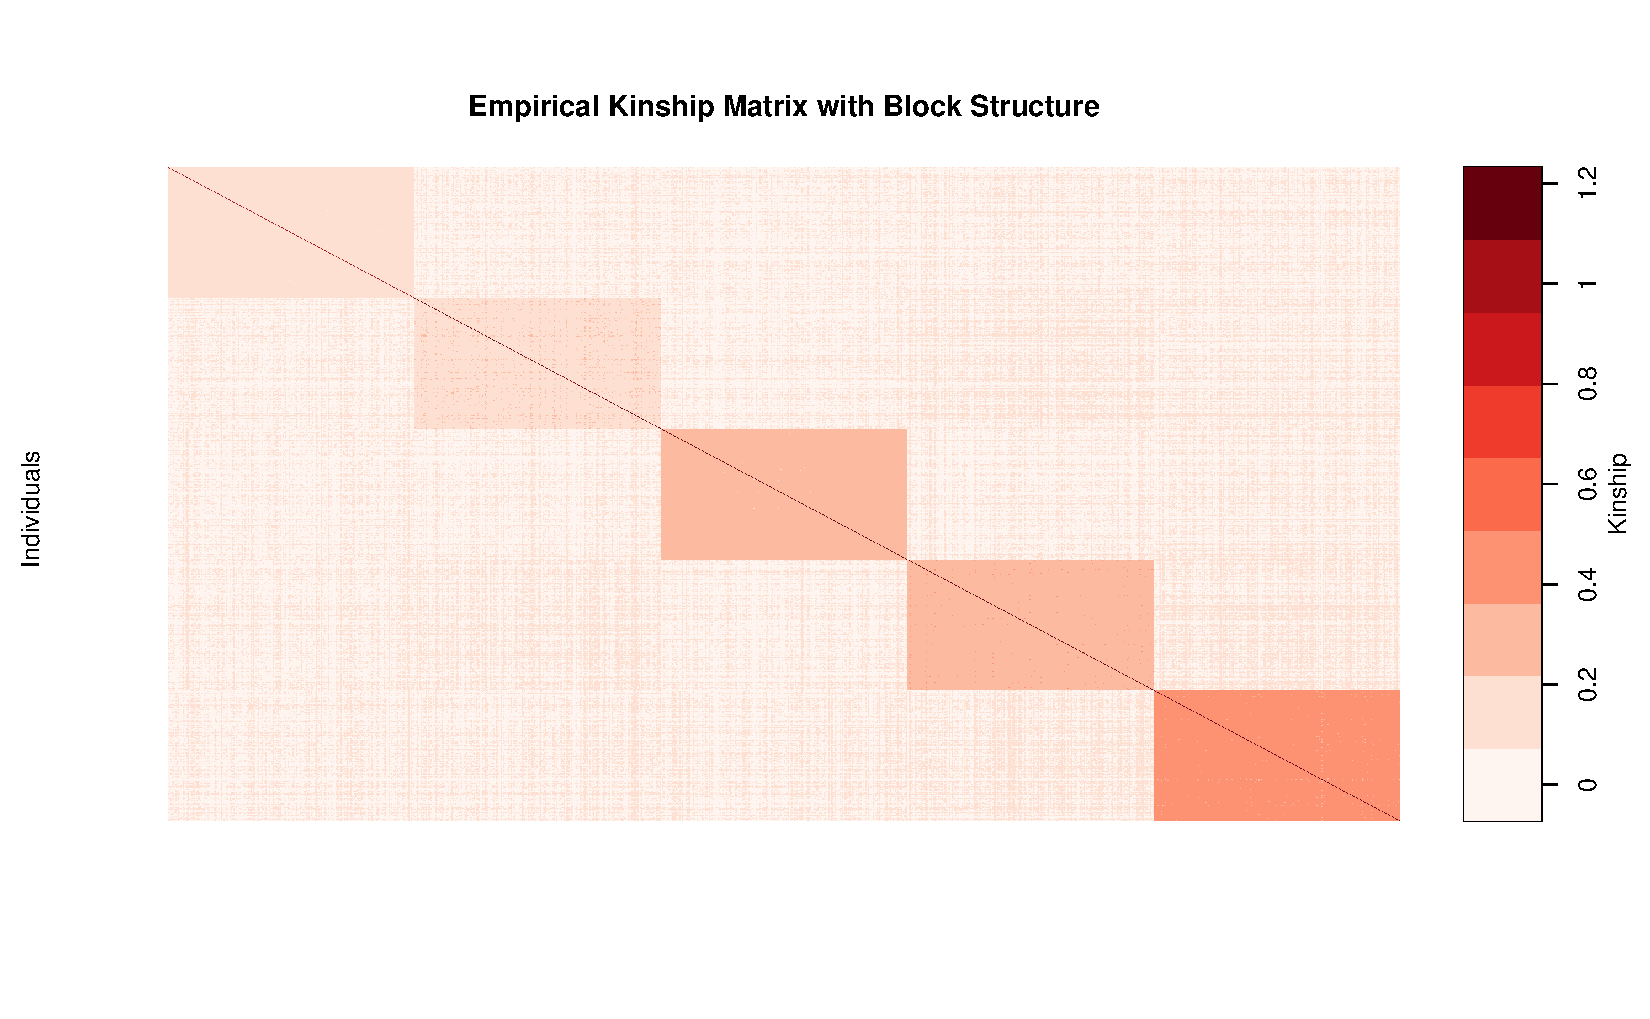
\includegraphics[width=1\linewidth]{figure/plot-kinship-sim-1} 

}

\caption[Empirical kinship matrices used in simulation studies]{Empirical kinship matrices used in simulation studies.}\label{fig:plot-kinship-sim}
\end{figure}


\end{knitrout}

\begin{knitrout}\scriptsize
\definecolor{shadecolor}{rgb}{0.969, 0.969, 0.969}\color{fgcolor}\begin{figure}[H]

{\centering 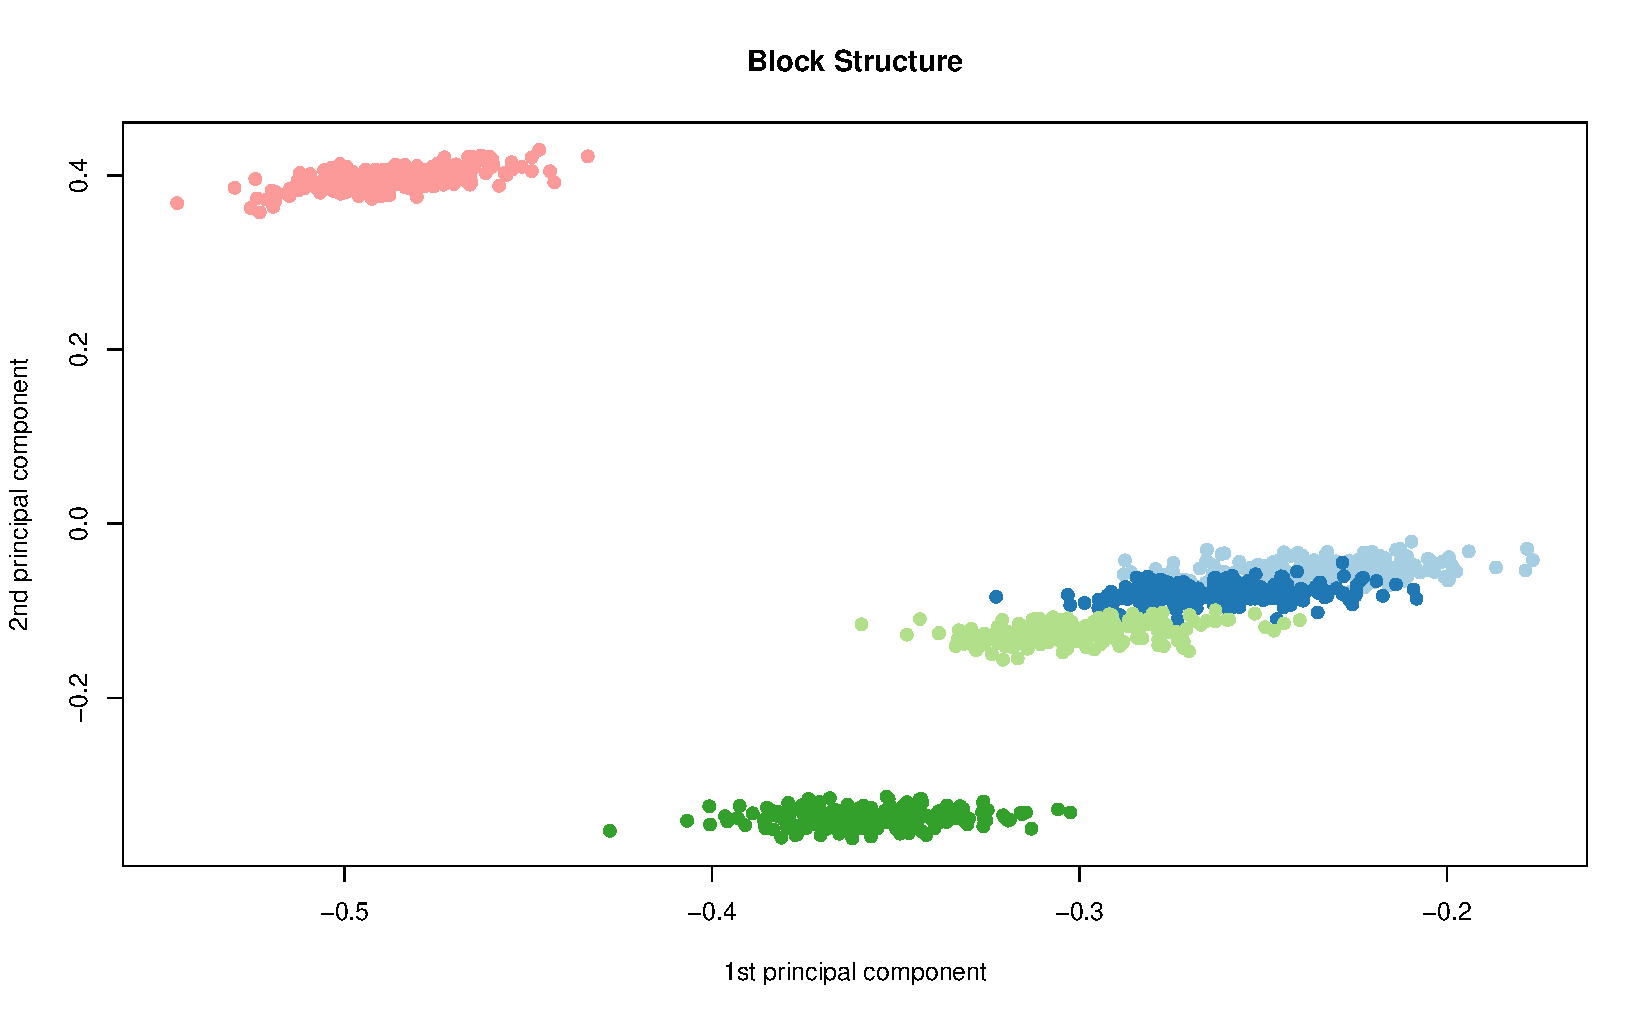
\includegraphics[width=1\linewidth]{figure/plot-pc-sim-1} 

}

\caption[First two principal component scores of the kinship matrix where each color represents one of the 5 simulated subpopulations]{First two principal component scores of the kinship matrix where each color represents one of the 5 simulated subpopulations. The first panel corresponds to 5 independent subpopulations, the second corresponds to a 1 dimensional geographical structure and the thrid panel corresponds to a circular geography.}\label{fig:plot-pc-sim}
\end{figure}


\end{knitrout}

need to add error variance formula for lasso. 

\subsection{Results}



\begin{knitrout}\scriptsize
\definecolor{shadecolor}{rgb}{0.969, 0.969, 0.969}\color{fgcolor}\begin{figure}[H]

{\centering 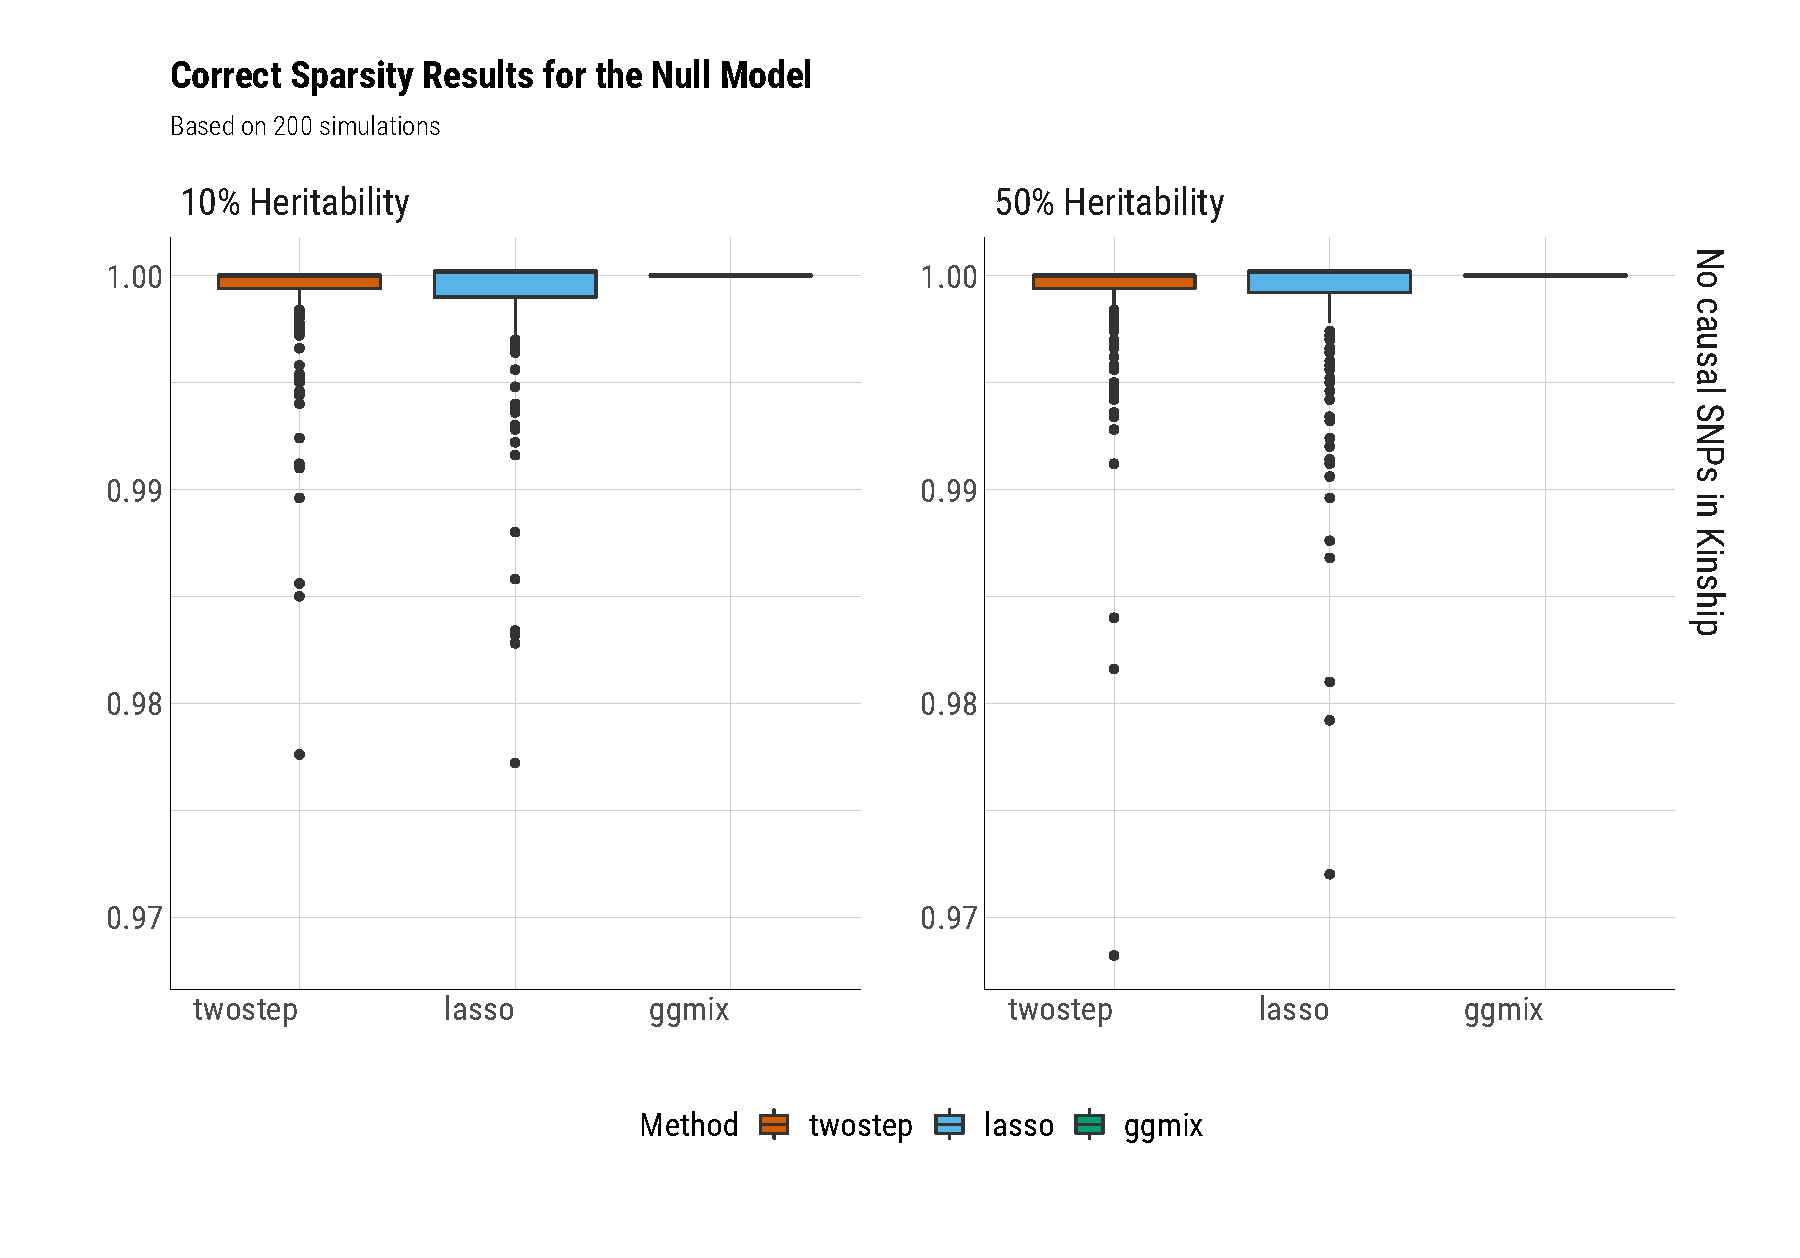
\includegraphics[width=1\linewidth]{figure/plot-correct-sparsity-sim-null-model-1} 

}

\caption[Boxplots of the correct sparsity from 200 simulations by heritability and number of causal SNPs that were included in the calculation of the kinship matrix for the null model]{Boxplots of the correct sparsity from 200 simulations by heritability and number of causal SNPs that were included in the calculation of the kinship matrix for the null model.}\label{fig:plot-correct-sparsity-sim-null-model}
\end{figure}


\end{knitrout}

\begin{knitrout}\scriptsize
\definecolor{shadecolor}{rgb}{0.969, 0.969, 0.969}\color{fgcolor}\begin{figure}[H]

{\centering 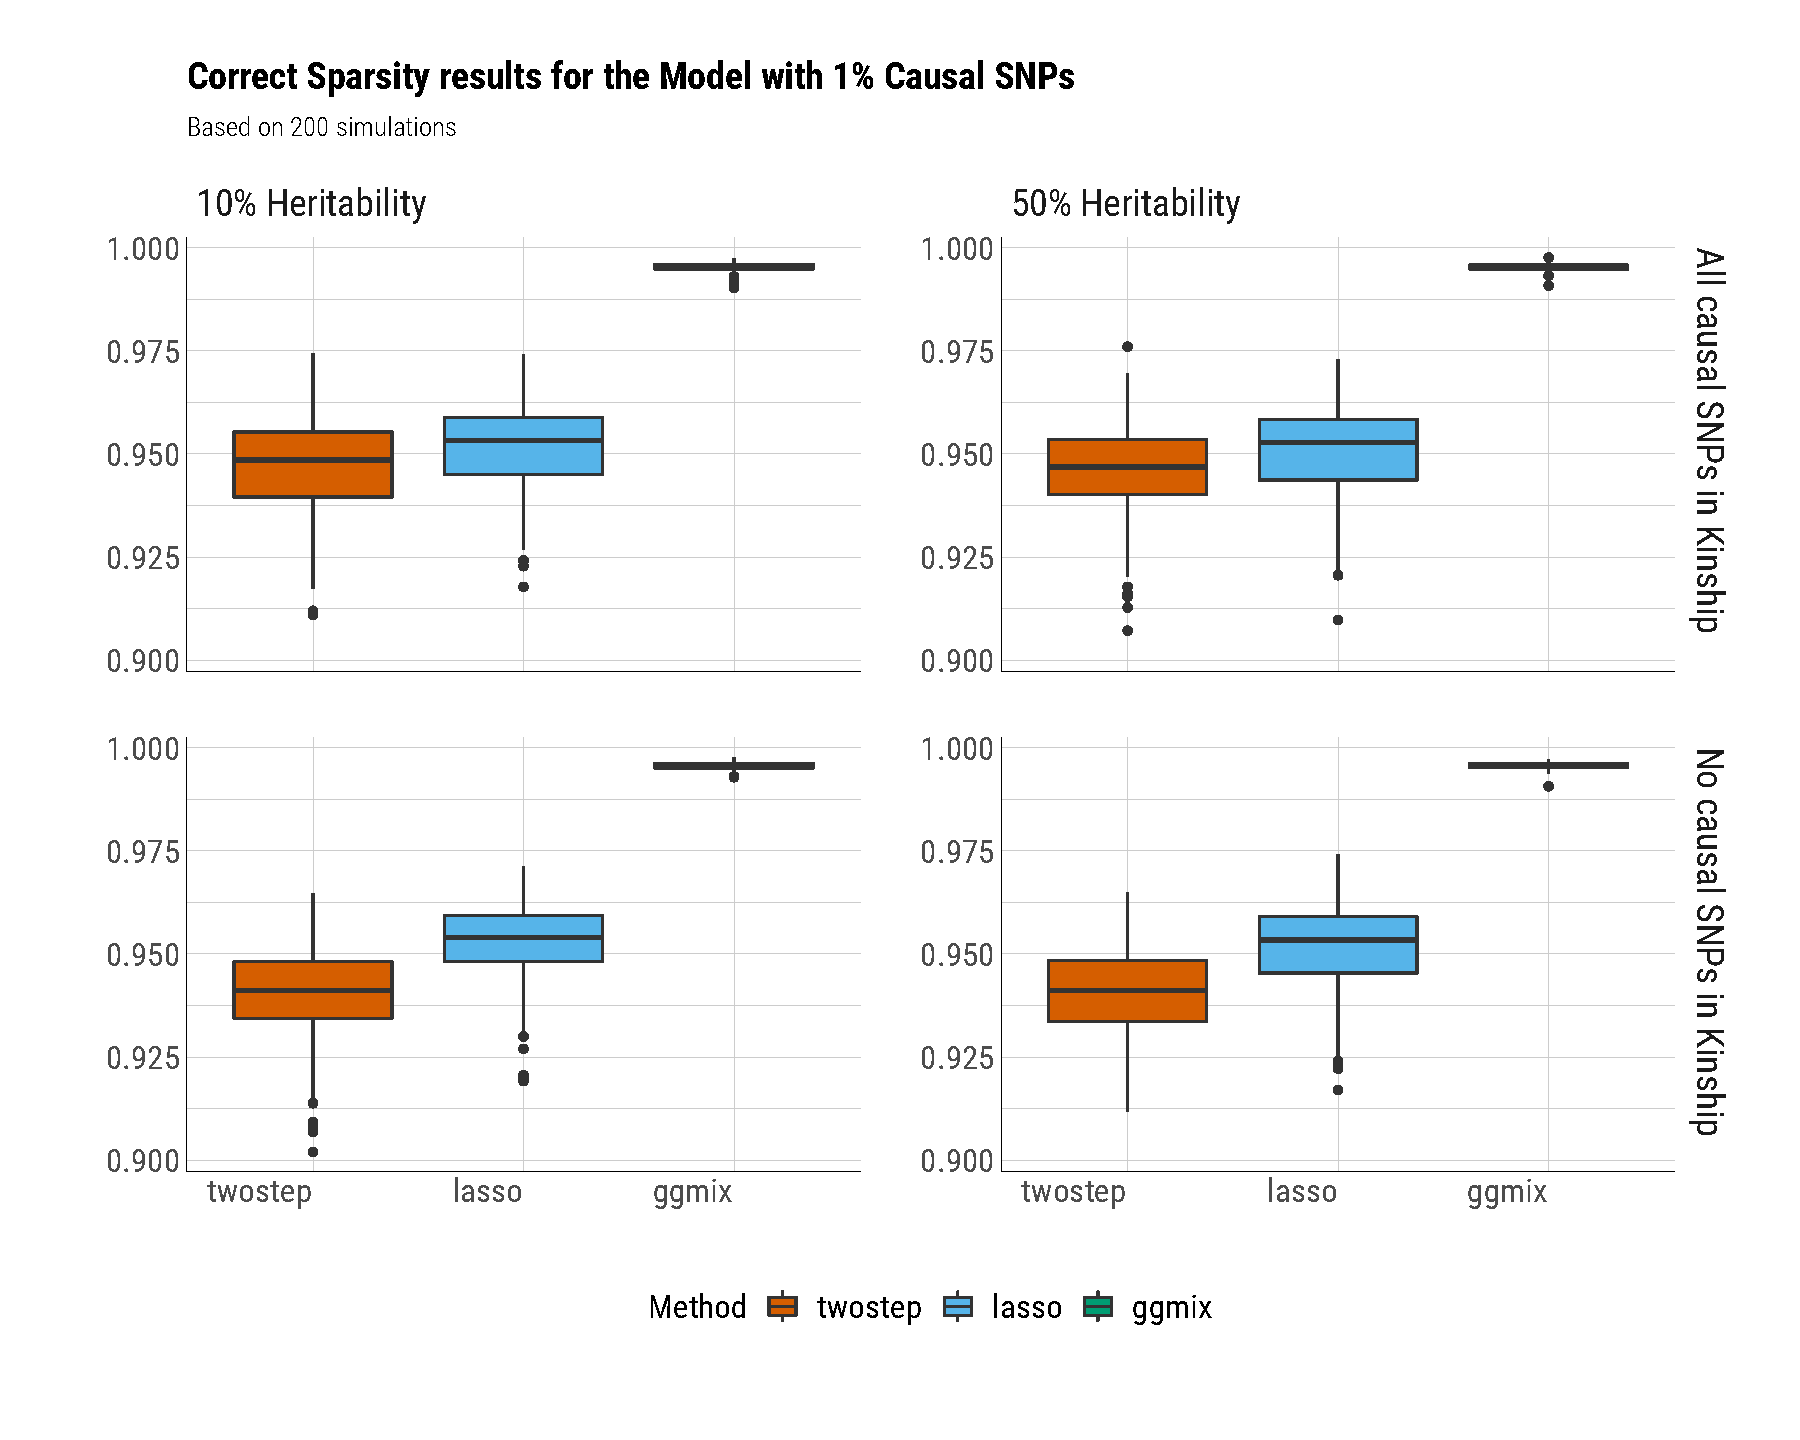
\includegraphics[width=1\linewidth]{figure/plot-correct-sparsity-sim-1p-causal-1} 

}

\caption[Boxplots of the correct sparsity from 200 simulations by heritability and number of causal SNPs that were included in the calculation of the kinship matrix for the model with 1\% causal SNPs]{Boxplots of the correct sparsity from 200 simulations by heritability and number of causal SNPs that were included in the calculation of the kinship matrix for the model with 1\% causal SNPs}\label{fig:plot-correct-sparsity-sim-1p-causal}
\end{figure}


\end{knitrout}


\begin{knitrout}\scriptsize
\definecolor{shadecolor}{rgb}{0.969, 0.969, 0.969}\color{fgcolor}\begin{figure}[H]

{\centering 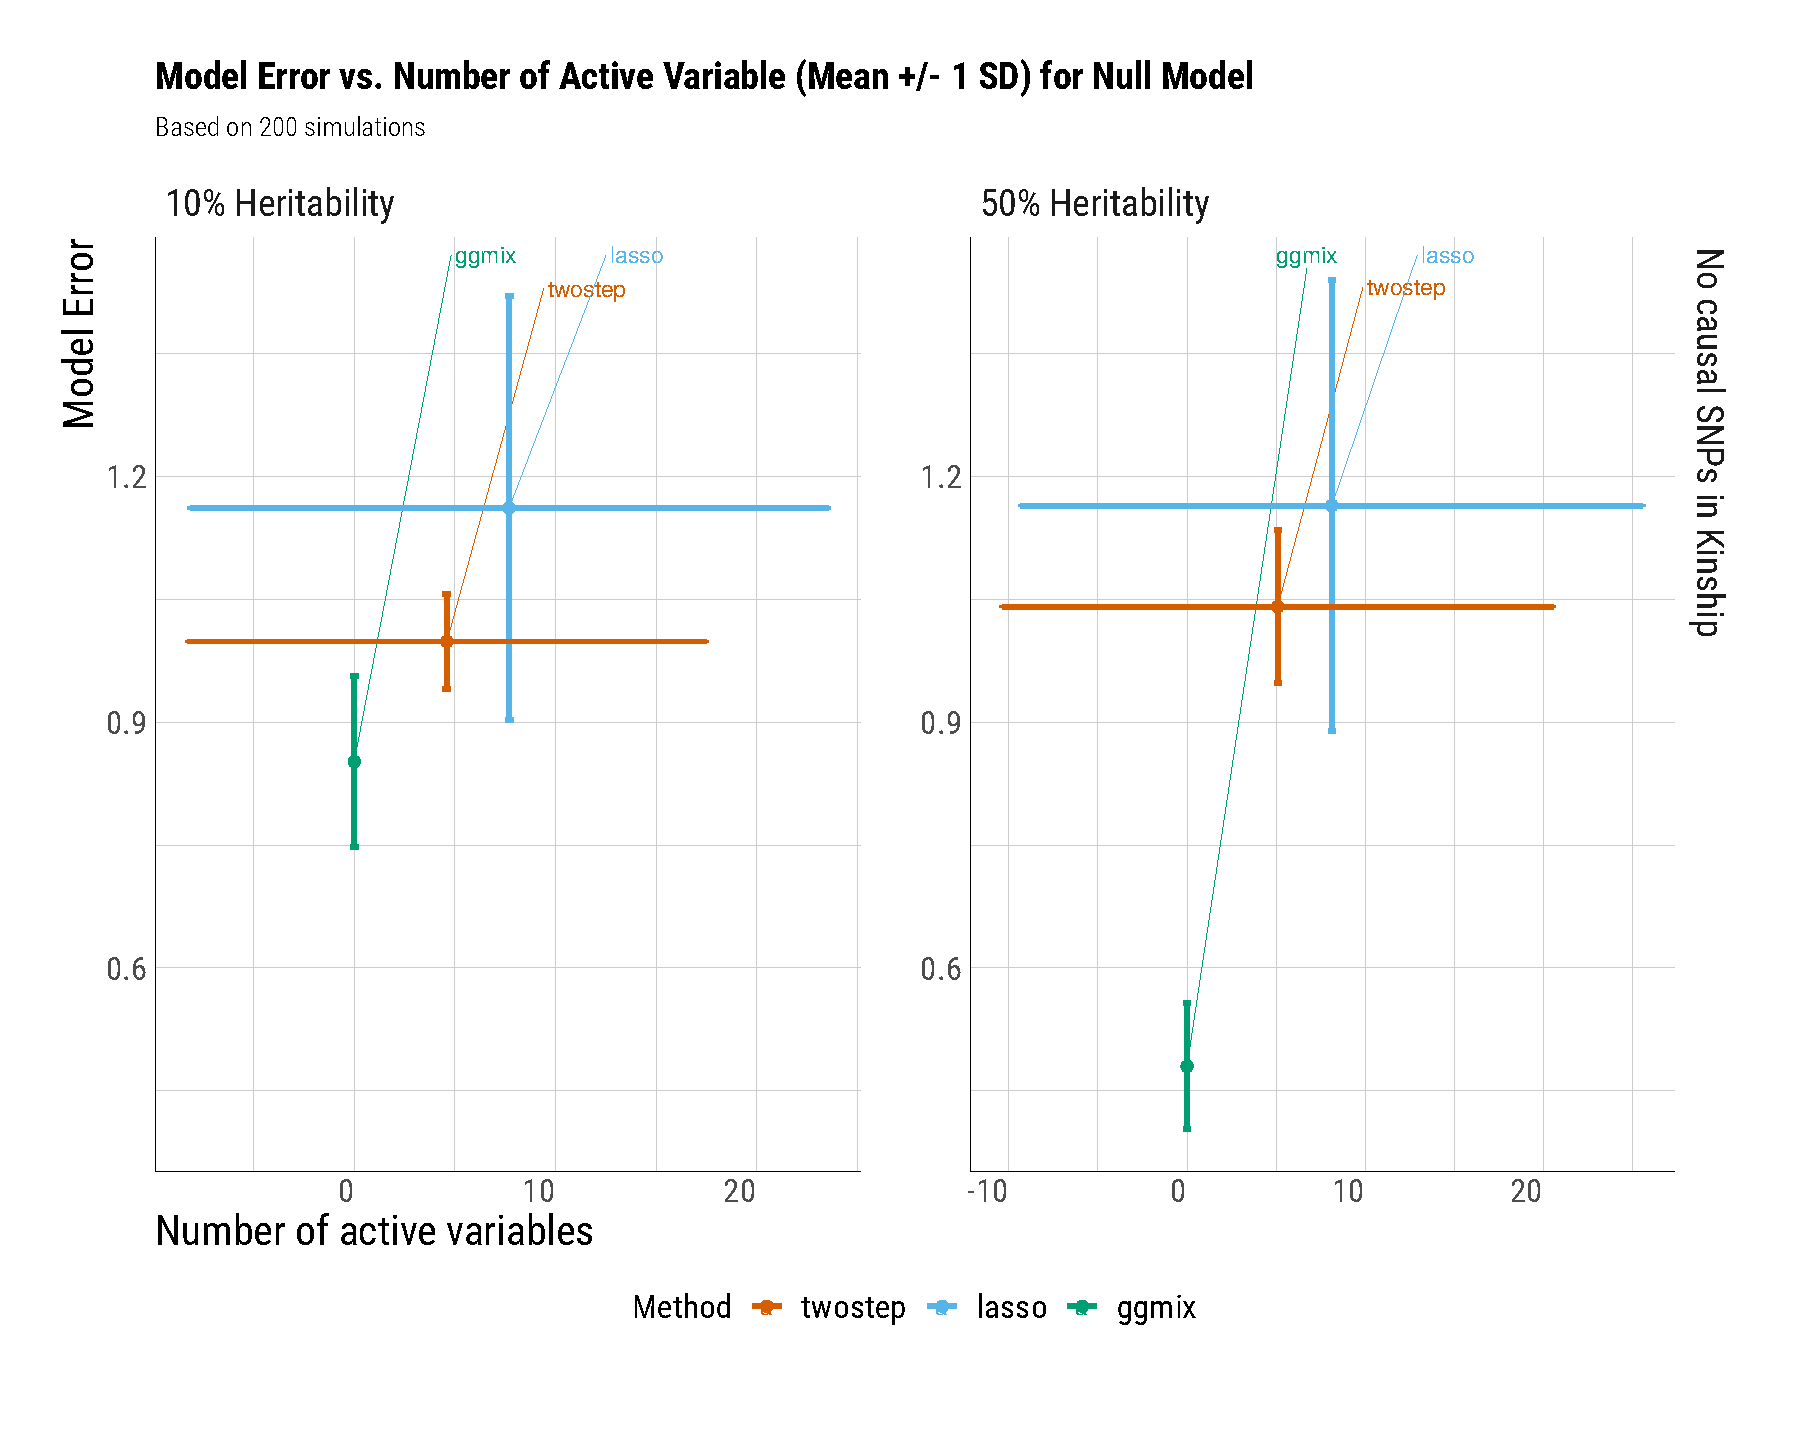
\includegraphics[width=1\linewidth]{figure/plot-me-nactive-sim-null-1} 

}

\caption[Model error vs number of active variables results for the null model]{Model error vs number of active variables results for the null model.}\label{fig:plot-me-nactive-sim-null}
\end{figure}


\end{knitrout}

\begin{knitrout}\scriptsize
\definecolor{shadecolor}{rgb}{0.969, 0.969, 0.969}\color{fgcolor}\begin{figure}[H]

{\centering 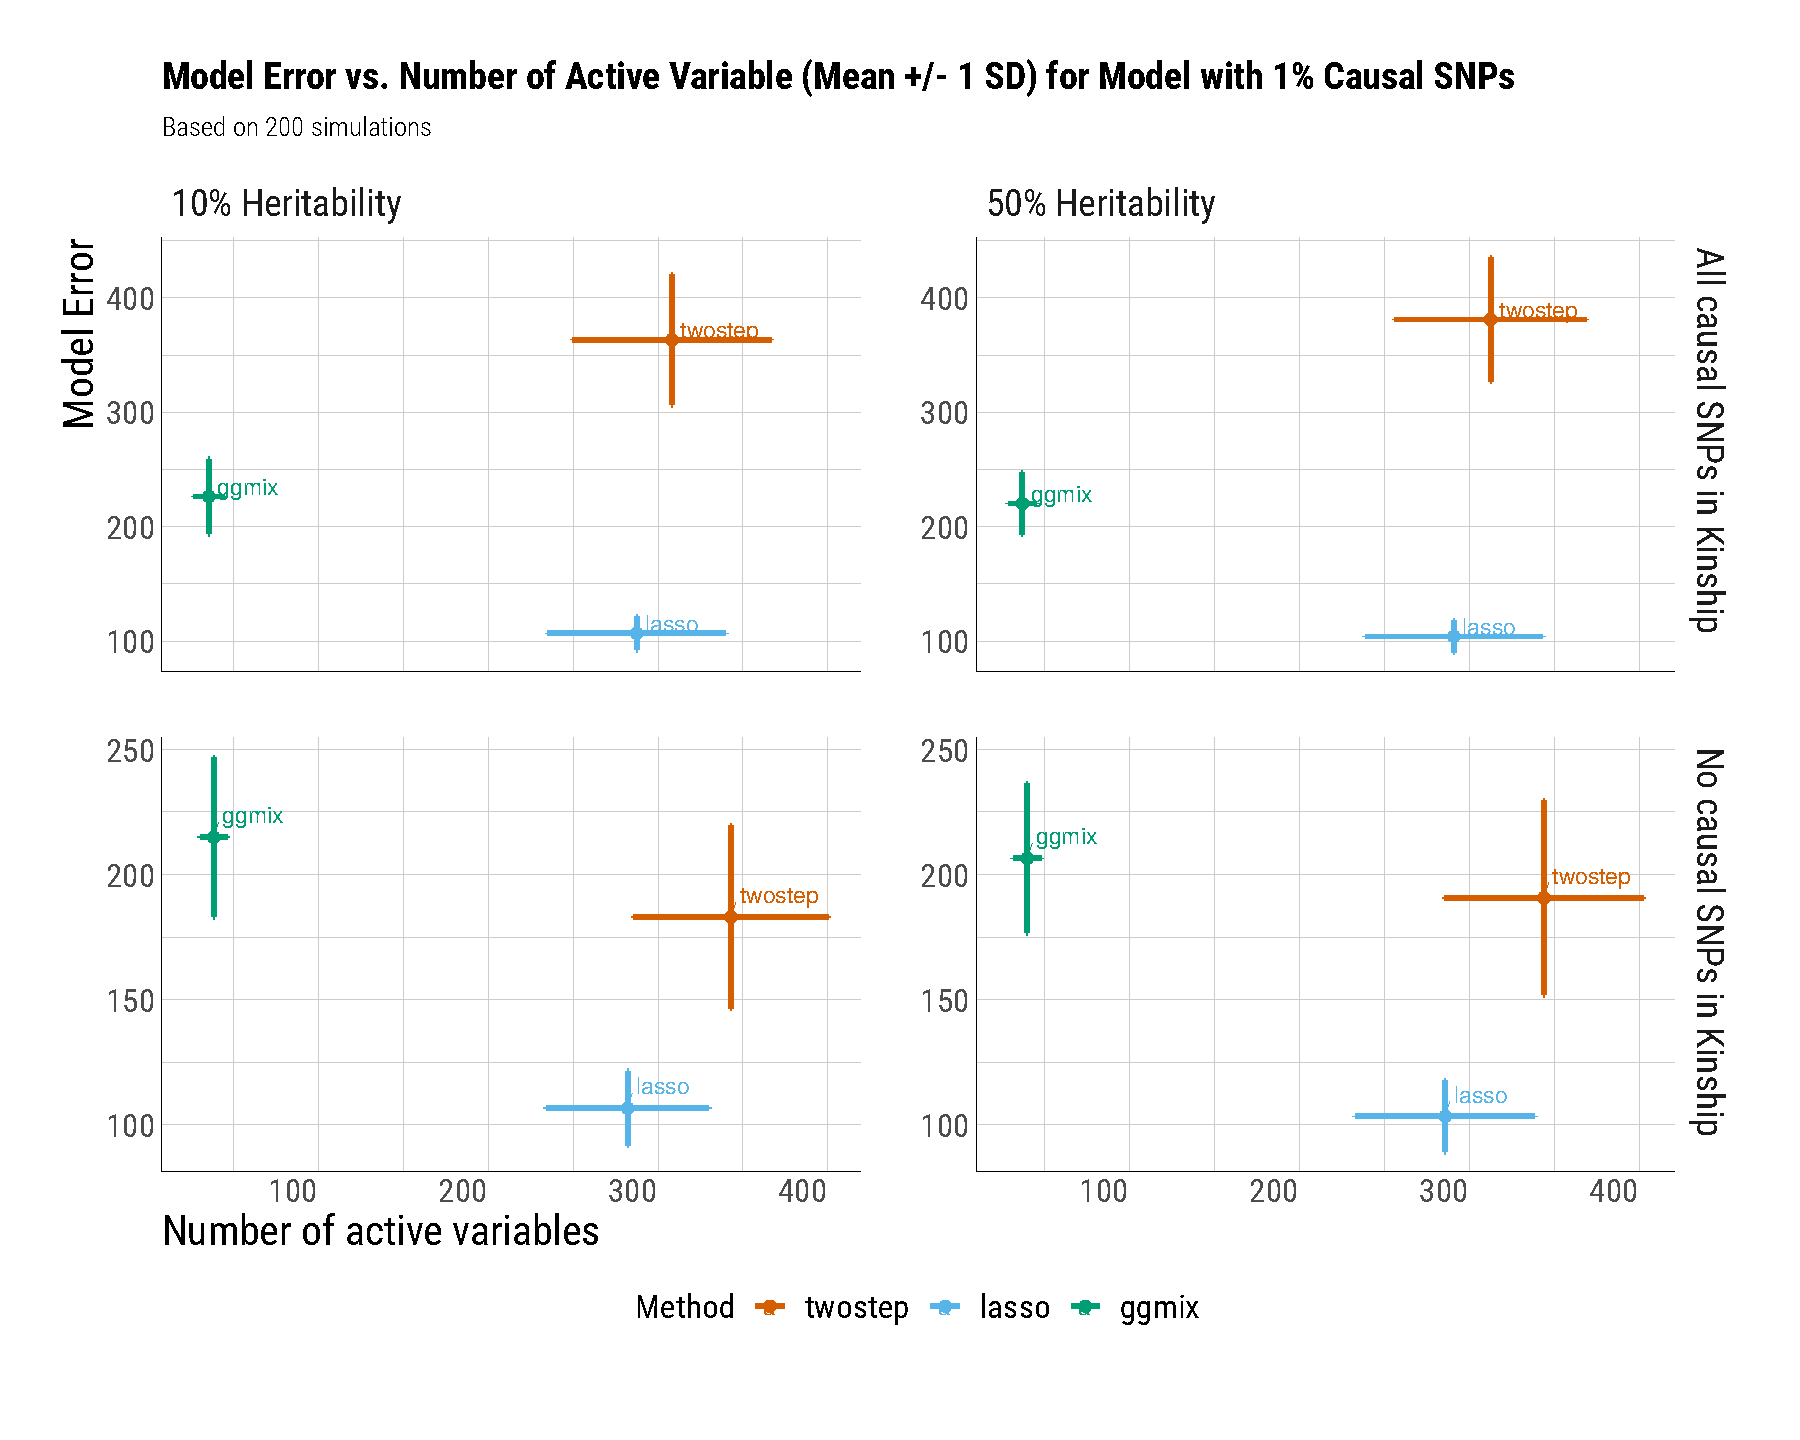
\includegraphics[width=1\linewidth]{figure/plot-me-nactive-sim-1p-causal-1} 

}

\caption[Model error vs number of active variables results for the model with 1\% causal SNPs]{Model error vs number of active variables results for the model with 1\% causal SNPs.}\label{fig:plot-me-nactive-sim-1p-causal}
\end{figure}


\end{knitrout}


\begin{knitrout}\scriptsize
\definecolor{shadecolor}{rgb}{0.969, 0.969, 0.969}\color{fgcolor}\begin{figure}[H]

{\centering 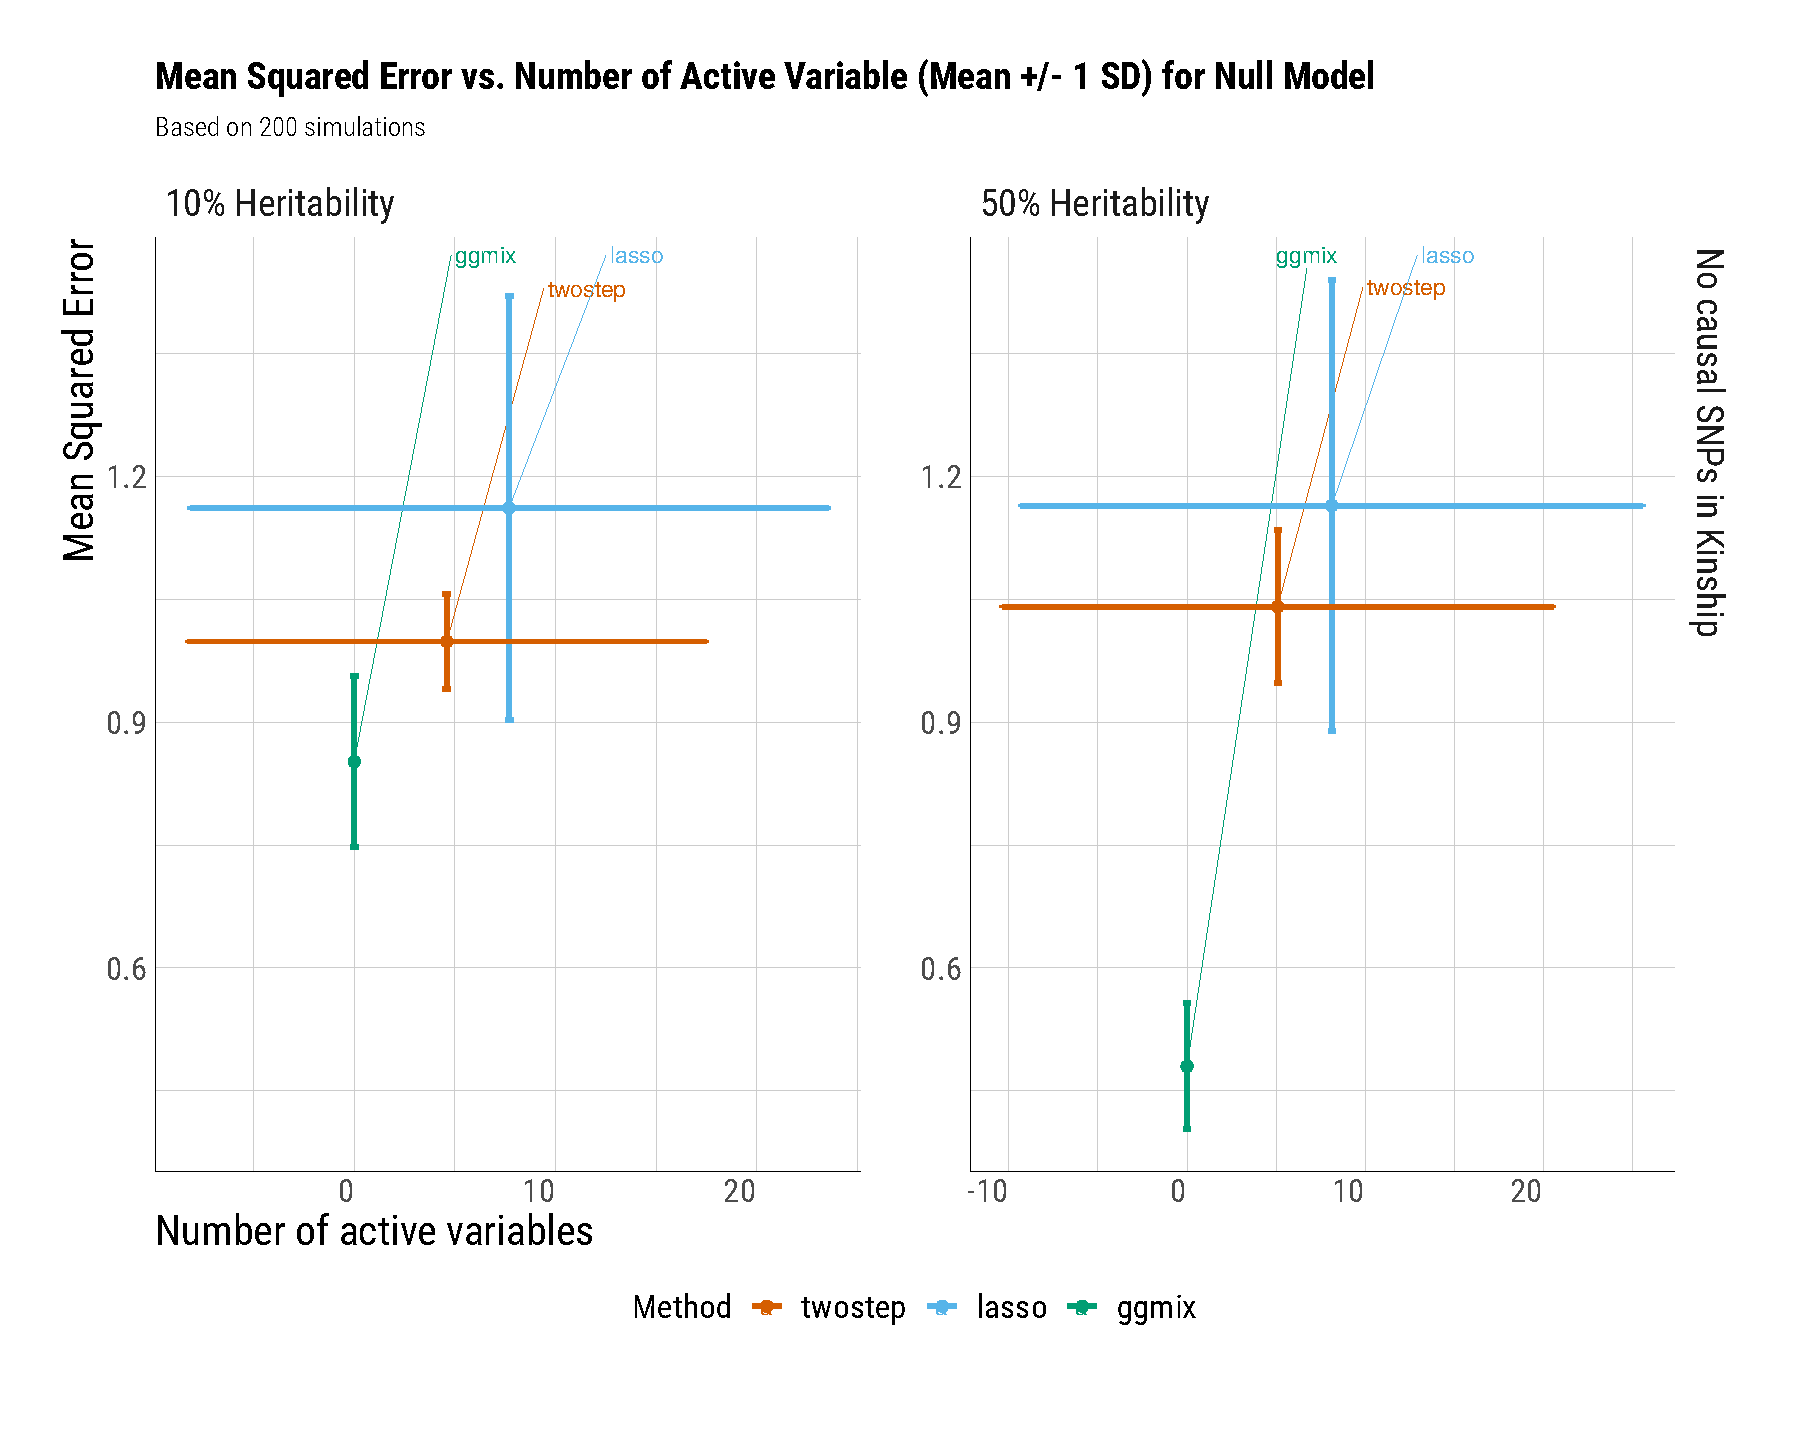
\includegraphics[width=1\linewidth]{figure/plot-mse-nactive-sim-null-1} 

}

\caption[Mean squared error vs number of active variables results for the null model]{Mean squared error vs number of active variables results for the null model.}\label{fig:plot-mse-nactive-sim-null}
\end{figure}


\end{knitrout}

\begin{knitrout}\scriptsize
\definecolor{shadecolor}{rgb}{0.969, 0.969, 0.969}\color{fgcolor}\begin{figure}[H]

{\centering 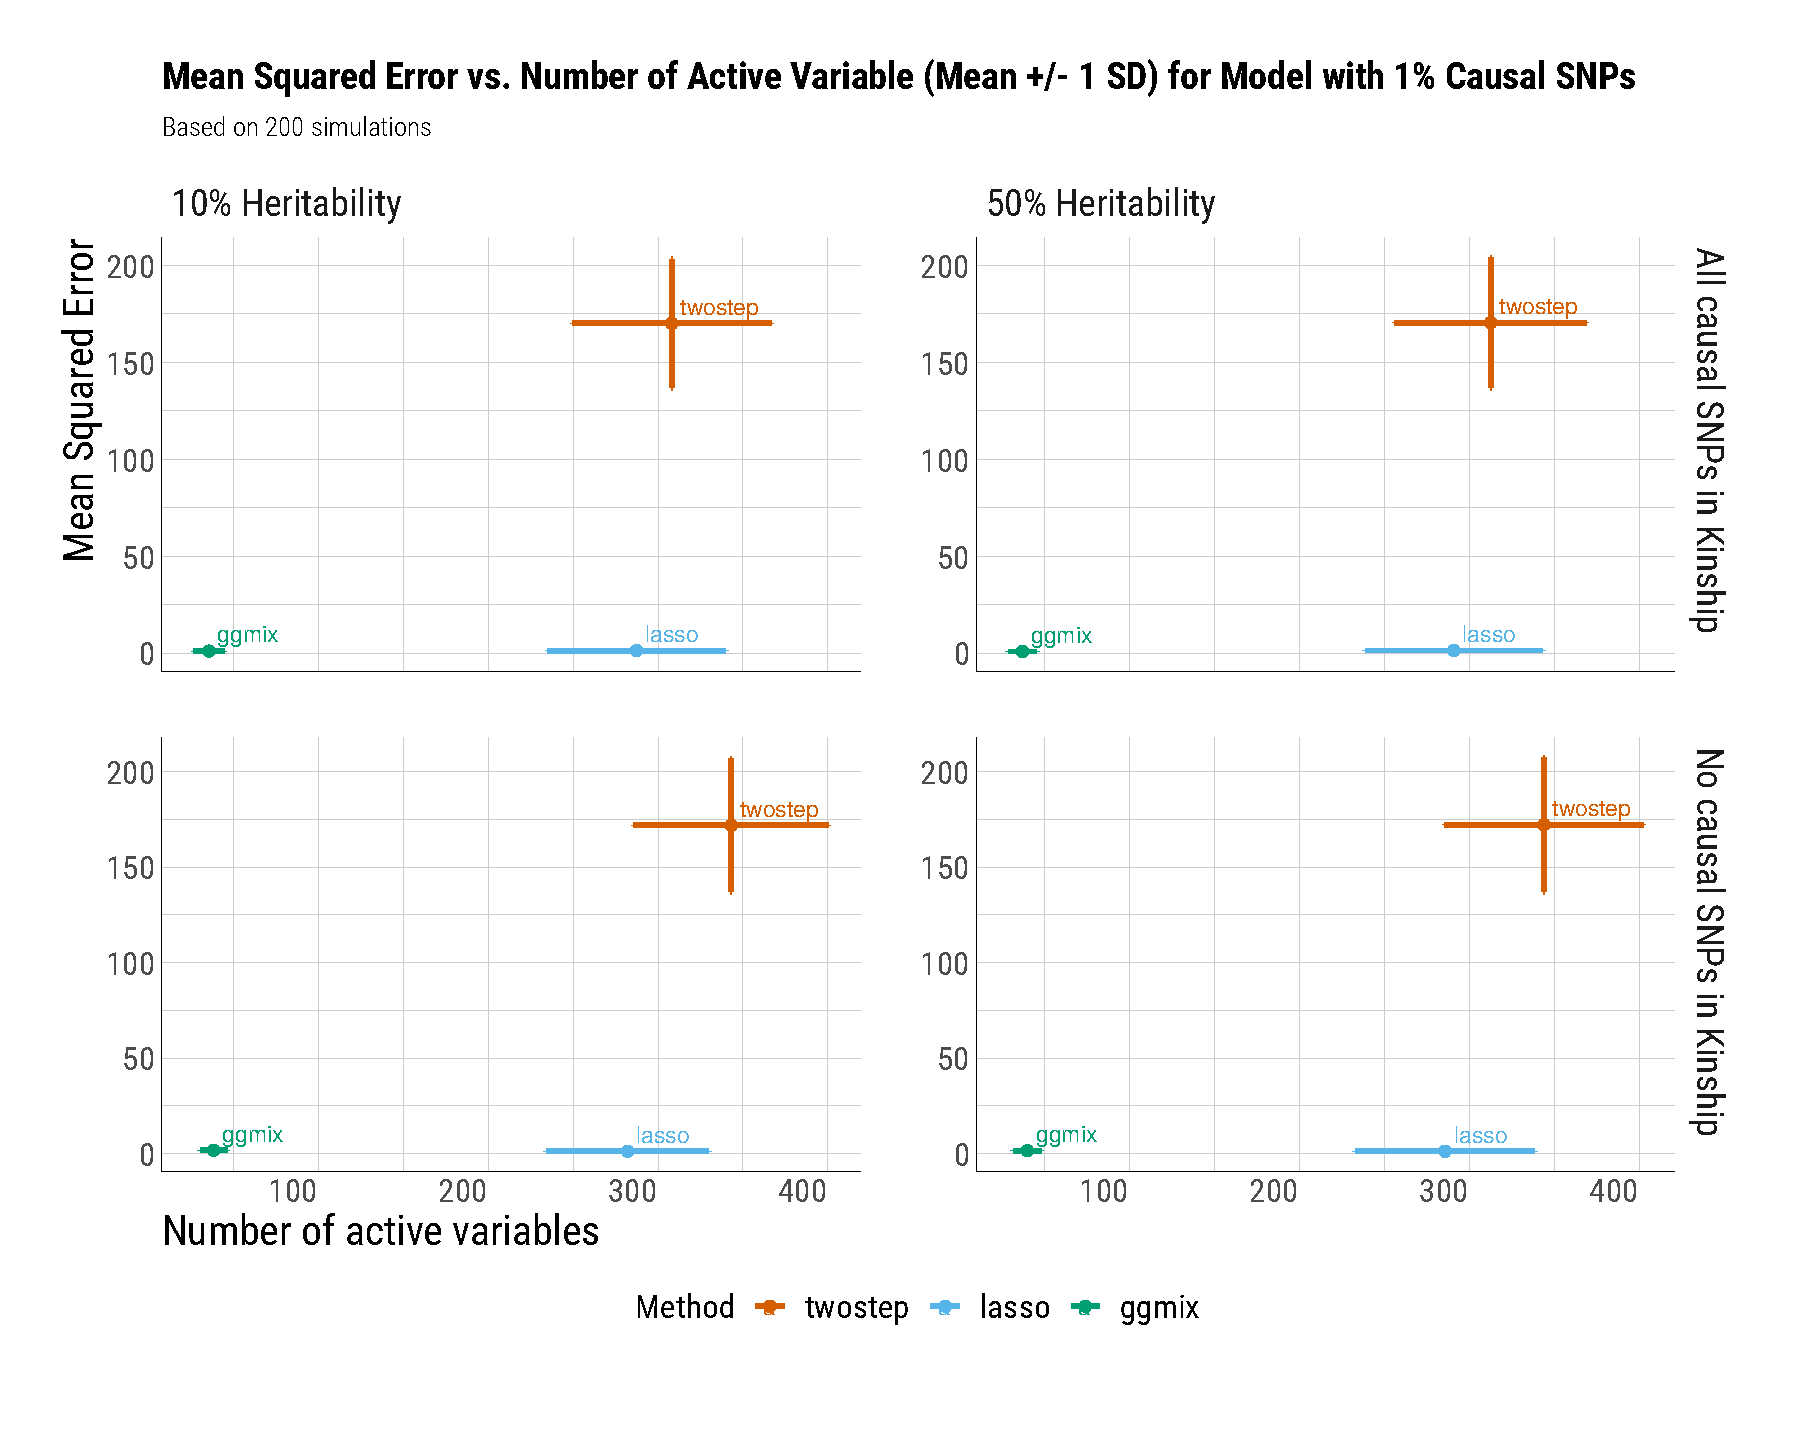
\includegraphics[width=1\linewidth]{figure/plot-mse-nactive-sim-1p-causal-1} 

}

\caption[Mean squared error vs number of active variables results for the model with 1\% causal SNPs]{Mean squared error vs number of active variables results for the model with 1\% causal SNPs.}\label{fig:plot-mse-nactive-sim-1p-causal}
\end{figure}


\end{knitrout}


\begin{knitrout}\scriptsize
\definecolor{shadecolor}{rgb}{0.969, 0.969, 0.969}\color{fgcolor}\begin{figure}[H]

{\centering 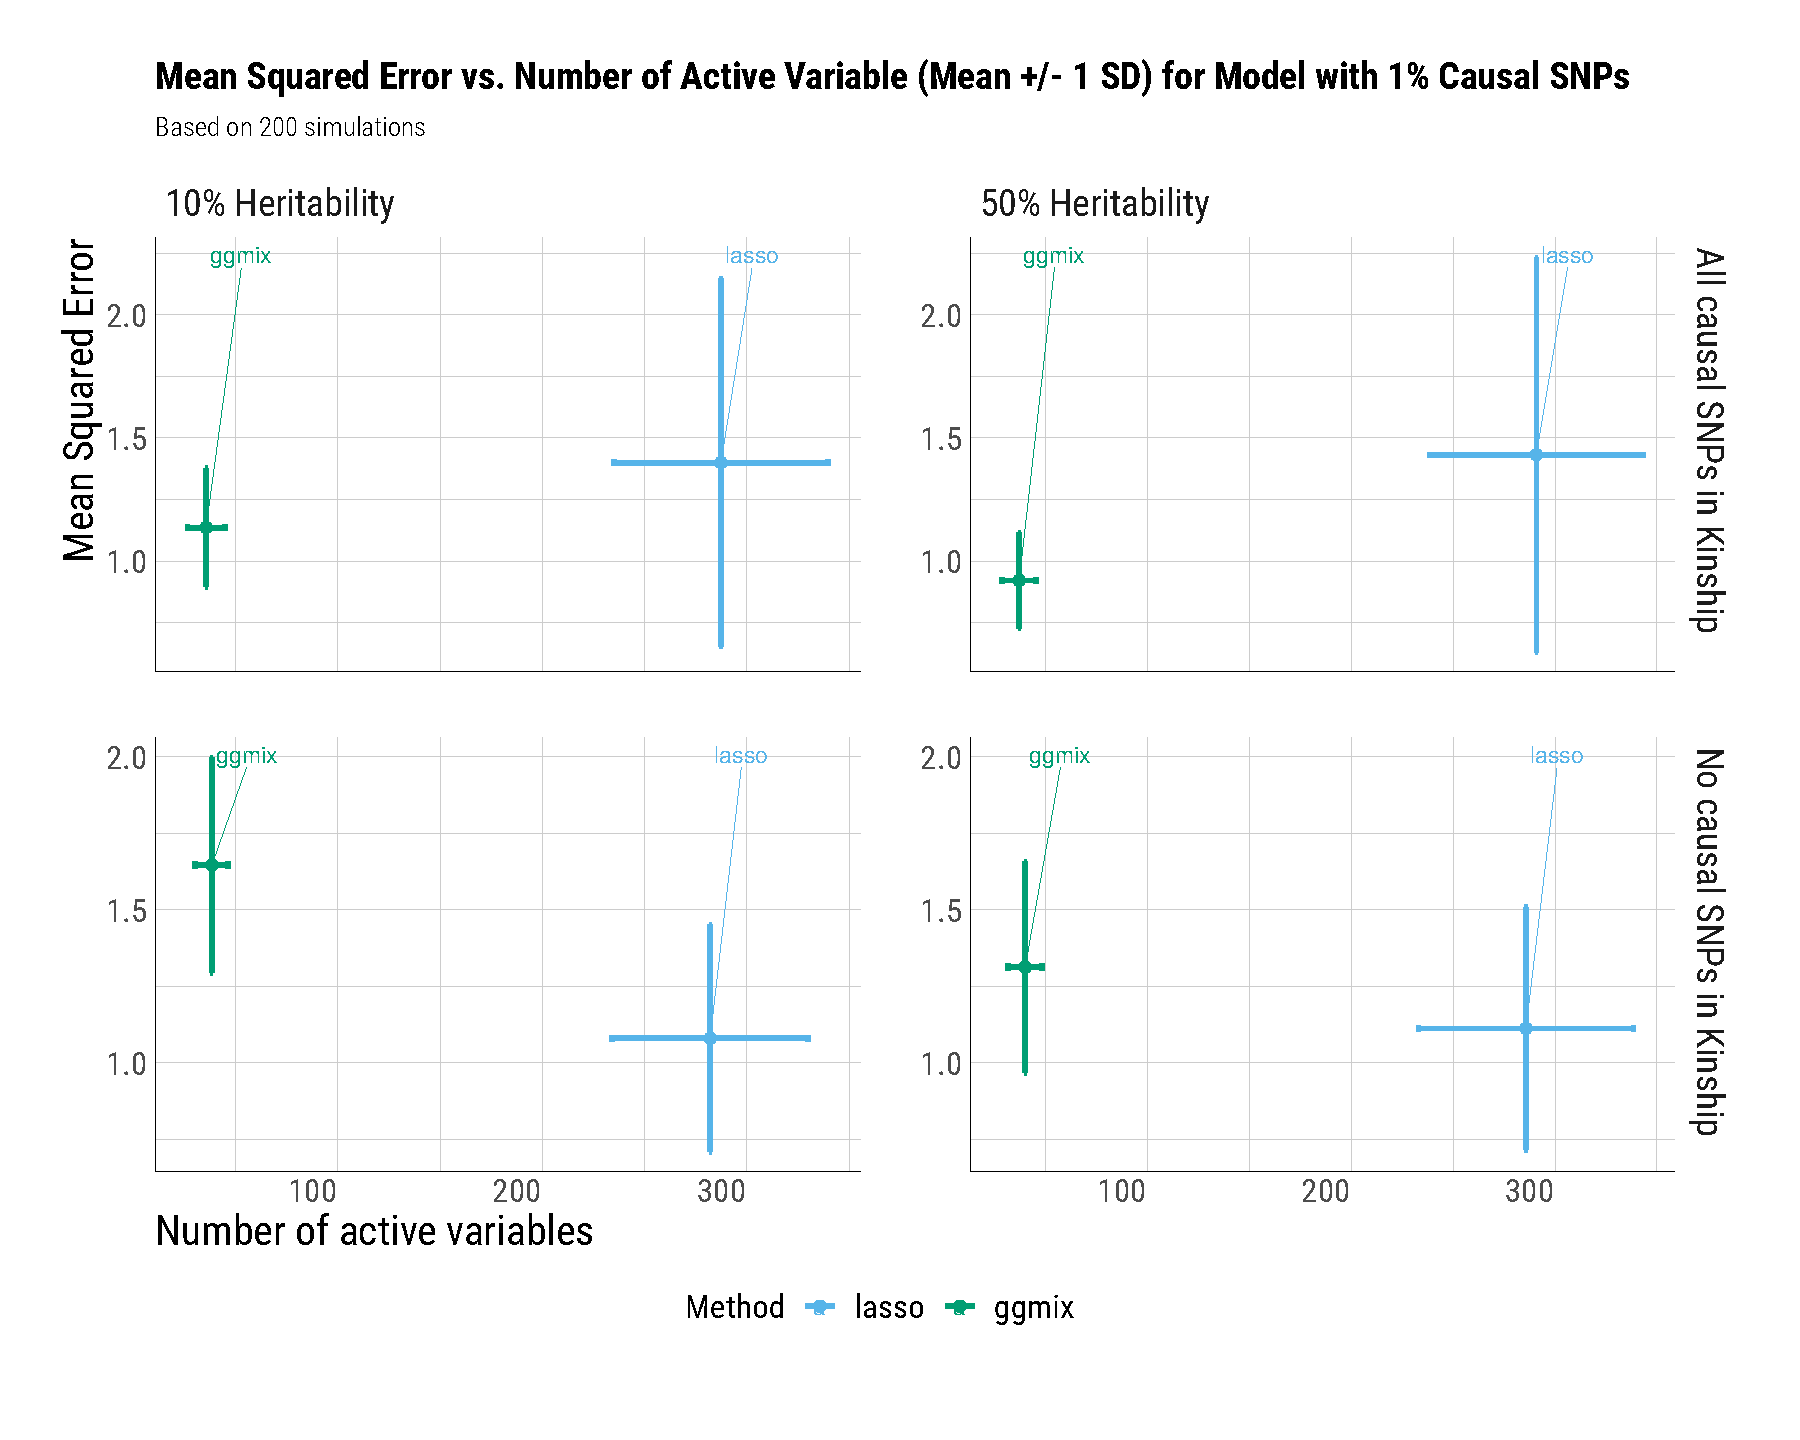
\includegraphics[width=1\linewidth]{figure/plot-mse-nactive-sim-1p-causal-zoom-in-1} 

}

\caption[Mean squared error vs number of active variables results for 1\% causal SNPs for ggmix and lasso]{Mean squared error vs number of active variables results for 1\% causal SNPs for ggmix and lasso.}\label{fig:plot-mse-nactive-sim-1p-causal-zoom-in}
\end{figure}


\end{knitrout}


\begin{knitrout}\scriptsize
\definecolor{shadecolor}{rgb}{0.969, 0.969, 0.969}\color{fgcolor}\begin{figure}[H]

{\centering 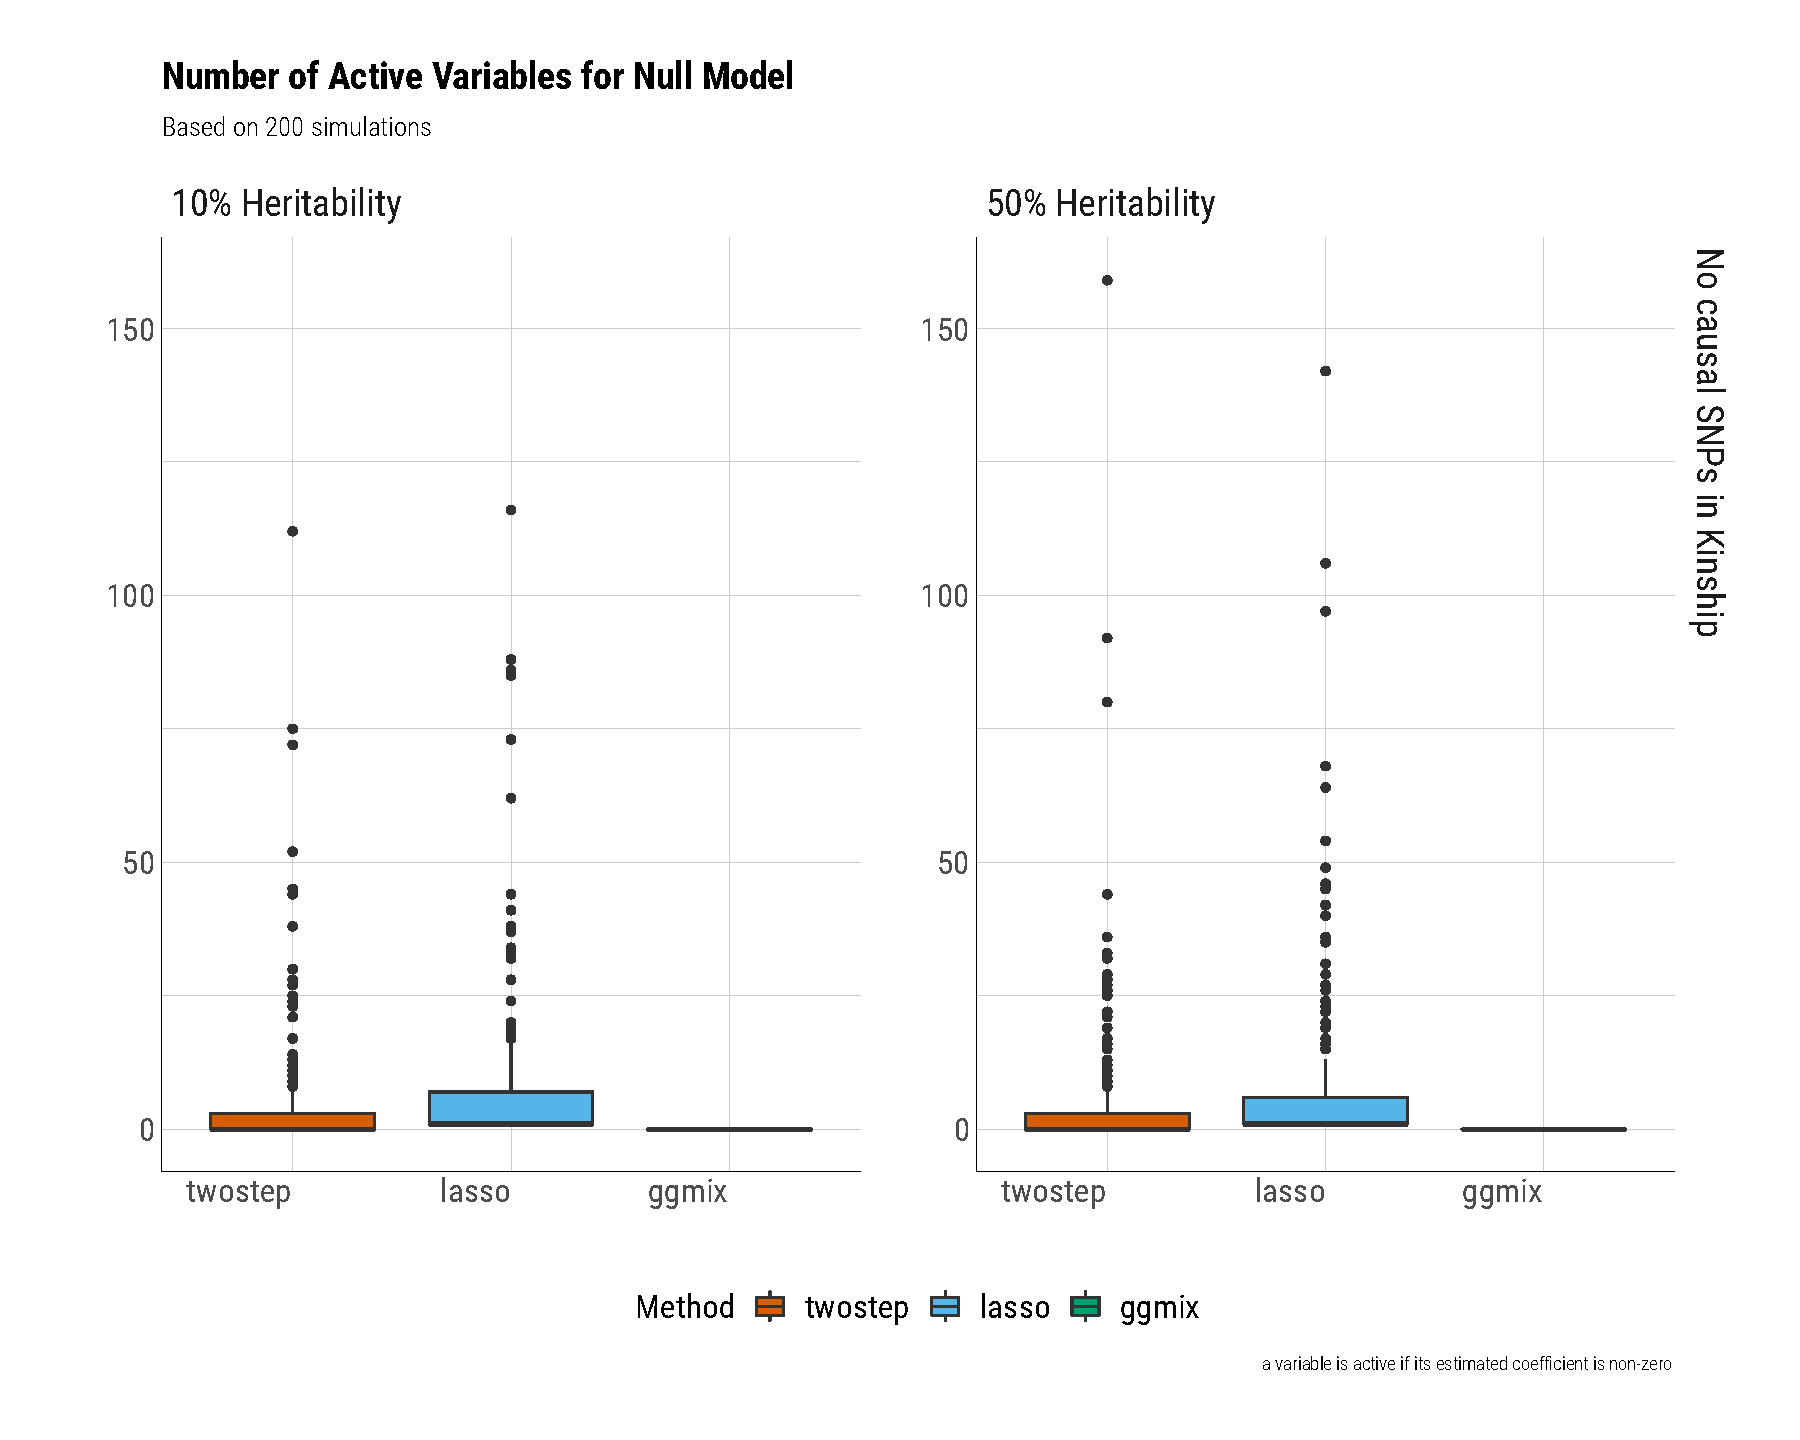
\includegraphics[width=1\linewidth]{figure/plot-nactive-sim-null-model-1} 

}

\caption[Boxplots of the number of active variables from 200 simulations by kinship geography and number of causal SNPs that were included in the calculation of the kinship matrix]{Boxplots of the number of active variables from 200 simulations by kinship geography and number of causal SNPs that were included in the calculation of the kinship matrix.}\label{fig:plot-nactive-sim-null-model}
\end{figure}


\end{knitrout}

\begin{knitrout}\scriptsize
\definecolor{shadecolor}{rgb}{0.969, 0.969, 0.969}\color{fgcolor}\begin{figure}[H]

{\centering 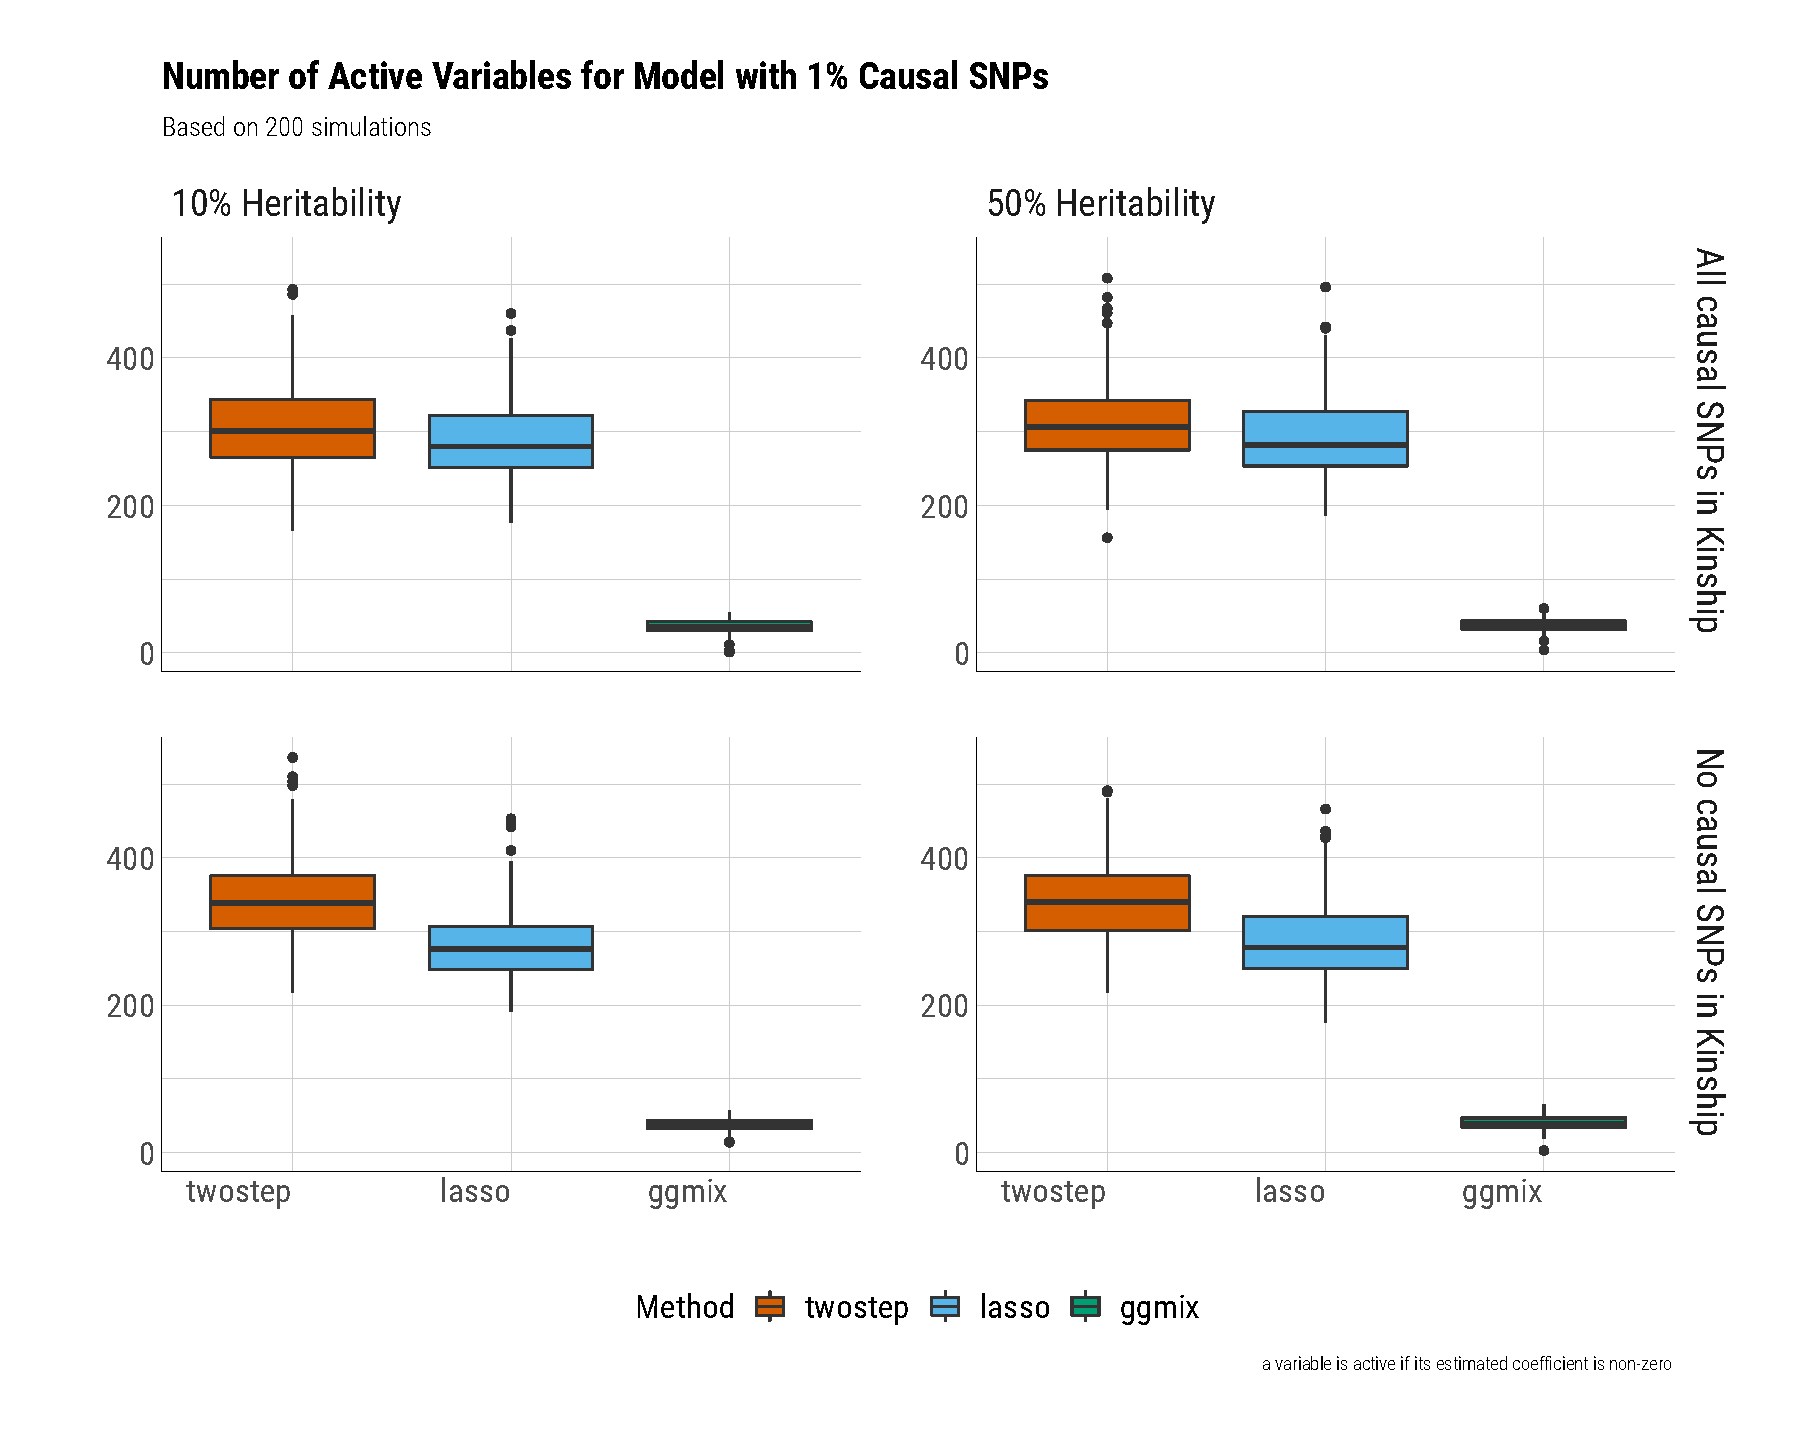
\includegraphics[width=1\linewidth]{figure/plot-nactive-sim-1p-causal-1} 

}

\caption[Boxplots of the number of active variables from 200 simulations by kinship geography and number of causal SNPs that were included in the calculation of the kinship matrix]{Boxplots of the number of active variables from 200 simulations by kinship geography and number of causal SNPs that were included in the calculation of the kinship matrix.}\label{fig:plot-nactive-sim-1p-causal}
\end{figure}


\end{knitrout}


\begin{knitrout}\scriptsize
\definecolor{shadecolor}{rgb}{0.969, 0.969, 0.969}\color{fgcolor}\begin{figure}[H]

{\centering 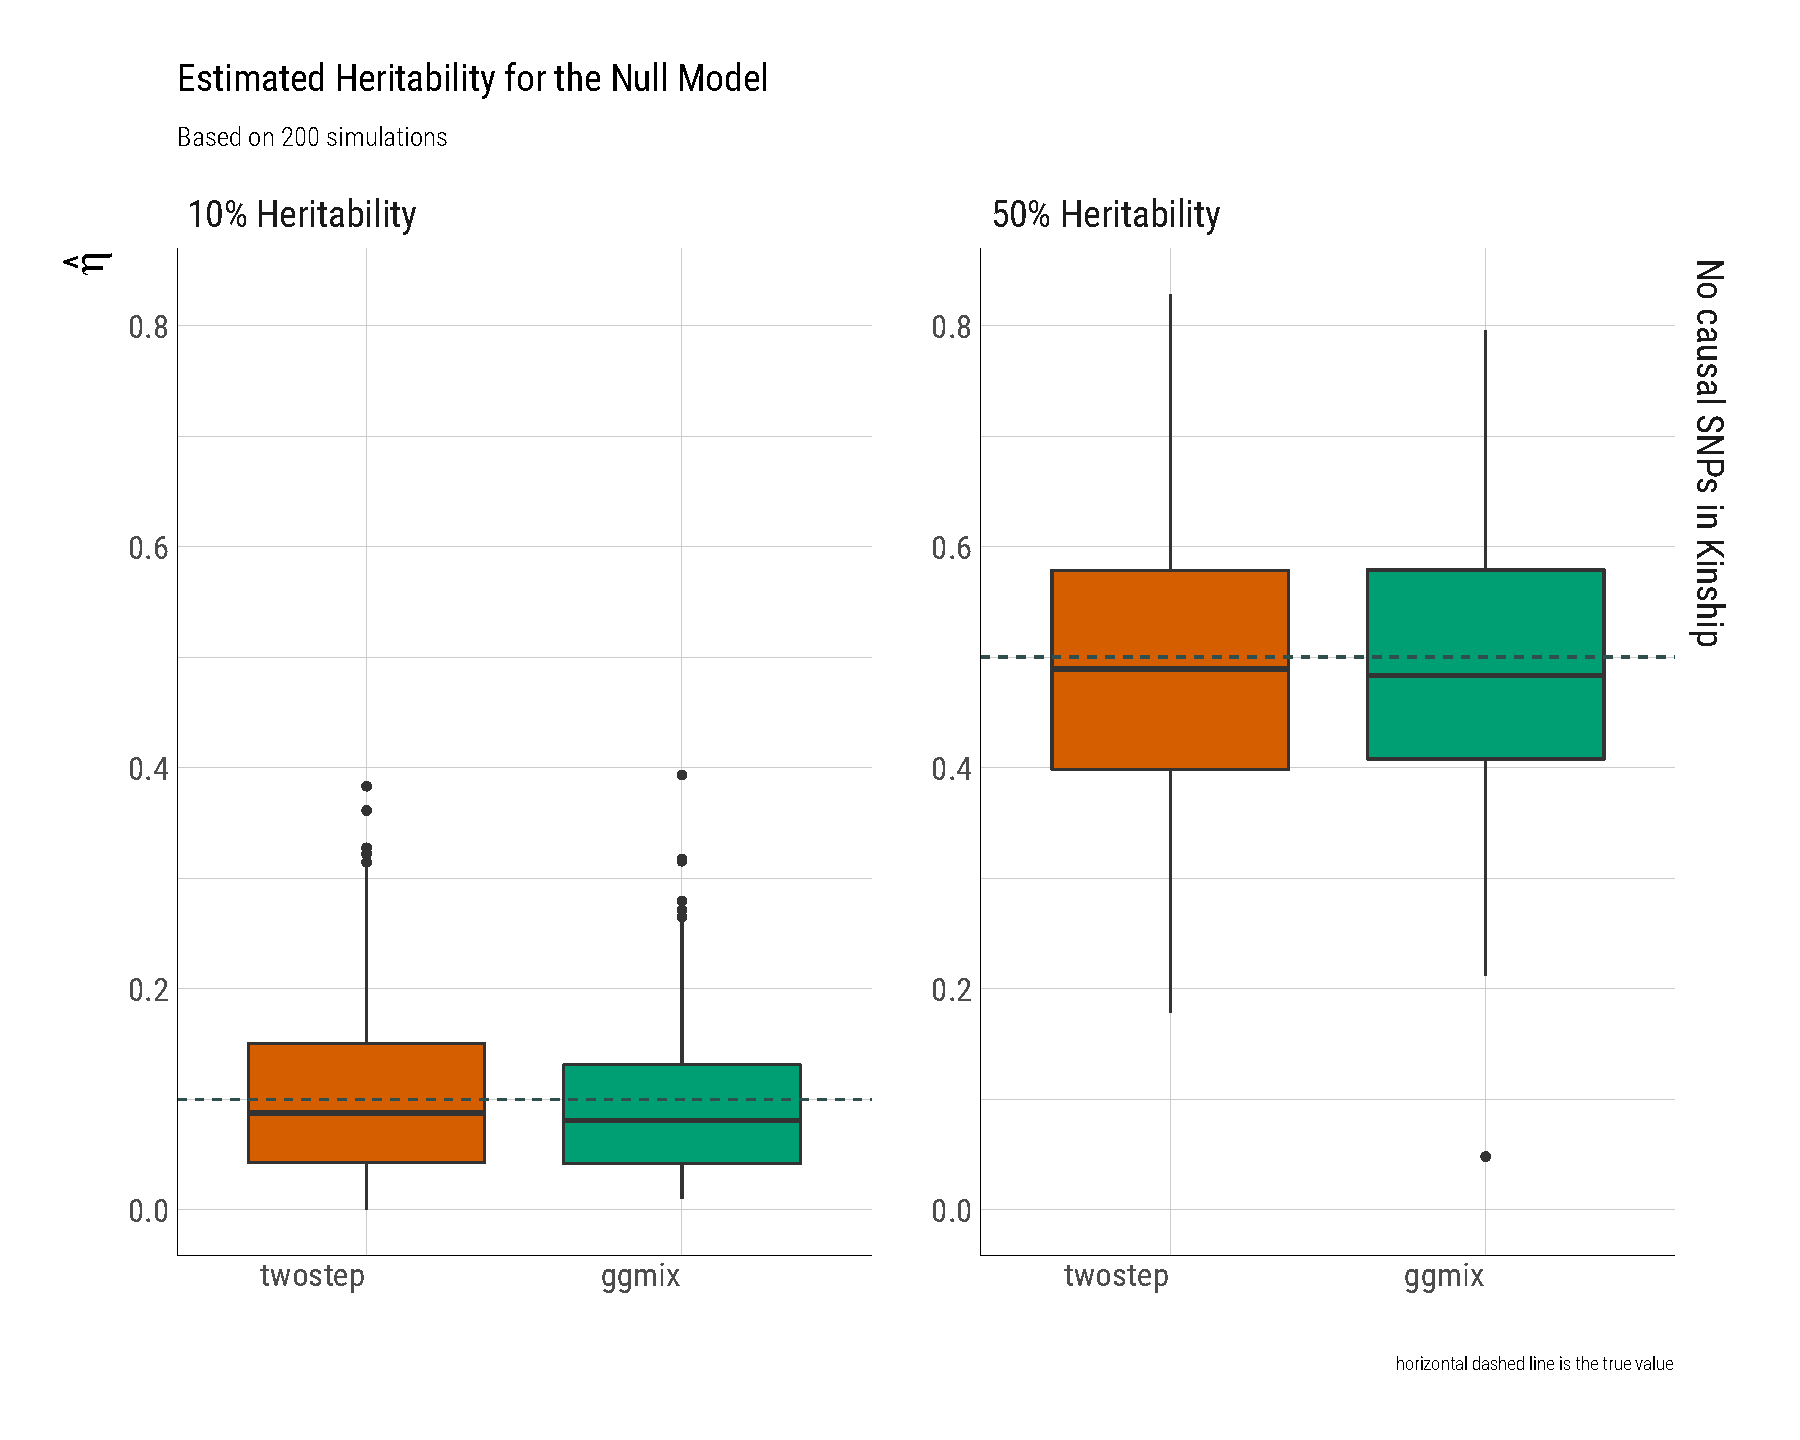
\includegraphics[width=1\linewidth]{figure/plot-eta-sim-null-model-1} 

}

\caption[Boxplot of $\hat{\eta}$ in the \texttt{ggmix} model from 200 simulations by kinship geography and number of causal SNPs that were included in the calculation of the kinship matrix]{Boxplot of $\hat{\eta}$ in the \texttt{ggmix} model from 200 simulations by kinship geography and number of causal SNPs that were included in the calculation of the kinship matrix.}\label{fig:plot-eta-sim-null-model}
\end{figure}


\end{knitrout}


\begin{knitrout}\scriptsize
\definecolor{shadecolor}{rgb}{0.969, 0.969, 0.969}\color{fgcolor}\begin{figure}[H]

{\centering 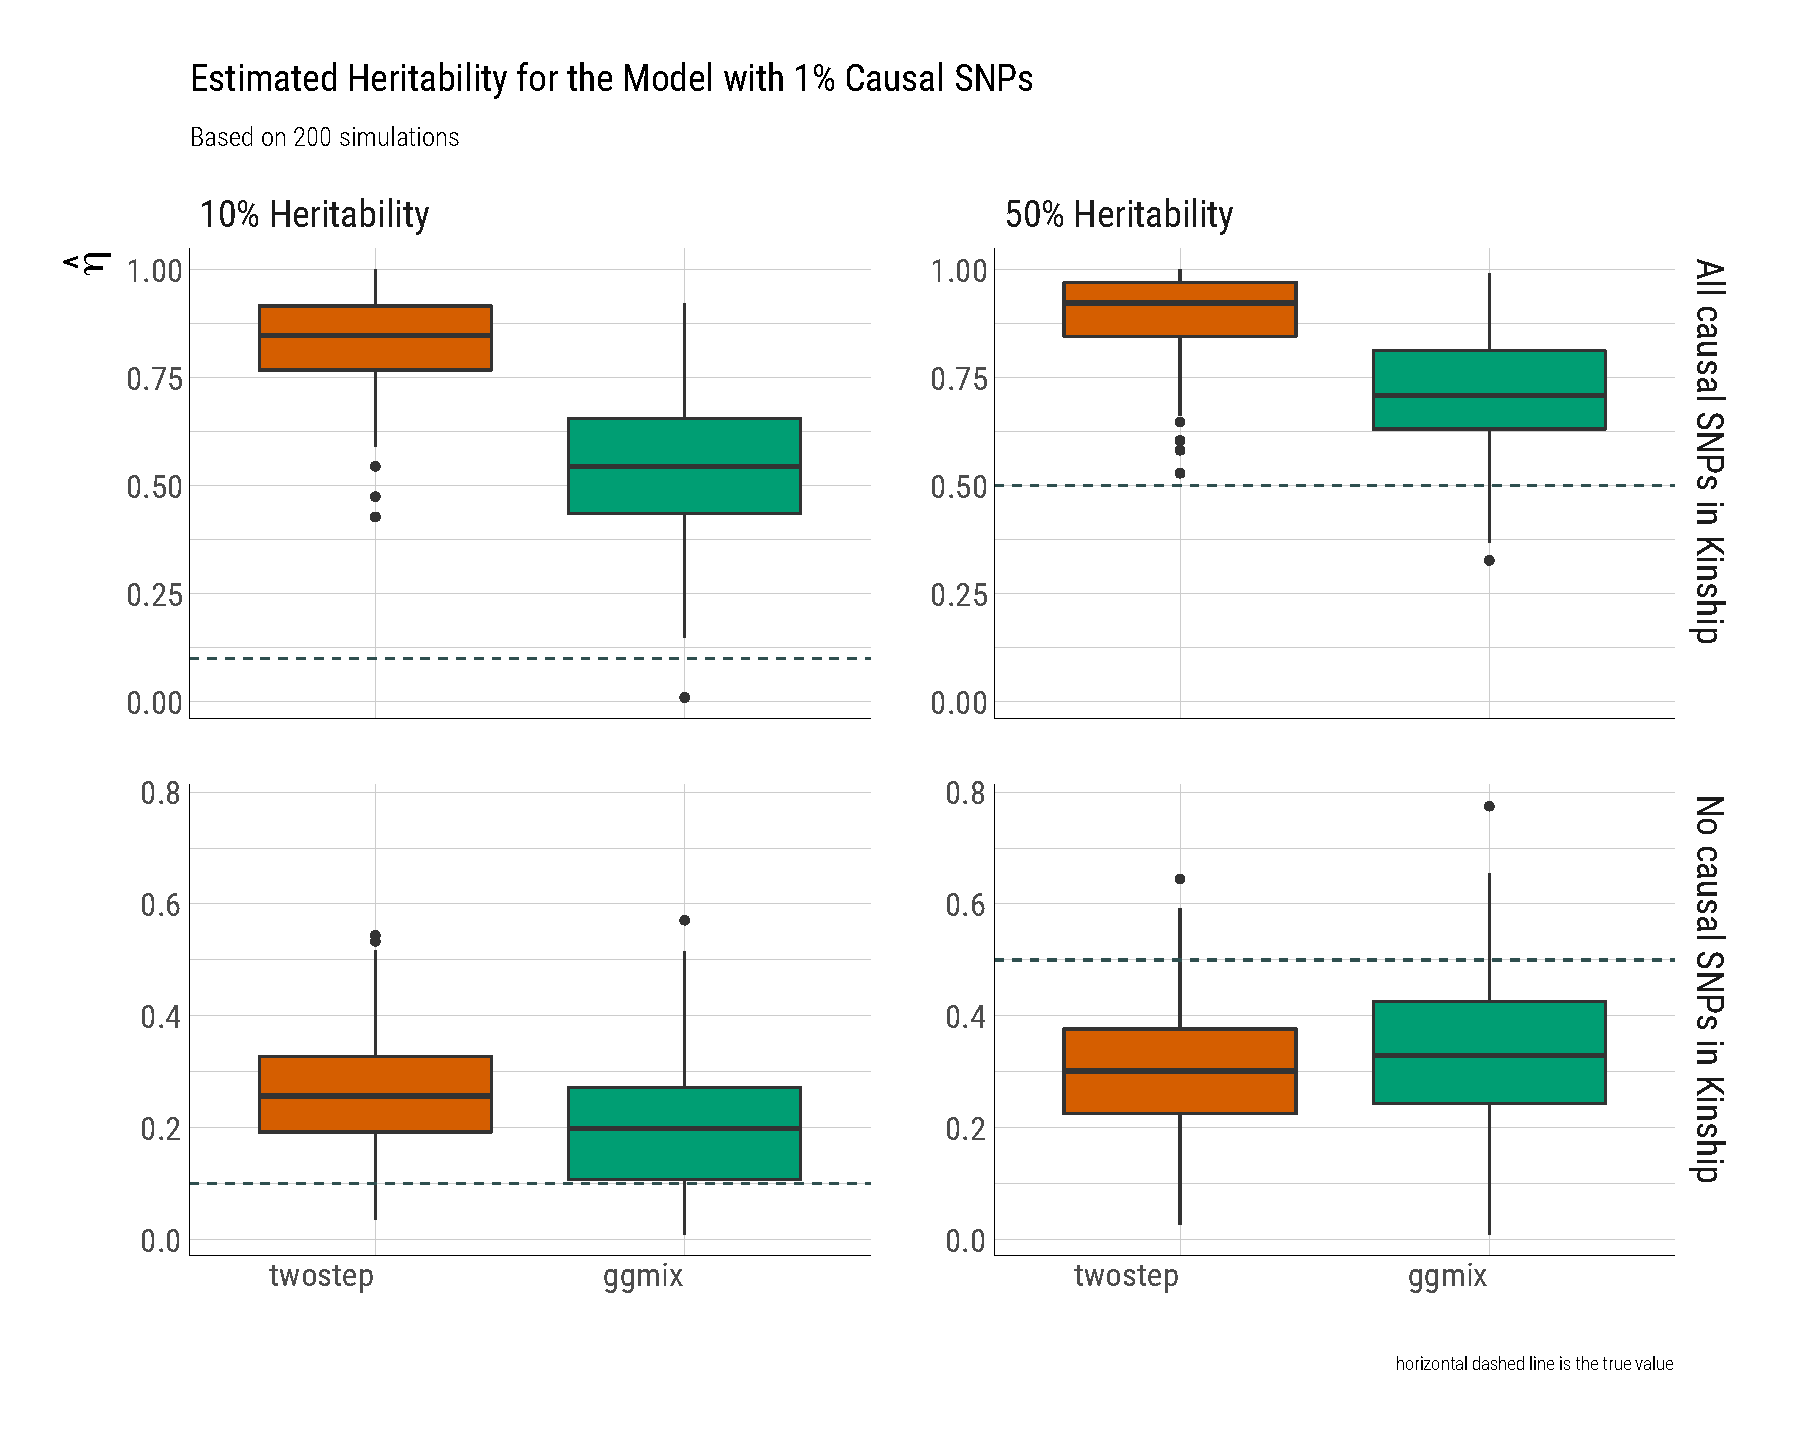
\includegraphics[width=1\linewidth]{figure/plot-eta-sim-1p-causal-1} 

}

\caption[Boxplot of $\hat{\eta}$ in the \texttt{ggmix} model from 200 simulations by kinship geography and number of causal SNPs that were included in the calculation of the kinship matrix]{Boxplot of $\hat{\eta}$ in the \texttt{ggmix} model from 200 simulations by kinship geography and number of causal SNPs that were included in the calculation of the kinship matrix.}\label{fig:plot-eta-sim-1p-causal}
\end{figure}


\end{knitrout}


\begin{knitrout}\scriptsize
\definecolor{shadecolor}{rgb}{0.969, 0.969, 0.969}\color{fgcolor}\begin{figure}[H]

{\centering 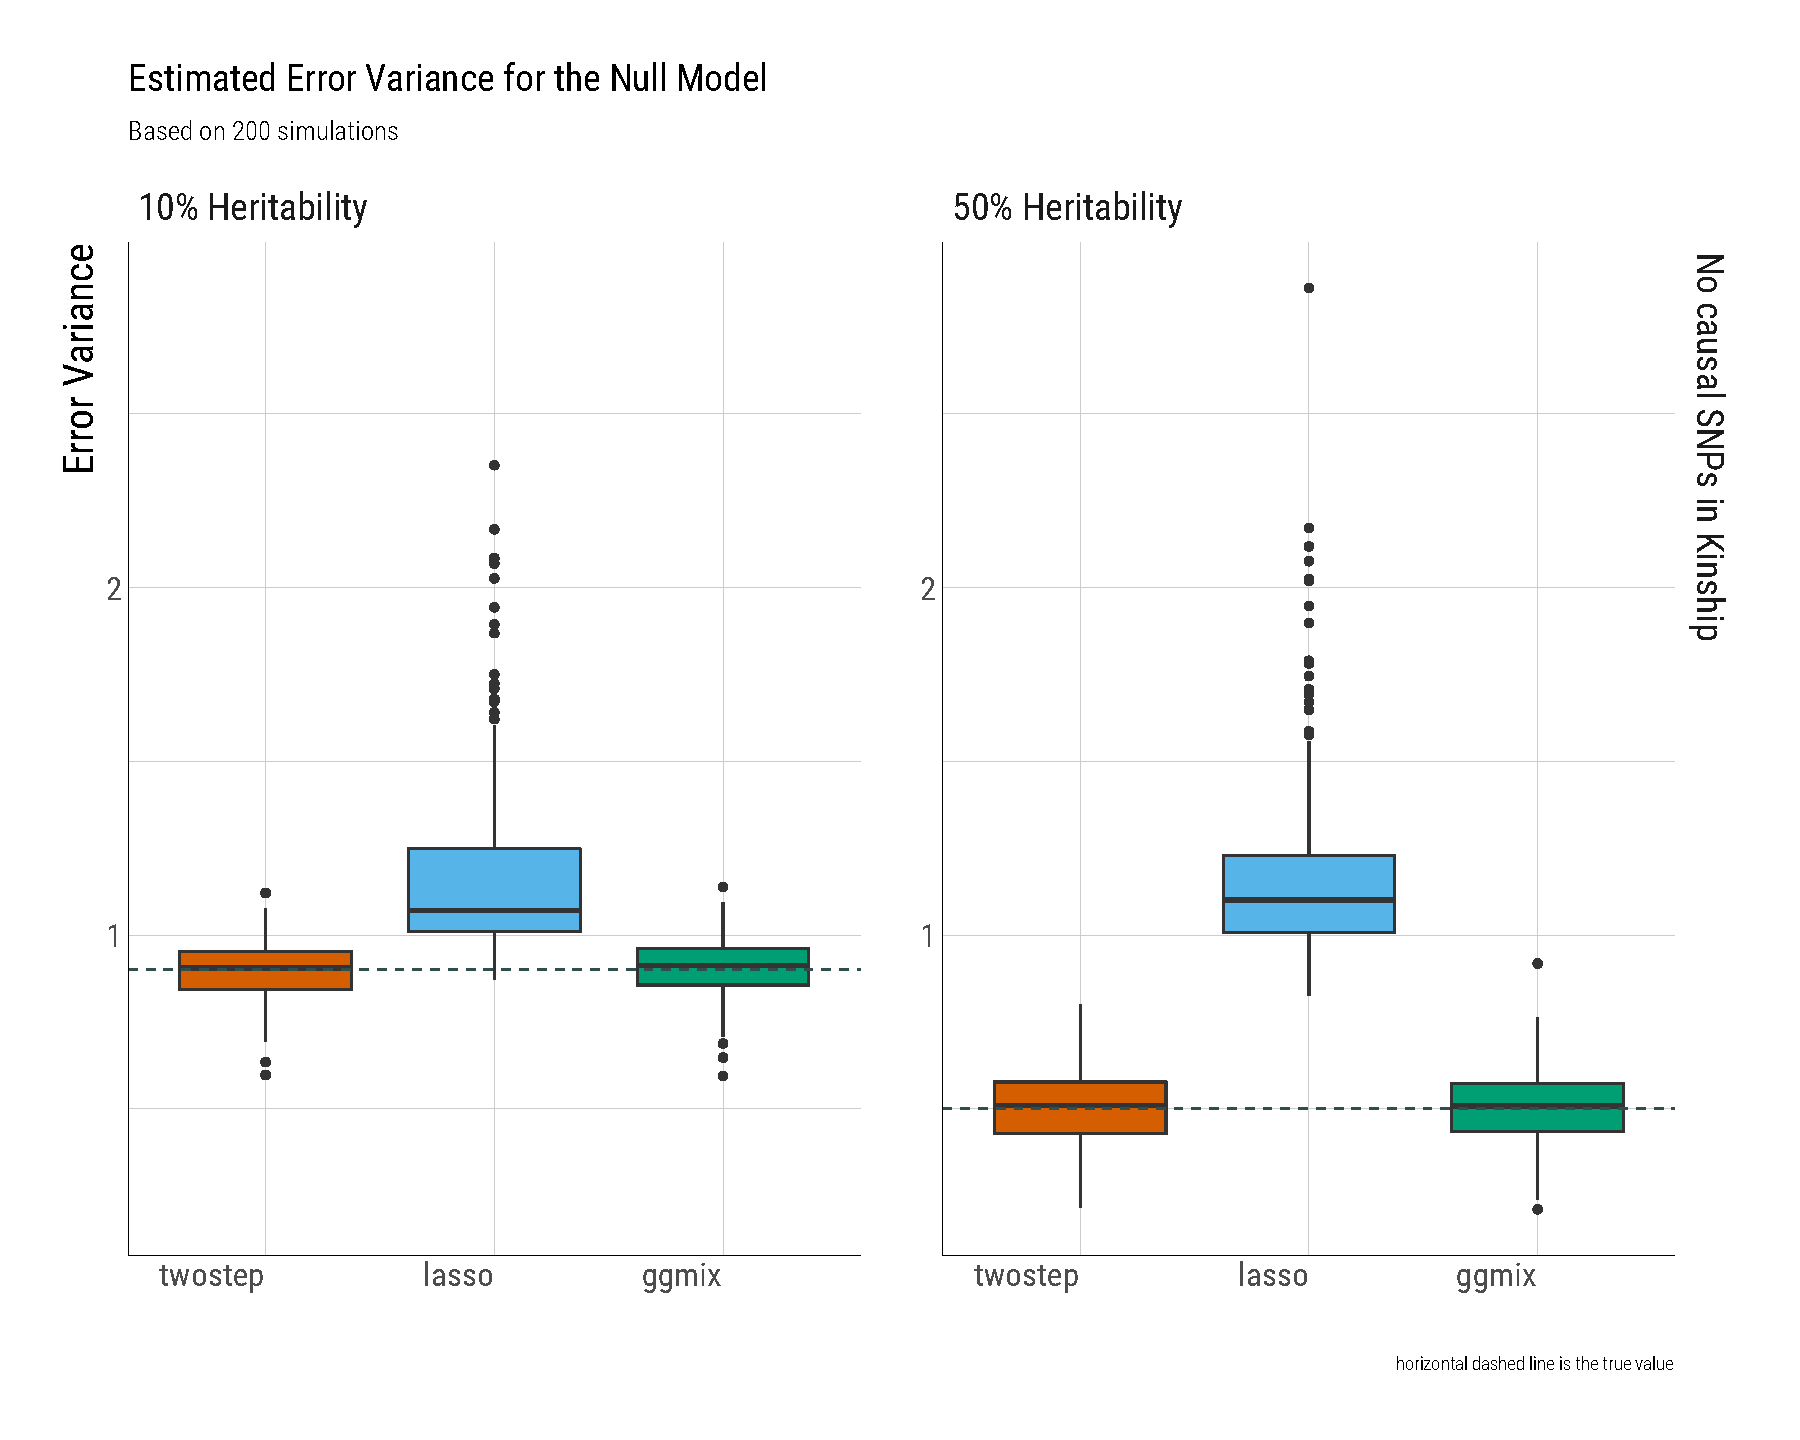
\includegraphics[width=1\linewidth]{figure/plot-errorvar-sim-null-model-1} 

}

\caption[Means $\pm 1$ standard deviation of error variance from 200 simulations by kinship geography and number of causal SNPs that were included in the calculation of the kinship matrix]{Means $\pm 1$ standard deviation of error variance from 200 simulations by kinship geography and number of causal SNPs that were included in the calculation of the kinship matrix.}\label{fig:plot-errorvar-sim-null-model}
\end{figure}


\end{knitrout}

\begin{knitrout}\scriptsize
\definecolor{shadecolor}{rgb}{0.969, 0.969, 0.969}\color{fgcolor}\begin{figure}[H]

{\centering 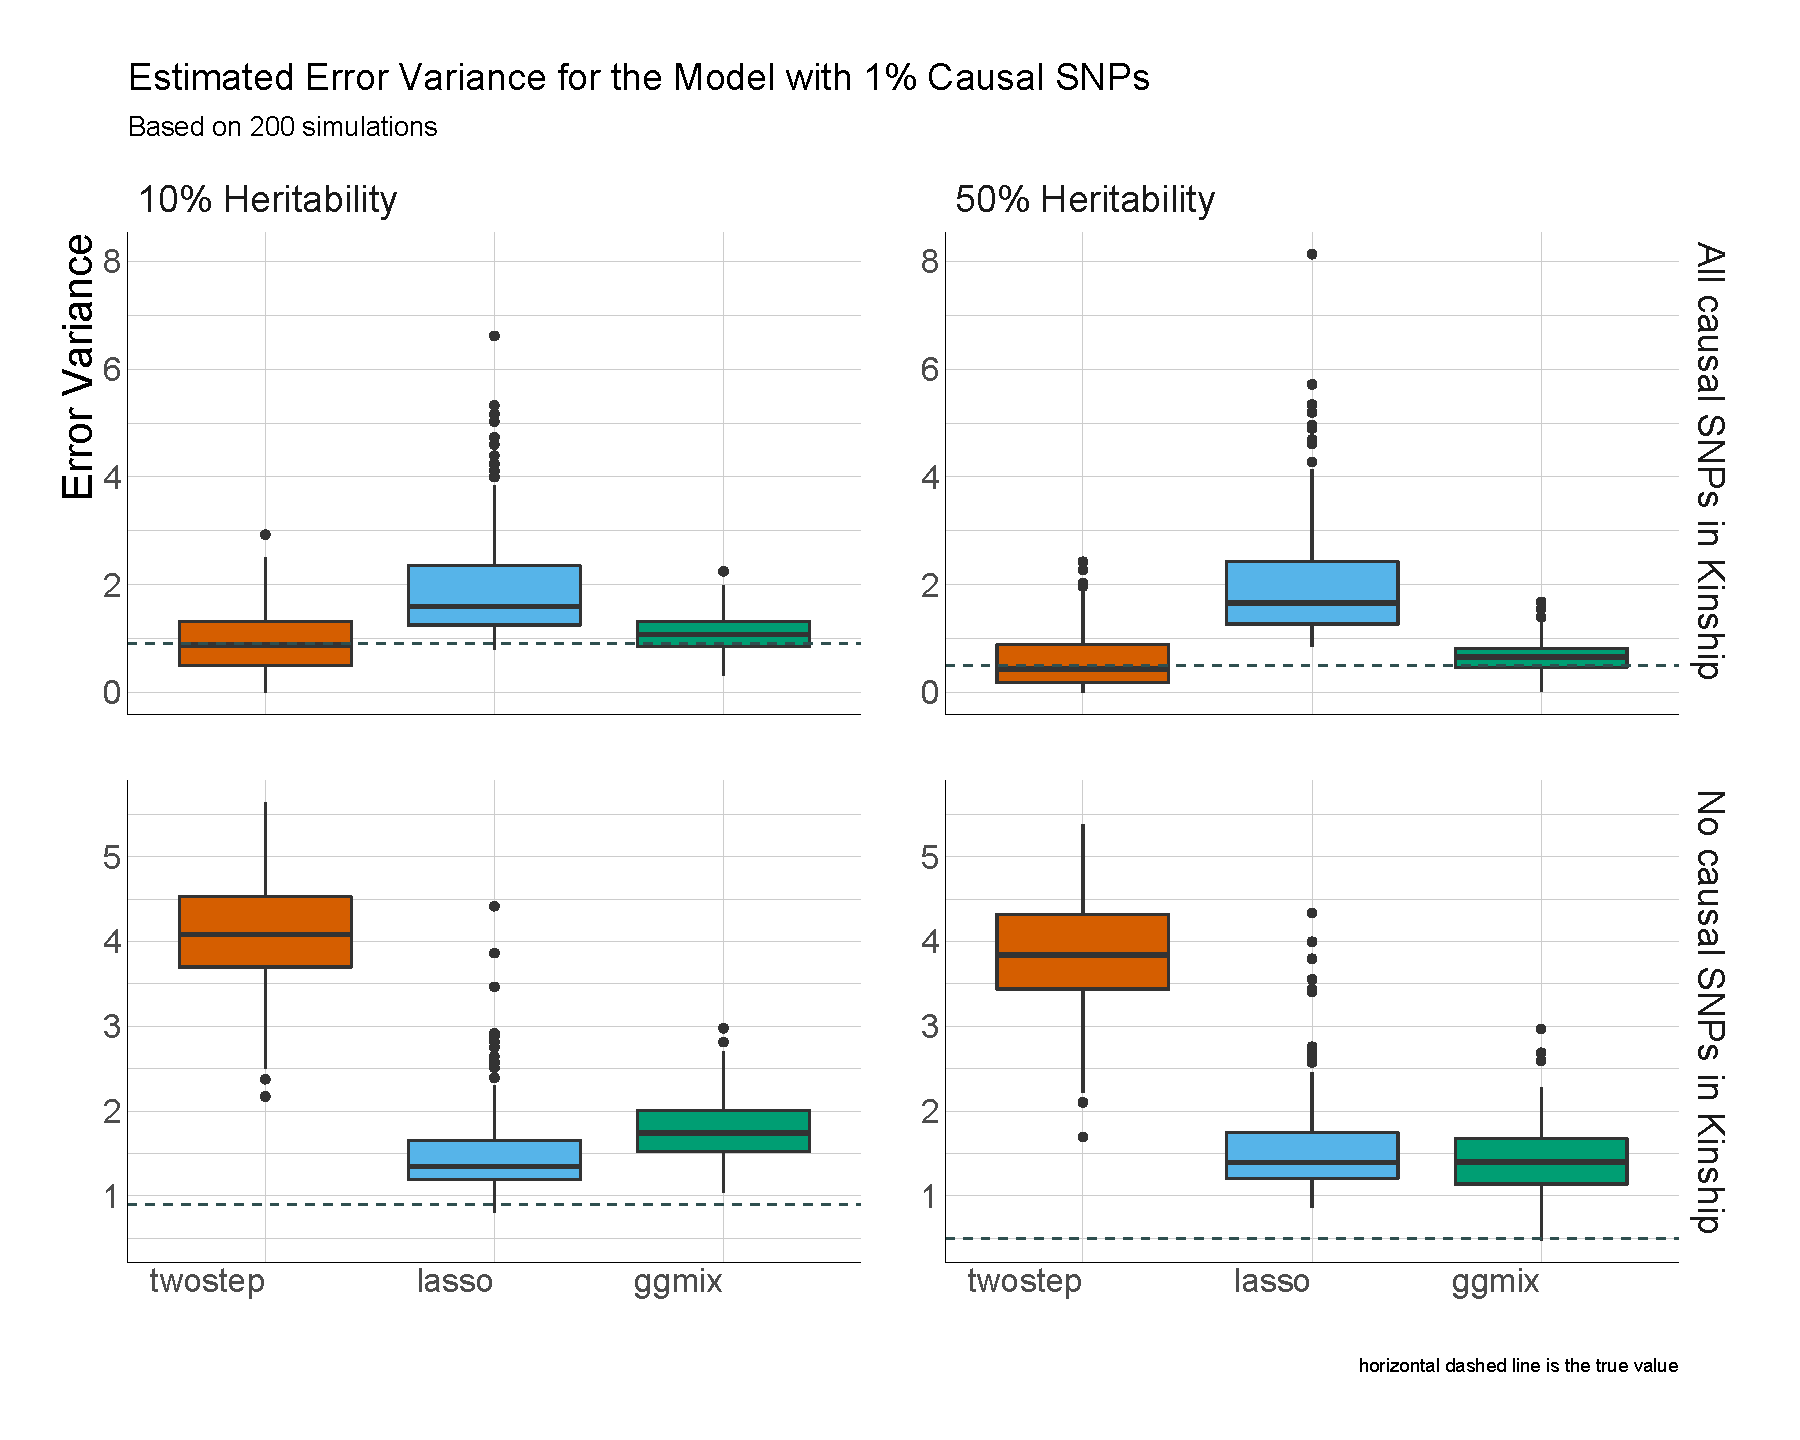
\includegraphics[width=1\linewidth]{figure/plot-errorvar-sim-1p-causal-1} 

}

\caption[Means $\pm 1$ standard deviation of error variance from 200 simulations by kinship geography and number of causal SNPs that were included in the calculation of the kinship matrix]{Means $\pm 1$ standard deviation of error variance from 200 simulations by kinship geography and number of causal SNPs that were included in the calculation of the kinship matrix.}\label{fig:plot-errorvar-sim-1p-causal}
\end{figure}


\end{knitrout}



\begin{knitrout}\scriptsize
\definecolor{shadecolor}{rgb}{0.969, 0.969, 0.969}\color{fgcolor}\begin{figure}[H]

{\centering 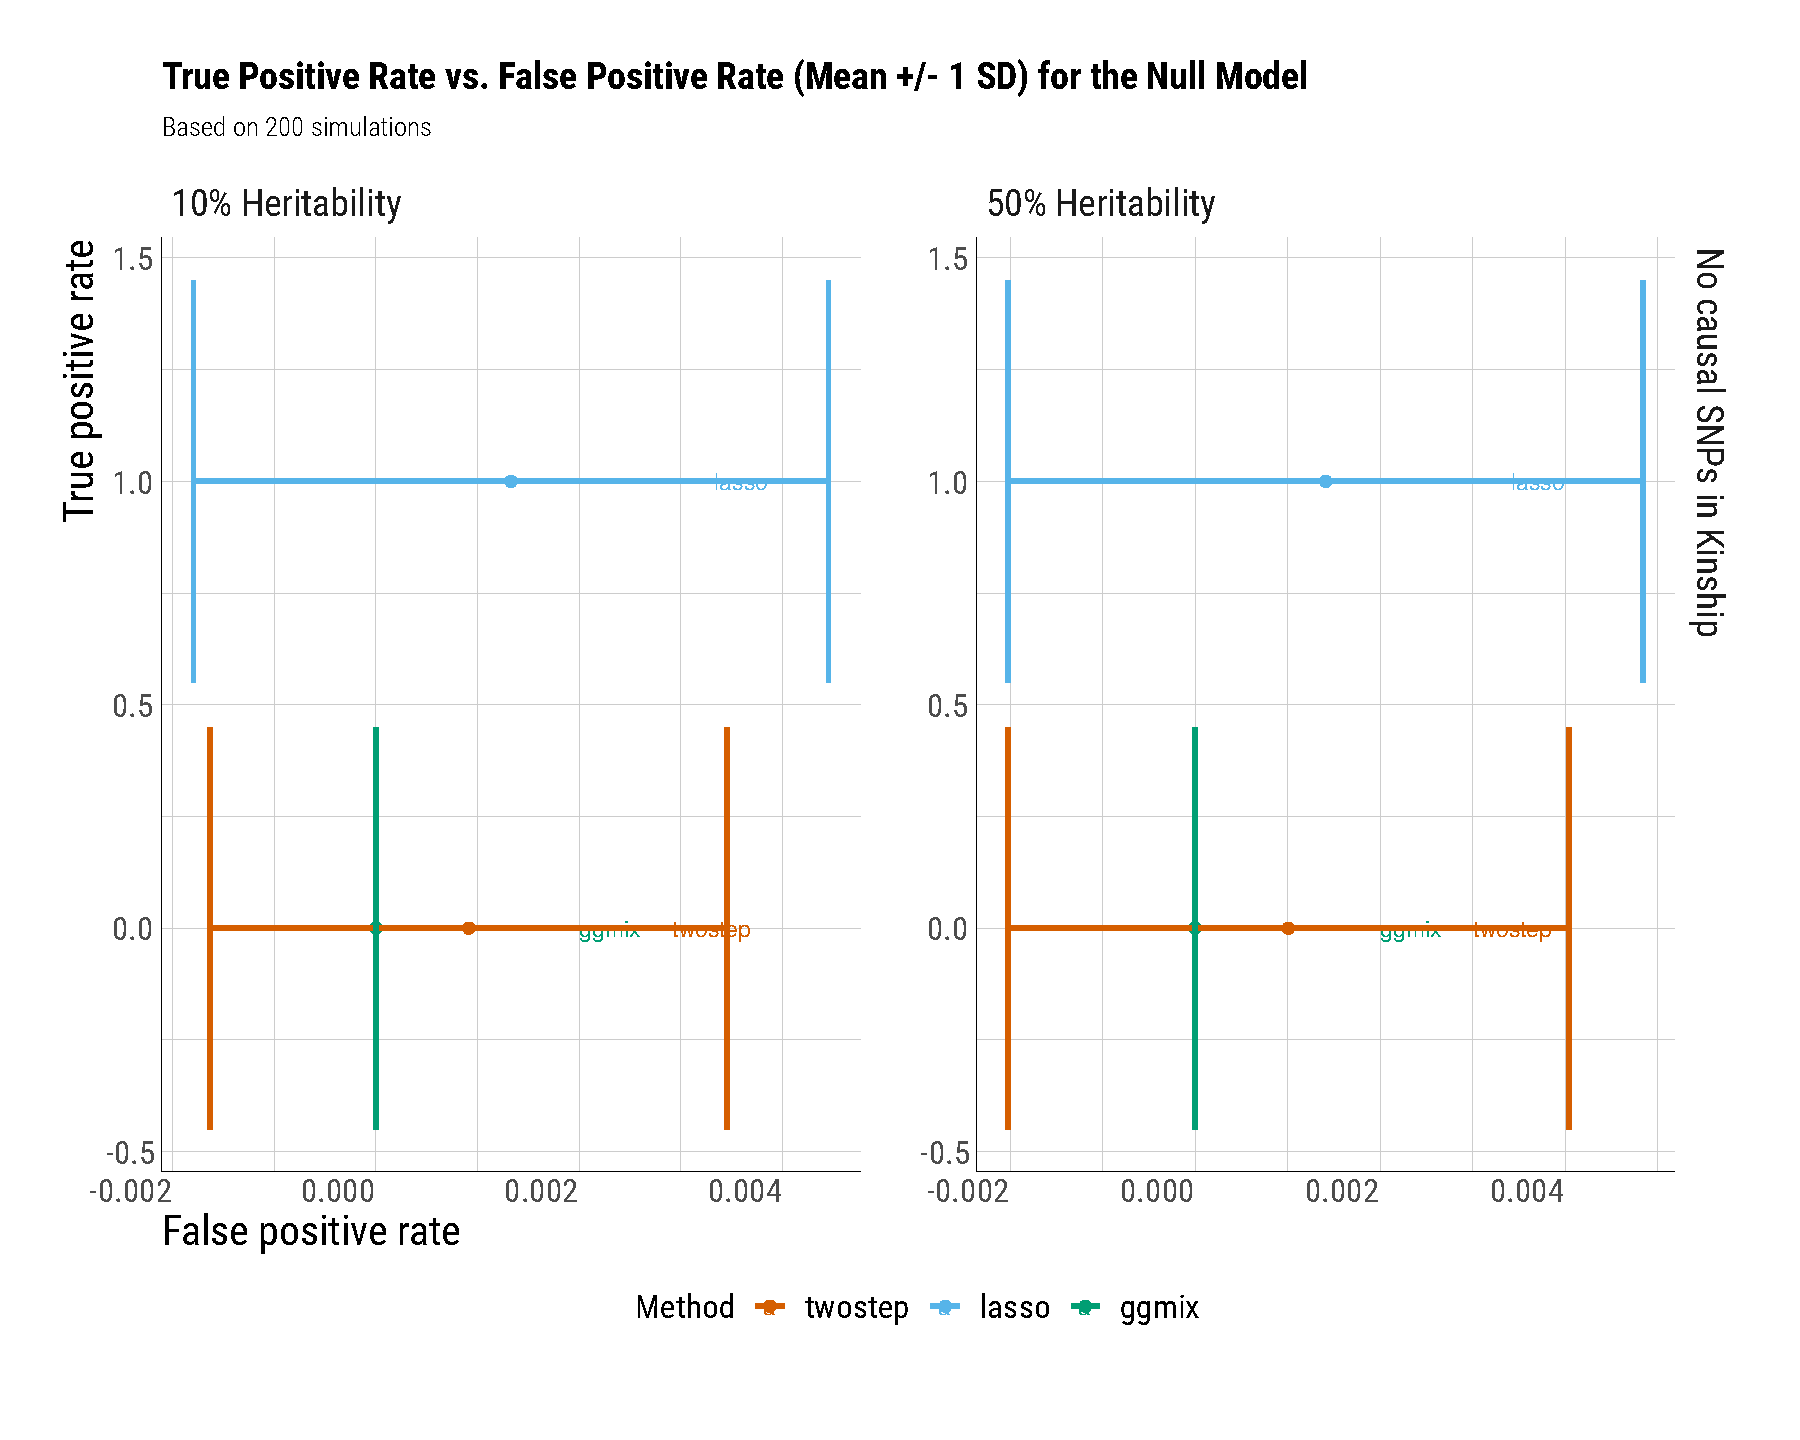
\includegraphics[width=1\linewidth]{figure/plot-tpr-fpr-sim-null-model-1} 

}

\caption[Means $\pm 1$ standard deviation of true positive rate vs]{Means $\pm 1$ standard deviation of true positive rate vs. false positive rate from 200 simulations by kinship geography and number of causal SNPs that were included in the calculation of the kinship matrix.}\label{fig:plot-tpr-fpr-sim-null-model}
\end{figure}


\end{knitrout}

\begin{knitrout}\scriptsize
\definecolor{shadecolor}{rgb}{0.969, 0.969, 0.969}\color{fgcolor}\begin{figure}[H]

{\centering 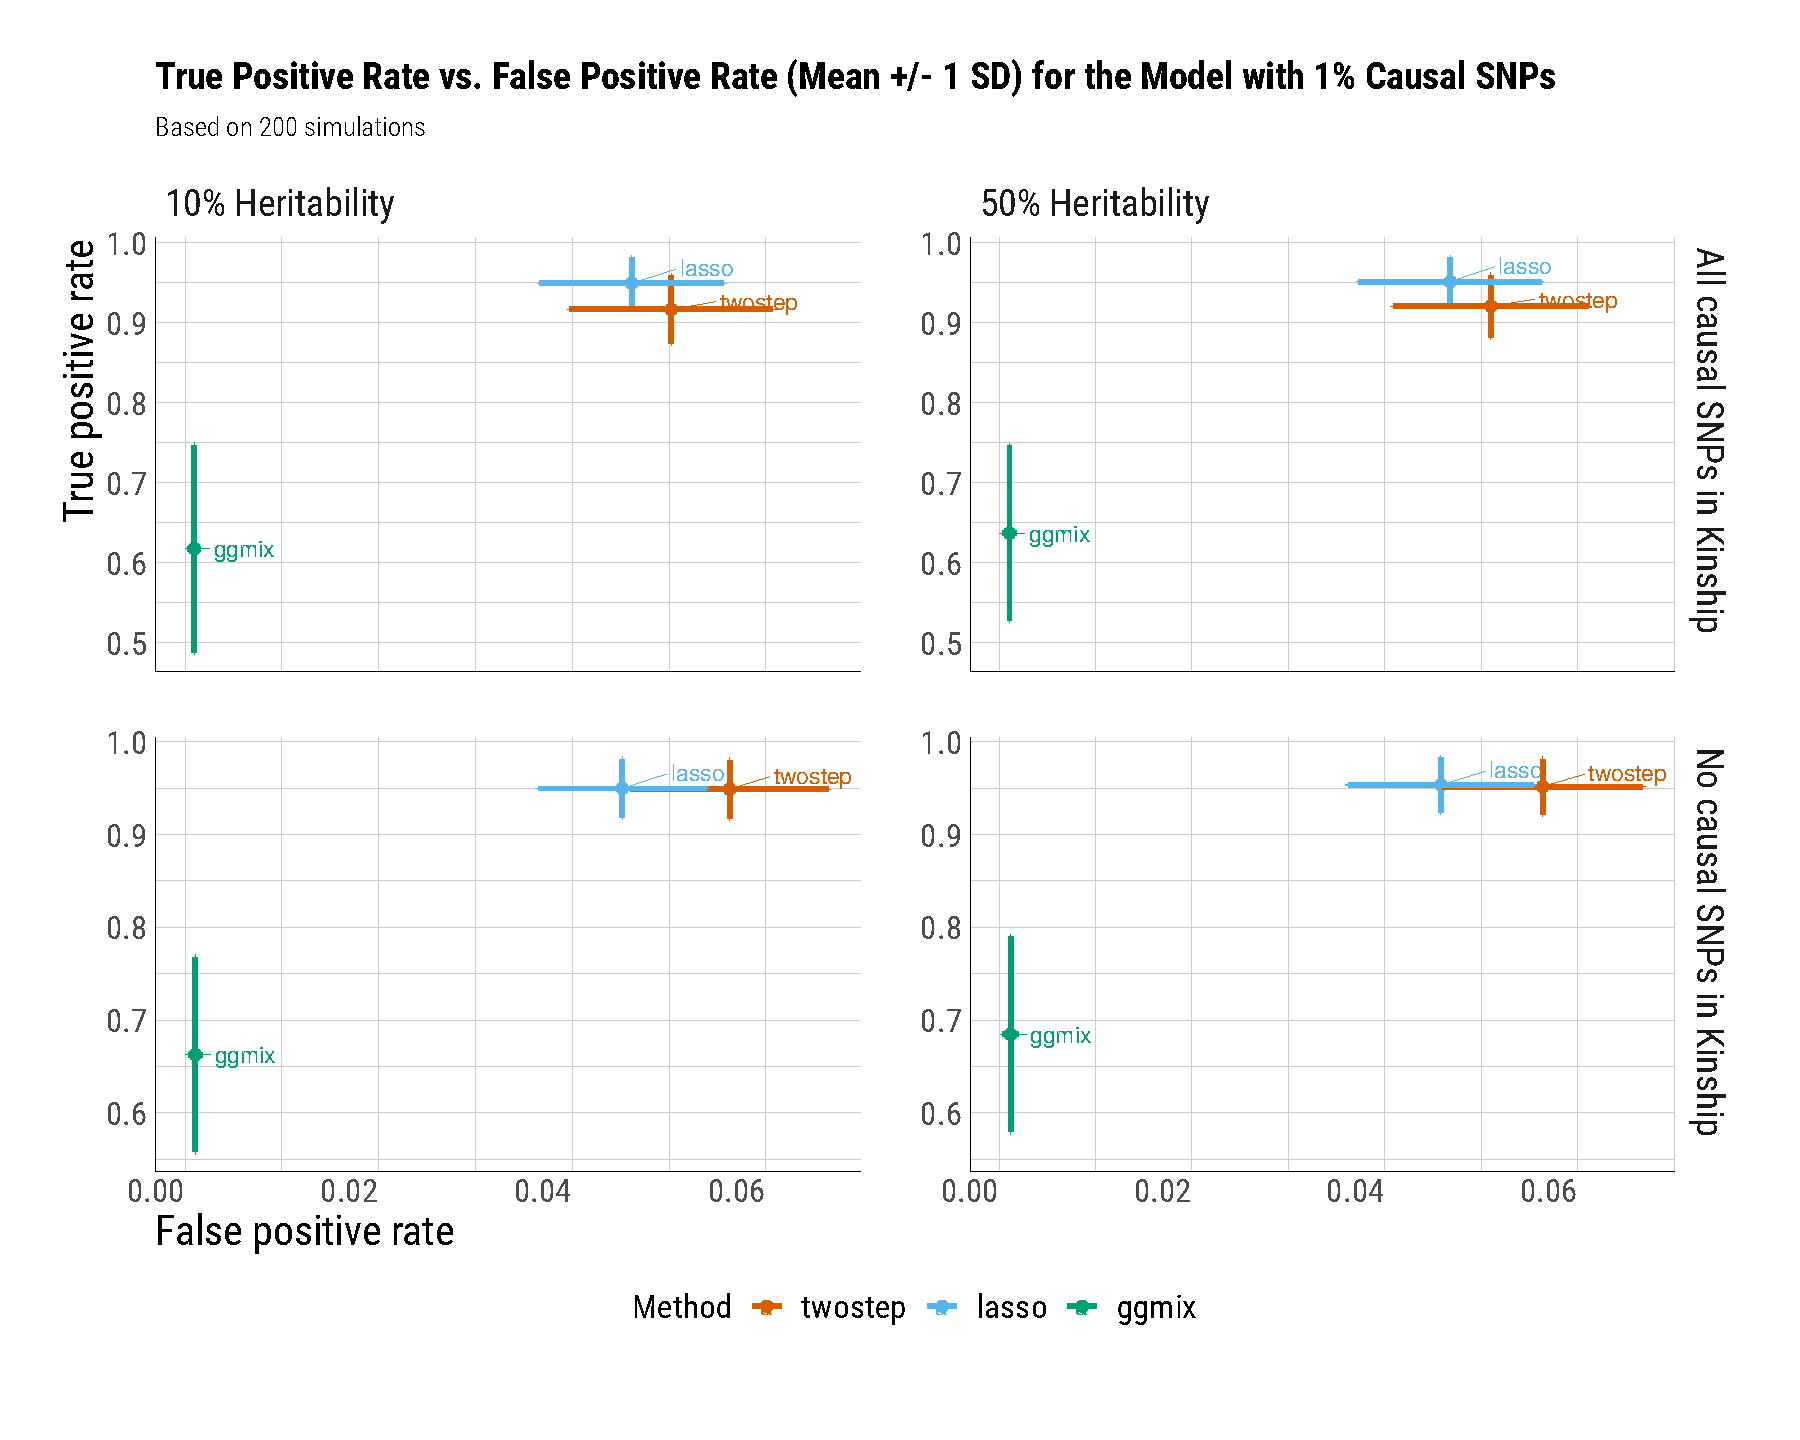
\includegraphics[width=1\linewidth]{figure/plot-tpr-fpr-sim-1p-causal-1} 

}

\caption[Means $\pm 1$ standard deviation of true positive rate vs]{Means $\pm 1$ standard deviation of true positive rate vs. false positive rate from 200 simulations by kinship geography and number of causal SNPs that were included in the calculation of the kinship matrix.}\label{fig:plot-tpr-fpr-sim-1p-causal}
\end{figure}


\end{knitrout}





\section{Discussion}

We develop a general penalized LMM framework that simultaneously selects and estimates variables, accounting for between individual correlations, in one step. Our method can accommodate several sparsity inducing penalties such as the lasso, elastic net and group lasso, and also readily handles prior annotation information in the form of weights. We develop a groupwise-majorization descent algorithm which is highly scalable, computationally efficient and has theoretical guarantees of the convergence. Through simulations, we show that are method has better power over the two-stage approach, particularly for polygenic traits.

While the predominant motivation for these methods has been association testing, we believe that there are other applications in which they can be used as well. 
For example, in the most recent Genetic Analysis Workship 20 (GAW20),  the causal modeling group investigated causal
relationships between DNA methylation (exposure) within some genes
and the change in high-density lipoproteins $\Delta$HDL (outcome) using Mendelian randomization (MR)~\citep{davey2003mendelian}. 
Penalized regression methods could be used to select SNPs strongly associated with the exposure in order to be used as an instrumental variable (IV). 
However, since GAW20 data consisted of families, two step methods were used which could have resulted in a loss of power. \ggmix~is an alternative approach that could be used for selecting the IV while accounting for the familial structure of the data. 
Our method is also suitable for fine mapping SNP association signals in genomic regions, where the goal is to pinpoint individual variants most likely to impact the undelying biological mechanisms of disease~\citep{spain2015strategies}.

\begin{comment}
\subsection{Real Data UKBiobank}

Use height as a phenotype as it is known to be related to lots of SNPs with small effects (see paper by Peter Visher, Nature Genetics 2010).


Use 301 SNPs plus those that are in LD. Make sure that overlap is strong with the 300.



\subsection{Extension to Elastic Net}


\subsection{Is there a way to show mathematically, situations where two step is worse than one step?}

\subsection{Other Details}

Since we include a column of ones in our design matrix $\bX$, the first column of the rotation $\bXtilde = \bU^T\bX$ corresponds to the intercept. Therefore, when using \texttt{glmnet} to update $\bbeta$ in Algorithm~\ref{alg:cgd2}, we specify \texttt{intercept = FALSE} and a \texttt{penalty.factor = c(0, rep(1, p))} so that the intercept does not get penalized. Furthermore we specify \texttt{standardize = FALSE}.
\end{comment}










\begin{comment}
\section{General Notes}

\begin{itemize}
\item One way in which spurious associations occur in the presence of
population structure is that SNPs become correlated with each other
when structure is not taken into account~\citep{song2015testing}
\item  For the remainder of the manuscript we therefore focus
on results obtained using the pruned set of SNPs to estimate
kinships (apart for genome-wide analysis in the program Mendel,
which by default always uses the entire set of SNPs that has been
read in)~\citep{eu2014comparison}
\item Most LMM packages (although not Mendel) allow a separation
between the 'estimation of kinships' step and the 'association
testing' step. This is convenient as it allows the user to read in
theoretical or estimated kinships as desired, and to consider using
an alternative package for estimating kinships to the one used for
the actual association testing~\citep{eu2014comparison}
\item Since many groups (including ourselves)
use PLINK [27] to perform initial quality control of genome-wide
association data, we considered programs that could use PLINK
files directly (or with just a few easily-implemented transformation
steps) to be the easiest to use, while those programs that required
more extensive data transformation, creation of additional input
files and/or external estimation of kinships were considered
harder~\citep{eu2014comparison}
\item  investigated a strategy for
analysing longitudinal traits (repeated measures) in a linear mixed
model framework simply by treating each measurement as if it
came from a different individual, and expanding out the genetic
data set accordingly (resulting in an expanded data set containing
many apparent twins, triplets, quadruplets etc., depending on how
many measurements are available for each person).~\citep{eu2014comparison}
\end{itemize}
\end{comment}






\newpage


%\bibliographystyle{unsrt}
%\bibliography{GEbib}

\bibliographystyle{unsrt}
\bibliography{ggmixbib}

\newpage

\appendix
%\counterwithin{figure}{section}

\section{Block Coordinate Descent Algorithm} \label{ap:cgd}

We use a general purpose block coordinate descent algorithm (CGD)~\citep{tseng2009coordinate} to solve~\eqref{eq:estimator}. At each iteration, the algorithm approximates the negative log-likelihood $f(\cdot)$ in $Q_{\lambda}(\cdot)$ by a strictly convex quadratic function and then applies block coordinate decent to generate a decent direction followed by an inexact line search along this direction~\citep{tseng2009coordinate}. For continuously differentiable $f(\cdot)$ and convex and block-separable $P(\cdot)$ \mbox{(i.e. $P(\bbeta) = \sum_i P_i (\beta_i)$)},~\cite{tseng2009coordinate} show that the solution generated by the CGD method is a stationary point of $Q_{\lambda}(\cdot)$ if the coordinates are updated in a Gauss-Seidel manner i.e. $Q_{\lambda}(\cdot)$ is minimized with respect to one parameter while holding all others fixed. The CGD algorithm can thus be run in parallel and therefore suited for large $p$ settings. It has been successfully applied in fixed effects models (e.g.~\cite{meier2008group},~\cite{friedman2010regularization}) and~\cite{schelldorfer2011estimation} for mixed models with an $\ell_1$ penalty. Following Tseng and Yun~\cite{tseng2009coordinate}, the CGD algorithm is given by Algorithm~\ref{alg:cgd}.

\begin{algorithm}[htbp]
	\SetAlgoLined
	%	\KwResult{Write here the result }
	Set the iteration counter $k \leftarrow 0$ and choose initial values for the parameter vector $\bTheta^{(0)}$\;
	\Repeat{convergence criterion is satisfied}{
		Approximate the Hessian $\nabla^2 f(\bTheta^{(k)})$ by a symmetric matix $H^{(k)}$:
		\begin{equation}
			H^{(k)} = \diag \left[ \min \left\lbrace \max \left\lbrace \left[ \nabla^2 f(\bTheta^{(k)})\right] _{jj}, c_{min} \right\rbrace c_{max} \right\rbrace\right]_{j = 1, \ldots, p+1} \label{eq:Hk}
		\end{equation}
		\For{$ j =1, \ldots, p+1$}{
			
			Solve the descent direction $d^{(k)} \coloneqq d_{H^{(k)}}(\Theta_{j}^{(k)})$ \;
			
			\If{$\Theta_j^{(k)} \in \left\lbrace \beta_1, \ldots, \beta_p \right\rbrace$}{
				\begin{equation}
					d_{H^{(k)}}(\Theta_{j}^{(k)}) \leftarrow \argmin_{d} \left\lbrace \nabla f(\Theta_{j}^{(k)}) d + \frac{1}{2} d^2 H^{(k)}_{j j} + \lambda P(\Theta_{j}^{(k)} + d) \right\rbrace \label{eq:descentdirection}
				\end{equation}
			}{ \If{$\Theta_j^{(k)} \in \left\lbrace \eta \right\rbrace$}{
				\begin{equation}
					d_{H^{(k)}}(\Theta_{j}^{(k)}) \leftarrow - \nabla f(\Theta_{j}^{(k)}) / H_{jj}^{(k)}
				\end{equation}
			}{
			
			
		}
	}
	Choose a stepsize\;
	\begin{equation*}
		\alpha_j^{(k)} \leftarrow \tm{line search given by the Armijo rule}
	\end{equation*}
	Update\;
	\begin{equation*}
		\widehat{\Theta}_j^{(k+1)} \leftarrow \widehat{\Theta}_j^{(k)} + \alpha_j^{(k)}d^{(k)}
	\end{equation*}
}
Update\;
\begin{equation}
	\widehat\eta^{(k+1)} \leftarrow \argmin_{\eta}  \frac{1}{2} \sum_{i=1}^{N_T} \log(1 + \eta (\Lambda_i-1)) + \frac{1}{2{\sigma^2}^{\,(k)}} \sum_{i=1}^{N_T}\frac{\left(  \Ytilde_i - \sum_{j=0}^{p}\Xtilde_{ij+1}\beta_j^{(k+1)} \right) ^2}{1 + \eta (\Lambda_i-1)}
\end{equation}
Update\;
\begin{equation}
	%\widehat{\sigma^2}^{\,\,(k+1)} \leftarrow \frac{1}{N_T}\sum_{i=1}^{N_T}\frac{([ \bYtilde - \bXtilde \widehat{\bbeta}^{(k+1)}]_i )^2}{1 + \widehat{\eta}^{(k+1)} (\Lambda_i-1)}
	\widehat{\sigma^2}^{\,\,(k+1)} \gets \frac{1}{N_T}\sum_{i=1}^{N_T}\frac{\left(  \Ytilde_i - \sum_{j=0}^{p}\Xtilde_{ij+1}\beta_j^{(k+1)} \right) ^2}{1 + \eta^{(k+1)} (\Lambda_i-1)}
\end{equation}
$k \leftarrow k +1$
}
\caption{Coordinate Gradient Descent Algorithm to solve~\eqref{eq:estimator}} \label{alg:cgd}
\end{algorithm}

\begin{comment}
We note that conditional on $\widehat{\bbeta}$ and $\widehat{\eta}$, there exists an analytic solution for $\widehat{\sigma^2}$:
\begin{align}
	\frac{\partial}{\partial \sigma^2} f(\bTheta) &= \frac{N_T}{2\sigma^2}- \frac{1}{2\sigma^4} \sum_{i=1}^{N_T}\frac{([ \bYtilde - \bXtilde \bbeta]_i )^2}{1 + \eta (\Lambda_i-1)} = 0 \nonumber \\
	\widehat{\sigma^2} & = \frac{1}{N_T}\sum_{i=1}^{N_T}\frac{([ \bYtilde - \bXtilde \widehat{\bbeta}]_i )^2}{1 + \widehat{\eta} (\Lambda_i-1)} \label{eq:sigmahat}
\end{align}
\end{comment}

The Armijo rule is defined as follows~\citep{tseng2009coordinate}:
\begin{tcolorbox}
	Choose $\alpha_{init}^{(k)}>0$ and let $\alpha^{(k)}$ be the largest element of $\left\lbrace \alpha_{init}^k \delta^r \right\rbrace_{r = 0,1,2,\ldots} $ satisfying
	\begin{equation}
		Q_{\lambda}(\Theta_j^{(k)} + \alpha^{(k)} d^{(k)}) \leq Q_{\lambda} (\Theta_j^{(k)}) + \alpha^{(k)}\varrho \Delta^{(k)}
	\end{equation}
	where $0 < \delta <1$, $0 < \varrho <1$, $0 \leq \gamma < 1$ and
	\begin{equation}
		\Delta^{(k)} \coloneqq \nabla f(\Theta_j^{(k)})d^{(k)} + \gamma (d^{(k)})^2 H^{(k)}_{jj} + \lambda P(\Theta_j^{(k)} + d^{(k)}) - \lambda P(\Theta^{(k)})
	\end{equation}
\end{tcolorbox}
Common choices for the constants are $\delta=0.1$, $\varrho=0.001$, $\gamma = 0$, $\alpha_{init}^{(k)} = 1$ for all $k$~\citep{schelldorfer2011estimation}.

Below we detail the specifics of Algorithm~\ref{alg:cgd} for the $\ell_1$ penalty.

\subsection{$\ell_1$ penalty}\label{subsec:l1penalty}

The objective function is given by
\begin{equation}
	Q_{\lambda}(\bTheta) = f(\bTheta) + \lambda |\bbeta|
\end{equation}


\subsubsection{Descent Direction}
For simplicity, we remove the iteration counter $(k)$ from the derivation below.\\ For \mbox{$\Theta_j^{(k)} \in \left\lbrace \beta_1, \ldots, \beta_p \right\rbrace$}, let
\begin{equation}
	d_{H}(\Theta_{j}) = \argmin_{d} G(d)  \label{eq:argminGd}
\end{equation}
where
\[ G(d) =  \nabla f(\Theta_{j}) d + \frac{1}{2} d^2 H_{j j} + \lambda |\Theta_{j} + d| \]
Since $G(d)$ is not differentiable at $-\Theta_j$, we calculate the subdifferential $\partial G(d)$ and search for $d$ with $0 \in \partial G(d)$:
\begin{equation}
	\partial G(d) = \nabla f(\Theta_{j}) + d H_{j j} + \lambda u   \label{eq:subdiff}
\end{equation}
where
\begin{equation}
	u = \begin{cases}
		1 & \tm{if\quad}d > -\Theta_j \\
		-1 & \tm{if\quad} d < -\Theta_j\\
		[-1,1] & \tm{if\quad} d = \Theta_j
	\end{cases}
\end{equation}
We consider each of the three cases in~\eqref{eq:subdiff} below
\begin{enumerate}
	\item $d > -\Theta_j$
	\begin{align}
		\partial G(d) & = \nabla f(\Theta_{j}) + d H_{j j} + \lambda = 0 \nonumber \\
		d & = \frac{-(\nabla f(\Theta_{j}) + \lambda)}{H_{j j}}  \nonumber
	\end{align}
	Since $\lambda>0$ and $H_{jj}>0$, we have
	\begin{equation*}
		\frac{-(\nabla f(\Theta_{j}) - \lambda)}{H_{j j}} > \frac{-(\nabla f(\Theta_{j}) + \lambda)}{H_{j j}} = d \overset{\tm{def}}{>} -\Theta_j
	\end{equation*}
	The solution can be written compactly as
	\begin{equation*}
		d = \tm{mid}\left\lbrace \frac{-(\nabla f(\Theta_{j}) - \lambda)}{H_{j j}}, -\Theta_j ,\frac{-(\nabla f(\Theta_{j}) + \lambda)}{H_{j j}} \right\rbrace
	\end{equation*}
	where $\tm{mid}\left\lbrace a,b,c \right\rbrace$ denotes the median (mid-point) of $a,b,c$~\citep{tseng2009coordinate}.
	\item $d < -\Theta_j$
	\begin{align}
		\partial G(d) & = \nabla f(\Theta_{j}) + d H_{j j} - \lambda = 0 \nonumber \\
		d & = \frac{-(\nabla f(\Theta_{j}) - \lambda)}{H_{j j}}  \nonumber
	\end{align}
	Since $\lambda>0$ and $H_{jj}>0$, we have
	\begin{equation*}
		\frac{-(\nabla f(\Theta_{j}) + \lambda)}{H_{j j}} < \frac{-(\nabla f(\Theta_{j}) - \lambda)}{H_{j j}} = d \overset{\tm{def}}{<} -\Theta_j
	\end{equation*}
	Again, the solution can be written compactly as
	\begin{equation*}
		d = \tm{mid}\left\lbrace \frac{-(\nabla f(\Theta_{j}) - \lambda)}{H_{j j}}, -\Theta_j ,\frac{-(\nabla f(\Theta_{j}) + \lambda)}{H_{j j}} \right\rbrace
	\end{equation*}
	
	\item $d_j = -\Theta_j$\\
	There exists $u \in [-1,1]$ such that
	\begin{align*}
		\partial G(d) & = \nabla f(\Theta_{j}) + d H_{j j} + \lambda u = 0 \nonumber \\
		d & = \frac{-(\nabla f(\Theta_{j}) + \lambda u)}{H_{j j}}  \nonumber
	\end{align*}
	For $-1 \leq u \leq 1$, $\lambda>0$ and $H_{jj}>0$ we have
	\begin{equation*}
		\frac{-(\nabla f(\Theta_{j}) + \lambda)}{H_{j j}} \leq  d \overset{\tm{def}}{=} -\Theta_j \leq \frac{-(\nabla f(\Theta_{j}) - \lambda)}{H_{j j}}
	\end{equation*}
	The solution can again be written compactly as
	\begin{equation*}
		d = \tm{mid}\left\lbrace \frac{-(\nabla f(\Theta_{j}) - \lambda)}{H_{j j}}, -\Theta_j ,\frac{-(\nabla f(\Theta_{j}) + \lambda)}{H_{j j}} \right\rbrace
	\end{equation*}
	
\end{enumerate}
We see all three cases lead to the same solution for~\eqref{eq:argminGd}. Therefore the descent direction for $\Theta_j^{(k)} \in \left\lbrace \beta_1, \ldots, \beta_p \right\rbrace$ for the $\ell_1$ penalty is given by
\begin{equation}
	d = \tm{mid}\left\lbrace \frac{-(\nabla f(\beta_{j}) - \lambda)}{H_{j j}}, -\beta_j ,\frac{-(\nabla f(\beta_{j}) + \lambda)}{H_{j j}} \right\rbrace  \label{eq:d}
\end{equation}

\subsubsection{Solution for the $\beta$ parameter} \label{ap:beta}
If the Hessian $\nabla^2f(\bTheta^{(k)}) >0$ then $H^{(k)}$ defined in~\eqref{eq:Hk} is equal to $\nabla^2f(\bTheta^{(k)})$. Using $\alpha_{init} = 1$, the largest element of $\left\lbrace \alpha_{init}^{(k)} \delta^r \right\rbrace_{r = 0, 1, 2, \ldots}$ satisfying the Armijo Rule inequality is reached for $\alpha^{(k)} = \alpha_{init}^{(k)}\delta^0 = 1$. The Armijo rule update for the $\bbeta$ parameter is then given by
\begin{equation}
	\beta_j^{(k+1)} \leftarrow \beta_j^{(k)} + d^{(k)}, \qquad j=1, \ldots, p \label{eq:betaupdate}
\end{equation}
Substituting the descent direction given by~\eqref{eq:d} into~\eqref{eq:betaupdate} we get
\begin{equation}
	\beta_j^{(k+1)} = \tm{mid}\left\lbrace \beta_j^{(k)}+ \frac{-(\nabla f(\beta_j^{(k)}) - \lambda)}{H_{j j}}, 0,\beta_j^{(k)}+ \frac{-(\nabla f(\beta_j^{(k)}) + \lambda)}{H_{j j}}  \right\rbrace \label{eq:betaMidpoint}
\end{equation}
We can further simplify this expression. Let %Let $\bXtilde_{-j}$ and $\bbeta^{(k)}_{-j}$ correspond to $\bXtilde$ and $\bbeta^{(k)}$ without the $j^{\tm{th}}$ variable, respectively. Furthermore, let

\begin{equation}
	w_i \coloneqq \frac{1}{\sigma^2\left(1+\eta(\Lambda_i-1)\right)}
\end{equation}.


Re-write the part depending on $\bbeta$ of the negative log-likelihood in~\eqref{eq:LikeFinal} as
\begin{align}
	%\frac{1}{2\sigma^2} \sum_{i=1}^{N_T}\frac{\left(  \Ytilde_i - \sum_{j=1}^{p}\Xtilde_{ij}\beta_j^{(k)} \right) ^2}{1 + \eta (\Lambda_i-1)}
	g(\bbeta^{(k)}) & = \frac{1}{2} \sum_{i=1}^{N_T} w_i\left(  \Ytilde_i - \sum_{\ell \neq j}\Xtilde_{i\ell} \beta_\ell^{(k)} - \Xtilde_{ij}\beta_j^{(k)} \right) ^2
\end{align}
The gradient and Hessian are given by
\begin{align}
	\nabla f(\beta_j^{(k)}) \coloneqq \frac{\partial}{\partial \beta_j^{(k)}}g(\bbeta^{(k)}) & = - \sum_{i=1}^{N_T} w_i \Xtilde_{ij}\left(  \Ytilde_i - \sum_{\ell \neq j}\Xtilde_{i\ell} \beta_\ell^{(k)} - \Xtilde_{ij}\beta_j^{(k)} \right)  \label{eq:grad}\\
	H_{jj} \coloneqq \frac{\partial^2}{\partial {\beta_j^{(k)}}^2}g(\bbeta^{(k)}) & = \sum_{i=1}^{N_T} w_i \Xtilde_{ij}^2  \label{eq:hessian}
\end{align}
Substituting~\eqref{eq:grad} and~\eqref{eq:hessian} into $\beta_j^{(k)}+ \frac{-(\nabla f(\beta_j^{(k)}) - \lambda)}{H_{jj}}$ %~\eqref{eq:betaMidpoint} we get
\begin{align}
	& \beta_j^{(k)}+ \frac{  \sum_{i=1}^{N_T} w_i \Xtilde_{ij}\left(  \Ytilde_i - \sum_{\ell \neq j}\Xtilde_{i\ell} \beta_\ell^{(k)} - \Xtilde_{ij}\beta_j^{(k)} \right)  + \lambda }{\sum_{i=1}^{N_T} w_i \Xtilde_{ij}^2} \nonumber \\
	& = \beta_j^{(k)}+ \frac{ \sum_{i=1}^{N_T} w_i \Xtilde_{ij}\left(  \Ytilde_i - \sum_{\ell \neq j}\Xtilde_{i\ell} \beta_\ell^{(k)} \right) + \lambda}{\sum_{i=1}^{N_T} w_i \Xtilde_{ij}^2} - \frac{\sum_{i=1}^{N_T} w_i \Xtilde_{ij}^2\beta_j^{(k)}  }{\sum_{i=1}^{N_T} w_i \Xtilde_{ij}^2} \nonumber \\
	& =  \frac{  \sum_{i=1}^{N_T} w_i \Xtilde_{ij}\left(  \Ytilde_i - \sum_{\ell \neq j}\Xtilde_{i\ell} \beta_\ell^{(k)} \right) + \lambda}{\sum_{i=1}^{N_T} w_i \Xtilde_{ij}^2} \label{eq:midleft}
\end{align}
Similarly, substituting~\eqref{eq:grad} and~\eqref{eq:hessian} in $\beta_j^{(k)}+ \frac{-(\nabla f(\beta_j^{(k)}) + \lambda)}{H_{jj}}$ we get
\begin{align}
	\frac{  \sum_{i=1}^{N_T} w_i \Xtilde_{ij}\left(  \Ytilde_i - \sum_{\ell \neq j}\Xtilde_{i\ell} \beta_\ell^{(k)} \right) - \lambda}{\sum_{i=1}^{N_T} w_i \Xtilde_{ij}^2} \label{eq:midright}
\end{align}
Finally, substituting~\eqref{eq:midleft} and~\eqref{eq:midright} into~\eqref{eq:betaMidpoint} we get
\begin{align}
	\beta_j^{(k+1)} & = \tm{mid}\left\lbrace \frac{  \sum_{i=1}^{N_T} w_i \Xtilde_{ij}\left(  \Ytilde_i - \sum_{\ell \neq j}\Xtilde_{i\ell} \beta_\ell^{(k)} \right) - \lambda}{\sum_{i=1}^{N_T} w_i \Xtilde_{ij}^2}, 0,\frac{  \sum_{i=1}^{N_T} w_i \Xtilde_{ij}\left(  \Ytilde_i - \sum_{\ell \neq j}\Xtilde_{i\ell} \beta_\ell^{(k)} \right) + \lambda}{\sum_{i=1}^{N_T} w_i \Xtilde_{ij}^2} \right\rbrace \nonumber \\
	& = \frac{\mathcal{S}_{\lambda}\left( \sum_{i=1}^{N_T} w_i \Xtilde_{ij}\left(  \Ytilde_i - \sum_{\ell \neq j}\Xtilde_{i\ell} \beta_\ell^{(k)} \right)\right) }{\sum_{i=1}^{N_T} w_i \Xtilde_{ij}^2} \label{eq:betaUpdateSoft}
\end{align}

Where $\mathcal{S}_{\lambda}(x)$ is the soft-thresholding operator
\begin{equation*}
	\mathcal{S}_{\lambda}(x) = \tm{sign}(x)(|x| - \lambda)_+
\end{equation*}
$\textrm{sign}(x)$ is the signum function
\begin{equation*}
	\textrm{sign}(x) = \begin{cases}
		-1 & x<0\\
		0 & x= 0\\
		1 & x>0
	\end{cases}
\end{equation*}
and $(x)_+ = \max(x, 0)$.

We note that the parameter update for $\beta_j$ given by~\eqref{eq:betaUpdateSoft} takes the same form as the weighted updates of the \texttt{glmnet} algorithm~\citep{friedman2010regularization} (Section 2.4, equation (10)) with $\alpha=1$.


\FloatBarrier 

\newpage

\section{\ggmix ~Package Showcase} \label{ap:showcase}

In this section we briefly introduce the freely available and open source \ggmix ~package in \texttt{R}. More comprehensive documentation is available at \url{https://sahirbhatnagar.com/ggmix}. Note that this entire section is reproducible; the code and text are combined in an \texttt{.Rnw}\footnote[1]{scripts available at \url{https://github.com/sahirbhatnagar/ggmix/tree/master/manuscript}} file and compiled using \texttt{knitr}~\citep{xie2015dynamic}. 

\subsection{Installation}

The package can be installed from \href{https://github.com/sahirbhatnagar/ggmix}{GitHub} via


\begin{knitrout}\scriptsize
\definecolor{shadecolor}{rgb}{0.969, 0.969, 0.969}\color{fgcolor}\begin{kframe}
\begin{alltt}
\hlkwd{install.packages}\hlstd{(}\hlstr{"pacman"}\hlstd{)}
\hlstd{pacman}\hlopt{::}\hlkwd{p_load_gh}\hlstd{(}\hlstr{'sahirbhatnagar/ggmix'}\hlstd{)}
\end{alltt}
\end{kframe}
\end{knitrout}

To showcase the main functions in \ggmix, ~we will use the simulated data which ships with the package and can be loaded via:

\begin{knitrout}\scriptsize
\definecolor{shadecolor}{rgb}{0.969, 0.969, 0.969}\color{fgcolor}\begin{kframe}
\begin{alltt}
\hlkwd{library}\hlstd{(ggmix)}
\hlkwd{data}\hlstd{(}\hlstr{"admixed"}\hlstd{)}
\hlkwd{names}\hlstd{(admixed)}
\end{alltt}
\begin{verbatim}
##  [1] "y"               "x"               "causal"         
##  [4] "beta"            "kin"             "Xkinship"       
##  [7] "not_causal"      "causal_positive" "causal_negative"
## [10] "x_lasso"
\end{verbatim}
\end{kframe}
\end{knitrout}

For details on how this data was simulated, see \texttt{help(admixed)}.  

There are three basic inputs that \ggmix ~needs:  
\begin{enumerate}
	\item $Y$: a continuous response variable  
\item $X$: a matrix of covariates of dimension $N \times p$ where $N$ is the sample size and $p$ is the number of covariates  
\item $\boldsymbol{\Phi}$: a kinship matrix  
\end{enumerate}

We can visualize the kinship matrix in the \texttt{admixed} data using the \texttt{popkin} package:  

\begin{knitrout}\scriptsize
\definecolor{shadecolor}{rgb}{0.969, 0.969, 0.969}\color{fgcolor}\begin{kframe}
\begin{alltt}
\hlcom{# need to install the package if you don't have it}
\hlcom{# pacman::p_load_gh('StoreyLab/popkin')}
\hlstd{popkin}\hlopt{::}\hlkwd{plotPopkin}\hlstd{(admixed}\hlopt{$}\hlstd{kin)}
\end{alltt}
\end{kframe}

{\centering 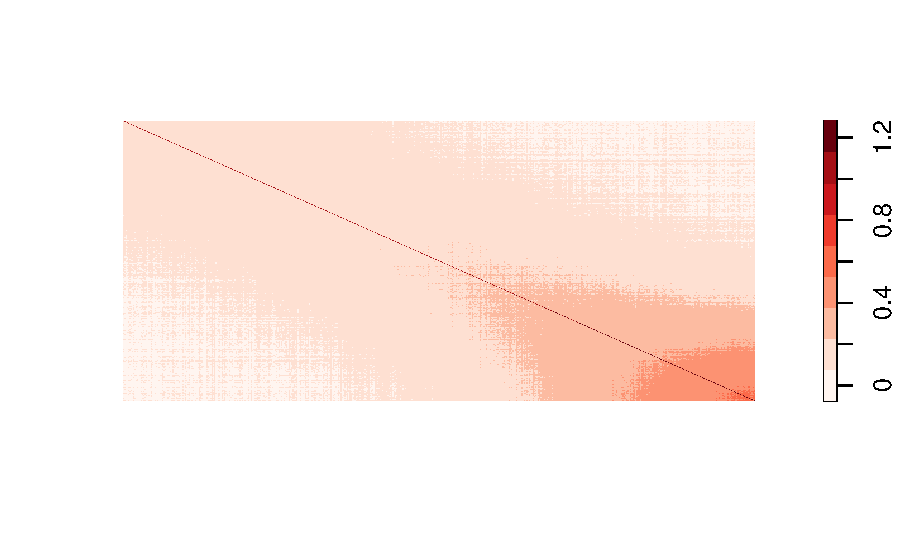
\includegraphics[width=1\linewidth]{figure/unnamed-chunk-2-1} 

}



\end{knitrout}

\subsection{Fit the linear mixed model with Lasso Penalty}

We will use the most basic call to the main function of this package, which is called \texttt{ggmix}. This function will by default fit a $L_1$ penalized linear mixed model (LMM) for 100 distinct values of the tuning parameter $\lambda$. It will choose its own sequence:  

\begin{knitrout}\scriptsize
\definecolor{shadecolor}{rgb}{0.969, 0.969, 0.969}\color{fgcolor}\begin{kframe}
\begin{alltt}
\hlstd{fit} \hlkwb{<-} \hlkwd{ggmix}\hlstd{(}\hlkwc{x} \hlstd{= admixed}\hlopt{$}\hlstd{x,} \hlkwc{y} \hlstd{= admixed}\hlopt{$}\hlstd{y,} \hlkwc{kinship} \hlstd{= admixed}\hlopt{$}\hlstd{kin)}
\hlkwd{names}\hlstd{(fit)}
\end{alltt}
\begin{verbatim}
##  [1] "result"       "ggmix_object" "n_design"     "p_design"    
##  [5] "lambda"       "coef"         "b0"           "beta"        
##  [9] "df"           "eta"          "sigma2"       "nlambda"     
## [13] "cov_names"    "call"
\end{verbatim}
\begin{alltt}
\hlkwd{class}\hlstd{(fit)}
\end{alltt}
\begin{verbatim}
## [1] "lassofullrank" "ggmix_fit"
\end{verbatim}
\end{kframe}
\end{knitrout}

We can see the solution path for each variable by calling the \texttt{plot} method for objects of class \texttt{ggmix\_fit}:  

\begin{knitrout}\scriptsize
\definecolor{shadecolor}{rgb}{0.969, 0.969, 0.969}\color{fgcolor}\begin{kframe}
\begin{alltt}
\hlkwd{plot}\hlstd{(fit)}
\end{alltt}
\end{kframe}

{\centering 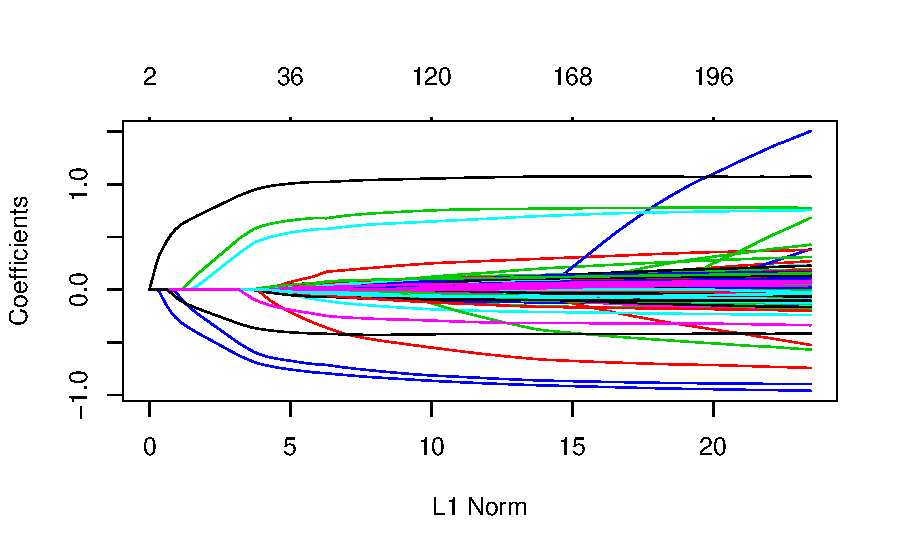
\includegraphics[width=1\linewidth]{figure/unnamed-chunk-4-1} 

}



\end{knitrout}

We can also get the coefficients for given value(s) of lambda using the \texttt{coef} method for objects of class \texttt{ggmix\_fit}:  

\begin{knitrout}\scriptsize
\definecolor{shadecolor}{rgb}{0.969, 0.969, 0.969}\color{fgcolor}\begin{kframe}
\begin{alltt}
\hlcom{# only the first 5 coefficients printed here for brevity}
\hlkwd{coef}\hlstd{(fit,} \hlkwc{s} \hlstd{=} \hlkwd{c}\hlstd{(}\hlnum{0.1}\hlstd{,}\hlnum{0.02}\hlstd{))[}\hlnum{1}\hlopt{:}\hlnum{5}\hlstd{, ]}
\end{alltt}
\begin{verbatim}
## 5 x 2 Matrix of class "dgeMatrix"
##                      1            2
## (Intercept) -0.3824525 -0.030227753
## X62          0.0000000  0.000000000
## X185         0.0000000  0.001444670
## X371         0.0000000  0.009513604
## X420         0.0000000  0.000000000
\end{verbatim}
\end{kframe}
\end{knitrout}
Here, \texttt{s} specifies the value(s) of $\lambda$ at which the extraction is made. The function uses linear interpolation to make predictions for values of \texttt{s} that do not coincide with the lambda sequence used in the fitting algorithm.  

We can also get predictions ($X\widehat{\boldsymbol{\beta}}$) using the \texttt{predict} method for objects of class \texttt{ggmix\_fit}:  

\begin{knitrout}\scriptsize
\definecolor{shadecolor}{rgb}{0.969, 0.969, 0.969}\color{fgcolor}\begin{kframe}
\begin{alltt}
\hlcom{# need to provide x to the predict function}
\hlcom{# predict for the first 5 subjects }
\hlkwd{predict}\hlstd{(fit,} \hlkwc{s} \hlstd{=} \hlkwd{c}\hlstd{(}\hlnum{0.1}\hlstd{,}\hlnum{0.02}\hlstd{),} \hlkwc{newx} \hlstd{= admixed}\hlopt{$}\hlstd{x[}\hlnum{1}\hlopt{:}\hlnum{5}\hlstd{,])}
\end{alltt}
\begin{verbatim}
##               1          2
## id1 -1.19165061 -1.3123396
## id2 -0.02913052  0.3885921
## id3 -2.00084875 -2.6460045
## id4 -0.37255277 -0.9542455
## id5 -1.03967831 -2.1377274
\end{verbatim}
\end{kframe}
\end{knitrout}


\subsection{Find the Optimal Value of the Tuning Parameter}

We use the Generalized Information Criterion (GIC) to select the optimal value for $\lambda$. The default is $a_n = log(log(n)) * log(p)$ which corresponds to a high-dimensional BIC (HDBIC): 

\begin{knitrout}\scriptsize
\definecolor{shadecolor}{rgb}{0.969, 0.969, 0.969}\color{fgcolor}\begin{kframe}
\begin{alltt}
\hlcom{# pass the fitted object from ggmix to the gic function:}
\hlstd{hdbic} \hlkwb{<-} \hlkwd{gic}\hlstd{(fit)}
\hlkwd{class}\hlstd{(hdbic)}
\end{alltt}
\begin{verbatim}
## [1] "ggmix_gic"     "lassofullrank" "ggmix_fit"
\end{verbatim}
\begin{alltt}
\hlcom{# we can also fit the BIC by specifying the an argument}
\hlstd{bicfit} \hlkwb{<-} \hlkwd{gic}\hlstd{(fit,} \hlkwc{an} \hlstd{=} \hlkwd{log}\hlstd{(}\hlkwd{length}\hlstd{(admixed}\hlopt{$}\hlstd{y)))}
\end{alltt}
\end{kframe}
\end{knitrout}

We can plot the HDBIC values against $\log(\lambda)$ using the \texttt{plot} method for objects of class \texttt{ggmix\_gic}:  

\begin{knitrout}\scriptsize
\definecolor{shadecolor}{rgb}{0.969, 0.969, 0.969}\color{fgcolor}\begin{kframe}
\begin{alltt}
\hlkwd{plot}\hlstd{(hdbic)}
\end{alltt}
\end{kframe}

{\centering 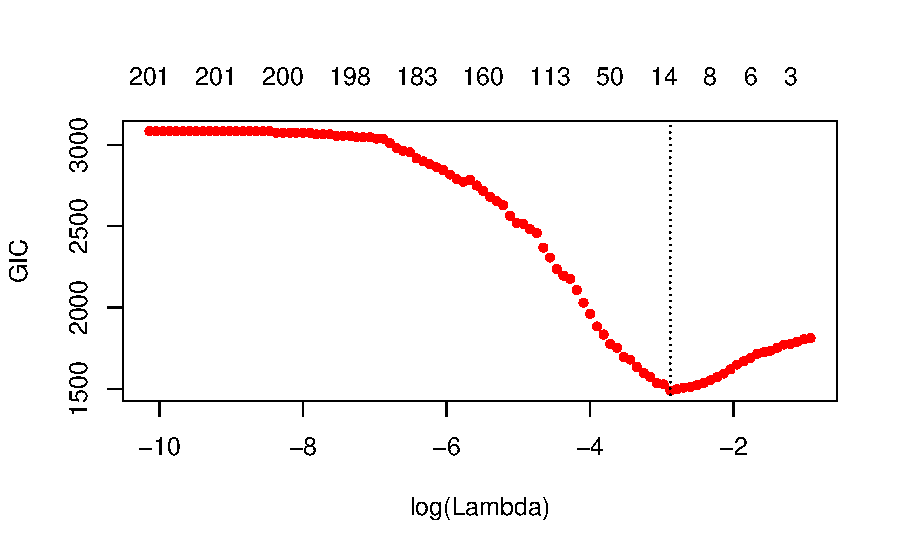
\includegraphics[width=1\linewidth]{figure/unnamed-chunk-8-1} 

}



\end{knitrout}

The optimal value for $\lambda$ according to the HDBIC, i.e., the $\lambda$ that leads to the minium HDBIC is:

\begin{knitrout}\scriptsize
\definecolor{shadecolor}{rgb}{0.969, 0.969, 0.969}\color{fgcolor}\begin{kframe}
\begin{alltt}
\hlstd{hdbic[[}\hlstr{"lambda.min"}\hlstd{]]}
\end{alltt}
\begin{verbatim}
## [1] 0.05596623
\end{verbatim}
\end{kframe}
\end{knitrout}


We can also plot the BIC results:

\begin{knitrout}\scriptsize
\definecolor{shadecolor}{rgb}{0.969, 0.969, 0.969}\color{fgcolor}\begin{kframe}
\begin{alltt}
\hlkwd{plot}\hlstd{(bicfit,} \hlkwc{ylab} \hlstd{=} \hlstr{"BIC"}\hlstd{)}
\end{alltt}
\end{kframe}

{\centering 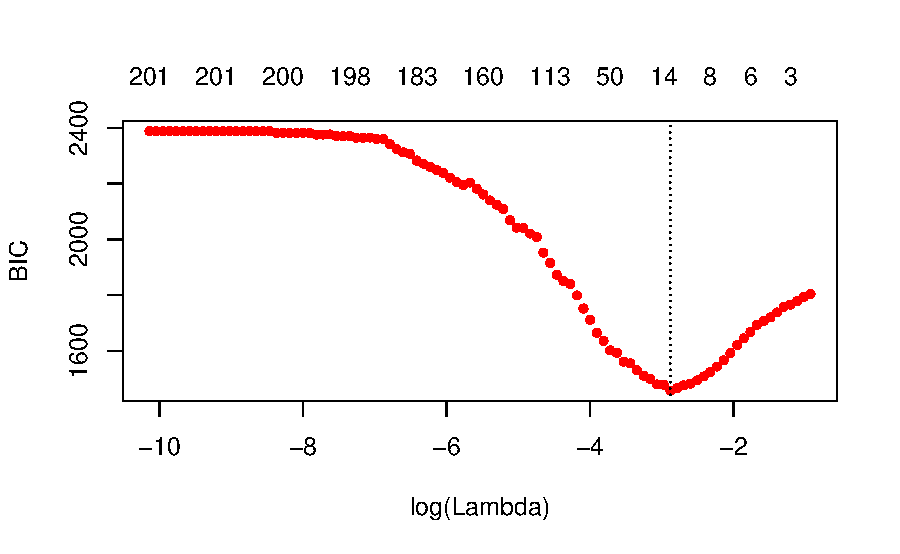
\includegraphics[width=1\linewidth]{figure/unnamed-chunk-10-1} 

}


\begin{kframe}\begin{alltt}
\hlstd{bicfit[[}\hlstr{"lambda.min"}\hlstd{]]}
\end{alltt}
\begin{verbatim}
## [1] 0.05596623
\end{verbatim}
\end{kframe}
\end{knitrout}


\subsection{Get Coefficients Corresponding to Optimal Model}

We can use the object outputted by the \texttt{gic} function to extract the coefficients corresponding to the selected model using the \texttt{coef} method for objects of class \texttt{ggmix\_gic}:  

\begin{knitrout}\scriptsize
\definecolor{shadecolor}{rgb}{0.969, 0.969, 0.969}\color{fgcolor}\begin{kframe}
\begin{alltt}
\hlkwd{coef}\hlstd{(hdbic)[}\hlnum{1}\hlopt{:}\hlnum{5}\hlstd{, ,} \hlkwc{drop} \hlstd{=} \hlnum{FALSE}\hlstd{]}
\end{alltt}
\begin{verbatim}
## 5 x 1 sparse Matrix of class "dgCMatrix"
##                      1
## (Intercept) -0.2668419
## X62          .        
## X185         .        
## X371         .        
## X420         .
\end{verbatim}
\end{kframe}
\end{knitrout}

We can also extract just the nonzero coefficients which also provide the estimated variance components $\eta$ and $\sigma^2$:

\begin{knitrout}\scriptsize
\definecolor{shadecolor}{rgb}{0.969, 0.969, 0.969}\color{fgcolor}\begin{kframe}
\begin{alltt}
\hlkwd{coef}\hlstd{(hdbic,} \hlkwc{type} \hlstd{=} \hlstr{"nonzero"}\hlstd{)}
\end{alltt}
\begin{verbatim}
##                       1
## (Intercept) -0.26684191
## X336        -0.67986393
## X7638        0.43403365
## X1536        0.93994982
## X1943        0.56600730
## X2849       -0.58157979
## X56         -0.08244685
## X4106       -0.35939830
## eta          0.26746240
## sigma2       0.98694300
\end{verbatim}
\end{kframe}
\end{knitrout}

We can also make predictions from the \texttt{hdbic} object, which by default will use the model corresponding to the optimal tuning parameter:

\begin{knitrout}\scriptsize
\definecolor{shadecolor}{rgb}{0.969, 0.969, 0.969}\color{fgcolor}\begin{kframe}
\begin{alltt}
\hlkwd{predict}\hlstd{(hdbic,} \hlkwc{newx} \hlstd{= admixed}\hlopt{$}\hlstd{x[}\hlnum{1}\hlopt{:}\hlnum{5}\hlstd{,])}
\end{alltt}
\begin{verbatim}
##              1
## id1 -1.3061041
## id2  0.2991654
## id3 -2.3453664
## id4 -0.4486012
## id5 -1.3895793
\end{verbatim}
\end{kframe}
\end{knitrout}


\subsection{Extracting Random Effects}

The user can compute the random effects using the provided \texttt{ranef} method for objects of class \texttt{ggmix\_gic}. This command will compute the estimated random effects for each subject using the parameters of the selected model:

\begin{knitrout}\scriptsize
\definecolor{shadecolor}{rgb}{0.969, 0.969, 0.969}\color{fgcolor}\begin{kframe}
\begin{alltt}
\hlkwd{ranef}\hlstd{(hdbic)[}\hlnum{1}\hlopt{:}\hlnum{5}\hlstd{]}
\end{alltt}
\begin{verbatim}
## [1] -0.02548691 -0.10011680  0.13020240 -0.30650997  0.16045768
\end{verbatim}
\end{kframe}
\end{knitrout}



\subsection{Diagnostic Plots}

We can also plot some standard diagnotic plots such as the observed vs. predicted response, QQ-plots of the residuals and random effects and the Tukey-Anscombe plot. These can be plotted using the \texttt{plot} method on a \texttt{ggmix\_gic} object as shown below.


\subsubsection{Observed vs. Predicted Response}

\begin{knitrout}\scriptsize
\definecolor{shadecolor}{rgb}{0.969, 0.969, 0.969}\color{fgcolor}\begin{kframe}
\begin{alltt}
\hlkwd{plot}\hlstd{(hdbic,} \hlkwc{type} \hlstd{=} \hlstr{"predicted"}\hlstd{,} \hlkwc{newx} \hlstd{= admixed}\hlopt{$}\hlstd{x,} \hlkwc{newy} \hlstd{= admixed}\hlopt{$}\hlstd{y)}
\end{alltt}
\end{kframe}

{\centering 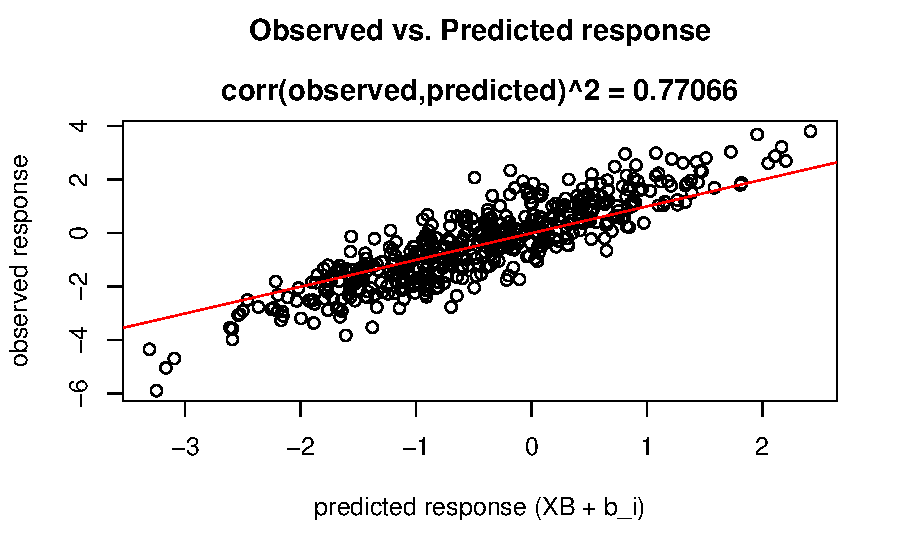
\includegraphics[width=1\linewidth]{figure/unnamed-chunk-15-1} 

}



\end{knitrout}


\subsubsection{QQ-plots for Residuals and Random Effects}

\begin{knitrout}\scriptsize
\definecolor{shadecolor}{rgb}{0.969, 0.969, 0.969}\color{fgcolor}\begin{kframe}
\begin{alltt}
\hlkwd{plot}\hlstd{(hdbic,} \hlkwc{type} \hlstd{=} \hlstr{"QQranef"}\hlstd{,} \hlkwc{newx} \hlstd{= admixed}\hlopt{$}\hlstd{x,} \hlkwc{newy} \hlstd{= admixed}\hlopt{$}\hlstd{y)}
\end{alltt}
\end{kframe}

{\centering 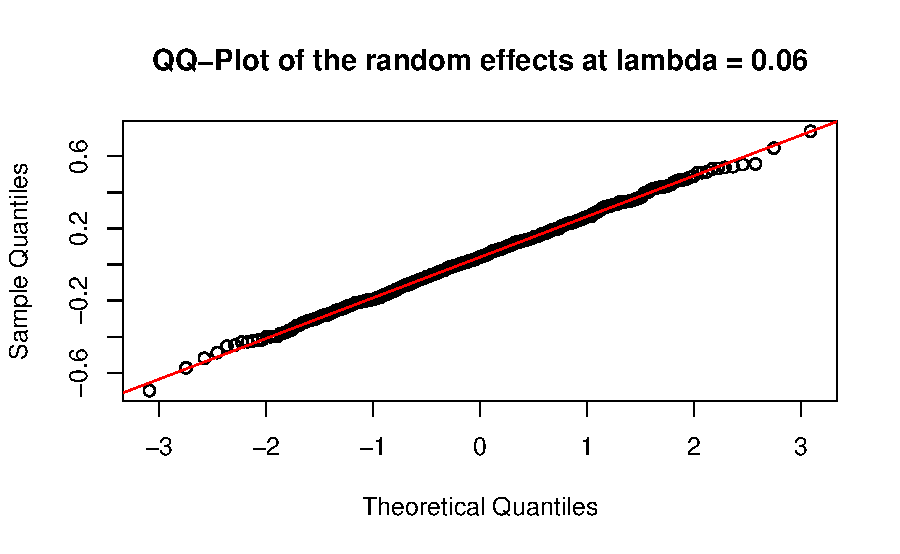
\includegraphics[width=1\linewidth]{figure/unnamed-chunk-16-1} 

}


\begin{kframe}\begin{alltt}
\hlkwd{plot}\hlstd{(hdbic,} \hlkwc{type} \hlstd{=} \hlstr{"QQresid"}\hlstd{,} \hlkwc{newx} \hlstd{= admixed}\hlopt{$}\hlstd{x,} \hlkwc{newy} \hlstd{= admixed}\hlopt{$}\hlstd{y)}
\end{alltt}
\end{kframe}

{\centering 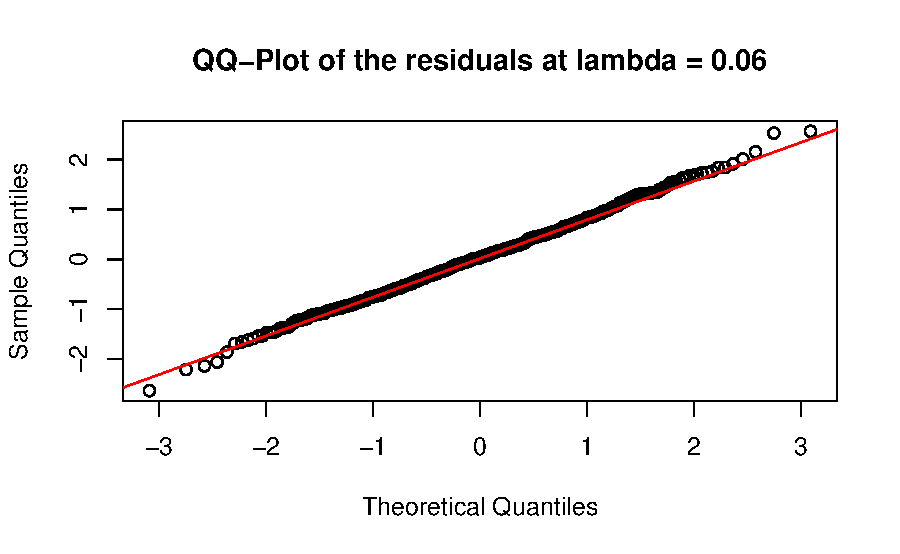
\includegraphics[width=1\linewidth]{figure/unnamed-chunk-16-2} 

}



\end{knitrout}


\subsubsection{Tukey-Anscombe Plot}

\begin{knitrout}\scriptsize
\definecolor{shadecolor}{rgb}{0.969, 0.969, 0.969}\color{fgcolor}\begin{kframe}
\begin{alltt}
\hlkwd{plot}\hlstd{(hdbic,} \hlkwc{type} \hlstd{=} \hlstr{"Tukey"}\hlstd{,} \hlkwc{newx} \hlstd{= admixed}\hlopt{$}\hlstd{x,} \hlkwc{newy} \hlstd{= admixed}\hlopt{$}\hlstd{y)}
\end{alltt}
\end{kframe}

{\centering 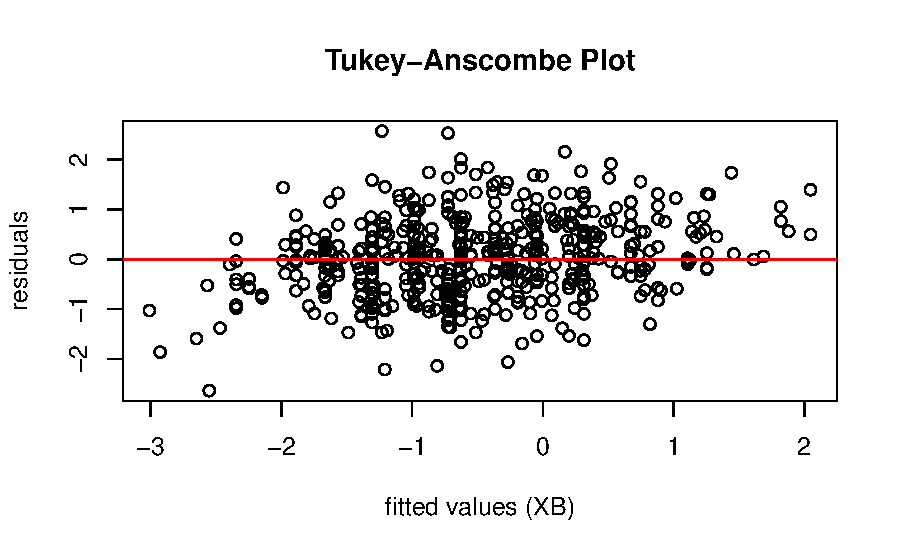
\includegraphics[width=1\linewidth]{figure/unnamed-chunk-17-1} 

}



\end{knitrout}






\end{document}

\section{Low rank similarity matrix}

Let $\mb{K} \in \mathbb{R}^{N_T\times k}$ be the matrix containing the $k$ SNPs used to compute the factored kinship matrix $\bPhi$ given by
\begin{equation}
	\bPhi = \mb{K}\mb{K}^T \label{eq:factored}
\end{equation}

%If we let $\mb{U} \mb{\widetilde{S}} \mb{V}^T$ be the singular value decomposition (SVD) of $\mb{K}$. Then
%\begin{align*}
%\bPhi &= \left(\mb{U} \mb{\widetilde{S}} \mb{V}^T\right)\left(\mb{U} \mb{\widetilde{S}} \mb{V}^T\right)^T \\
%& = \mb{U}\mb{\widetilde{S}}\mb{V}^T\mb{V}\mb{\widetilde{S}}\mb{U}^T\\
%& = \mb{U} \mb{\widetilde{S}}\mb{\widetilde{S}}\mb{U}^T \\
%& = \mb{U} \mb{S} \mb{U}^T
%\end{align*}
%where $\mb{S}_{ii} = \mb{\widetilde{S}}_{ii}\mb{\widetilde{S}}_{ii}$. Therefore, $\mb{U}$ consists of the eigenvectors of $\bPhi$ and the eigenvalues of $\bPhi$ are given by %$\mb{\widetilde{S}}_{ii}^2$ which are the square of the eigenvalues of the SNP matrix $\mb{K} \in \mathbb{R}^{n\times p}$.
%Note that the eigenvectors of $\bPhi$ are equal to the singular vectors of $\mb{K}$, and the eigenvalues of $\bPhi$ are equal to the square of the singular values of %$\mb{K}$~\citep{berrar2003practical}.

Furthermore, let $\mb{K} = \mb{U} \bLambda \mb{V}^T$ be the singular value decomposition (SVD) of $\mb{K}$. Plugging this into~\eqref{eq:factored} we get
\begin{align}
	\bPhi &= \left(\mb{U} \bLambda \mb{V}^T\right)\left(\mb{U} \bLambda \mb{V}^T\right)^T \nonumber\\
	& = \mb{U}\bLambda\mb{V}^T\mb{V}\bLambda\mb{U}^T \nonumber\\
	& = \mb{U} \bLambda\bLambda\mb{U}^T \nonumber\\
	& = \mb{U} \bSigma \mb{U}^T, \label{eq:svdphi}
\end{align}
Therefore, the eigenvectors of $\bPhi$ are equal to the singular vectors of $\mb{K}$ (denoted by $\bU$), and the eigenvalues of $\bPhi$ (denoted by the diagonal matrix $\bSigma$) are equal to the square of the singular values of $\mb{K}$~\citep{berrar2003practical}. This allows us to bypass the explicit computation of the kinship matrix by directly applying SVD on the SNP matrix $\bW$. ~\cite{lippert2011fast} noted that the computational time for fitting the LMM can be reduced if the matrix $\mb{K}$ is not full rank, i.e., when $k < N_T$. This is due to the fact that the matrix $\bD_{N_T \times N_T}$ contains $k$ non-zero eigenvalues followed by $N_T-k$ zeros on the diagonal. Let $\bU \equiv \left[\bU_1 \,\, \bU_2\right]$, where $\bU_1 \in \mathbb{R}^{N_T\times k}$ and $\bU_2 \in \mathbb{R}^{N_T \times (n-k)}$ are  the matrices of singular vectors corresponding to the $k$ non-zero and $N_T-k$ zero eigenvalues, respectively. Then~\eqref{eq:svdphi} can be written as
\begin{equation}
	\bPhi = \bU_1 \bSigma \bU_1^T
\end{equation}
%Following~\cite{lippert2011fast}, we show that the log-likelihood~\eqref{eq:Likelihood} can be expressed in terms of $\bU_1$ only, foregoing the need to compute $\bU_2$.
We now try to simplify the log-likelihood~\eqref{eq:Likelihood}. Since there are $N_T-k$ zero eigenvalues, the second term in~\eqref{eq:Likelihood} reduces to
\begin{equation}
	\frac{1}{2} \left(  \sum_{i=1}^{k} \log(1 + \eta (\Sigma_i-1)) + (N_T-k) \log(1-\eta)\right) \label{eq:term2}
\end{equation}
where $\Sigma_i = \Lambda_i^2$, and $\Lambda_i$ is the $i^{\tm{th}}$ singular value of $\bW$. Let $a \equiv (\bY - \bX \bbeta)$. The third term in~\eqref{eq:Likelihood} can be written as
\begin{align}
	\frac{1}{2\sigma^2} a^T \left[ \eta \bPhi + (1-\eta)\bI_n \right] ^{-1} a &= \frac{1}{2\sigma^2} a^T \left[ \eta \bU_1 \bSigma_1 \bU_1^T + (1-\eta)\bI_n \right] ^{-1} a  \nonumber \\
	& = \frac{1}{2\sigma^2} a^T \left[ \bC \bB \bC^T + \mb{A} \right] ^{-1} a \nonumber
\end{align}
where
\begin{align*}
	\mb{A} & = (1-\eta) \bI_n \\
	\mb{B} & = \bSigma_1 \\
	\mb{C} & = \sqrt{\eta} \bU_1 \\
	\mb{C}^T & = \sqrt{\eta} \bU_1^T
\end{align*}
Assuming $\bC \bB \bC^T + \mb{A}$ is non-singular, the inverse of $\left[ \bC \bB \bC^T + \mb{A} \right]$ is given explicitly by the Woodbury formula~\citep{golub2012matrix}
\begin{align}
	\left(\bA + \bC \bB \bC^T\right)^{-1} & = \bA^{-1} - \bA^{-1} \bC \left(\bB^{-1} + \bC^T\bA^{-1} \bC\right)^{-1}\bC^T \bA^{-1} \label{eq:woodbury}
\end{align}
Substituting the values for $\bA, \bB$ and $\bC$ into~\eqref{eq:woodbury} we get
\begin{align}
	\left(\bA + \bC \bB \bC^T\right)^{-1} & = \frac{1}{1-\eta}\bI_{N_T} - \frac{\sqrt{\eta}}{1-\eta}\bI_{N_T}\bU_1 \left(\bSigma_1^{-1} + \frac{\eta}{1-\eta}\bU_1^T \bI_{N_T} \bU\right)^{-1}\frac{\sqrt{\eta}}{1-\eta}\bU_1^T \bI_{N_T} \nonumber \\
	& = \frac{1}{1-\eta} \left[ \bI_{N_T} - \frac{\eta}{1-\eta}\bU_1 \left(\bSigma_1^{-1} + \frac{\eta}{1-\eta}\bI_{k} \right)^{-1}\bU_1^T \right] \nonumber \\
	& = \frac{1}{1-\eta} \left[ \bI_{N_T} - \frac{\eta}{1-\eta}\bU_1 \left(\frac{\eta}{1-\eta} \left(\frac{1-\eta}{\eta}\bSigma_1^{-1} + \bI_{k}\right) \right)^{-1}\bU_1^T \right] \nonumber \\
	& = \frac{1}{1-\eta} \left[ \bI_{N_T} - \bU_1 \left(\frac{1-\eta}{\eta}\bSigma_1^{-1} + \bI_{k}\right) ^{-1}\bU_1^T \right] \label{eq:term3}
\end{align}


where we have used the following identities: $\bI_k = \bU_1^T\bU_1$, $\bI_{N_T -k} = \bU_2^T\bU_2$.
%, and
%\begin{align}
%\bI_{N_T} & = \bU \bU^T  \nonumber\\
%& =\left[\bU_1 \,\, \bU_2\right] \left[\bU_1 \,\, \bU_2\right] ^T \nonumber\\
%& = \bU_1 \bU_1^T + \bU_2 \bU_2^T \label{eq:In} \nonumber
%\end{align}

Substituting~\eqref{eq:term2} and~\eqref{eq:term3} in~\eqref{eq:Likelihood} we obtain
\begin{align}
	\begin{split}
		-\ell(\bTheta) & \propto \frac{N_T}{2}\log(\sigma^2) + \frac{1}{2} \left(  \sum_{i=1}^{k} \log(1 + \eta (\Sigma_i-1)) + (N_T-k) \log(1-\eta)\right) + \\
		&\frac{1}{2} \left\lbrace \left(\bY - \bX\bbeta \right)^T  \left[\frac{1}{\sigma^2(1-\eta)}\left(  \bI_{N_T} - \bU_1 \left(\frac{1-\eta}{\eta}\bSigma_1^{-1} + \bI_{k}\right) ^{-1}\bU_1^T \right)  \right] \left(\bY - \bX\bbeta \right)  \right\rbrace
	\end{split} \label{eq:loglikrowrank}
\end{align}

\section{Group Lasso with Low-rank Similarity Matrix}
This section focuses on the part of the log-likelihood~\eqref{eq:loglikrowrank} that depends on $\bbeta$.

\subsection{Model}
Only the third term of the log-likelihood~\eqref{eq:loglikrowrank} depends on $\bbeta$:
\begin{equation}
	\frac{1}{2} \left\lbrace \left(\bY - \bX\bbeta \right)^T  \left[\frac{1}{\sigma^2(1-\eta)}\left(  \bI_{N_T} - \bU_1 \left(\frac{1-\eta}{\eta}\bSigma_1^{-1} + \bI_{k}\right) ^{-1}\bU_1^T \right)  \right] \left(\bY - \bX\bbeta \right)  \right\rbrace \label{eq:likeW}
\end{equation}
Equation~\eqref{eq:likeW} can be written more generally as
\[
L(\bbeta\mid\bD)=\frac{1}{2}\left[\bY-\widehat{\bY}\right]^{\top}\mathbf{W}\left[\bY-\widehat{\bY}\right]
\]
where $\widehat{\bY}=\sum_{j=1}^{p}\beta_{j}X_{j}$, $\bD$ is the working data $\lbrace \bY, \bX \rbrace$, and $\bW$ is an $N_T \times N_T$ weight matrix given by
\begin{equation}
	\bW = \frac{1}{\sigma^2(1-\eta)}\left(  \bI_{N_T} - \bU_1 \left(\frac{1-\eta}{\eta}\bSigma_1^{-1} + \bI_{k}\right) ^{-1}\bU_1^T \right)   \label{eq:weight}
\end{equation}

%Consider the linear regression problem where we have a continuous response $\by\in\mathbb{R}^{n}$
%and let $\bX$ be the design matrix with $n$ rows and $p$ columns where $n$ is the sample size of the raw data. If an intercept is used in the model, we let the first column of $\bX$ be a vector of 1.
Assume that we the predictors in the design matrix $\bX \in \mathbb{R}^{N_T \times p}$ belong to $K$ groups and that the group membership is already defined such that $(1,2,\ldots,p)=\bigcup_{k=1}^{K}I_{k}$ and the cardinality of index set $I_{k}$ is $p_{k}$, $I_{k}\bigcap I_{k^{\prime}}=\emptyset$ for $k\neq k^{\prime},1\le k,k^{\prime}\le K$. Thus group $k$ contains $p_{k}$ predictors, which are $x_{j}$'s for $j\in I_{k}$, and $1\le k\le K.$ If an intercept is included, then $I_{1}=\{1\}$. Given the group partition, we use $\bbeta_{(k)}$ to denote the segment of $\bbeta$ corresponding to group $k$. This notation is used for any $p$-dimensional vector.
%In a more compact form, and introducing observation weights
%\[
%L(\bbeta\mid\bD)=\frac{1}{2}\left[Y-\hat{Y}\right]^{\top}\mathbf{W}\left[Y-\hat{Y}\right]
%\]
%where $\hat{Y}=\sum_{j=1}^{p}\beta_{j}X_{j}$, $\bD$ is the working data $\lbrace \by, \bX \rbrace$, $\bW$ is an $N_T \times N_T$ weight matrix. Then the problem we consider can be expressed as
We consider the group lasso penalized estimator
\begin{equation}
	\min_{\bbeta}L(\bbeta \mid \bD)+\lambda\sum_{k=1}^{K}w_{k}\|\bbk\|_{2},\label{eq:wlslasso}
\end{equation}

The loss function $L$ satisfies the quadratic majorization (QM) condition, since there exists
a $p\times p$ matrix $\bH=\bX^{\trans}\mathbf{W}\bX$, and $\nabla L(\bbeta|\bD)=-\left(Y-\hat{Y}\right)^{\top}\mathbf{W}\bX$, which may only depend on the data $\bD$, such that for all $\bbeta,\bbeta^{*}$,
\begin{equation}
	L(\bbeta\mid\bD)\le L(\bbeta^{*}\mid\bD)+(\bbeta-\bbeta^{*})^{\trans}\nabla L(\bbeta^{*}|\bD)+\frac{1}{2}(\bbeta-\bbeta^{*})^{\trans}\bH(\bbeta-\bbeta^{*}).\label{QM1}
\end{equation}

\subsection{Algorithm}

Noticing that the penalty term $\sum_{k=1}^{K}w_{k}||\bbeta_{(k)}||_{2}$ is separable with respect to the indices of the features $k=1, \ldots, K$, we can derive the \textit{groupwise-majorization-descent} (GMD) algorithm for computing the solution of~\eqref{eq:wlslasso} when the loss function satisfies the QM condition. Let $\widetilde{\bbeta}$ denote the current solution of $\bbeta$. Without loss of generality, let us derive the GMD update of $\bbkt$, the coefficients of group $k$. Define $\bH_{k}$ as the sub-matrix of $\bH$ corresponding to group $k$. For example, if group 2 is $\{2,4\}$ then $\bH_{(2)}$ is a $2\times2$ matrix with
\[
\bH_{(2)}=\left[\begin{array}{cc}
h_{2,2} & h_{2,4}\\
h_{4,2} & h_{4,4}
\end{array}\right],
\]

where $h_{i,j}$ is the $i,j$th entry of the $\bH$ matrix. Write $\bbeta$ such that $\bbeta_{(k^{\prime})}=\widetilde{\bbeta}_{(k^{\prime})}$ for $k^{\prime}\ne k$. Given $\bbeta_{(k^{\prime})}=\widetilde{\bbeta}_{(k^{\prime})}$ for $k^{\prime}\ne k$, the optimal $\bbk$ is defined as
\begin{equation}
	\arg\min_{\boldsymbol{\beta}^{(k)}}L(\bbeta\mid\bD)+\lambda w_{k}\Vert\bbk\Vert_{2}.\label{GMDeq1}
\end{equation}
Unfortunately, there is no closed form solution to~\eqref{GMDeq1} for a general loss function with general design matrix. We overcome the computational obstacle by taking advantage of the QM condition. From~\eqref{QM1} we have
\[
L(\bbeta\mid\bD)\le L(\widetilde{\bbeta}\mid\bD)+(\bbeta-\widetilde{\bbeta})^{\trans}\nabla L(\widetilde{\bbeta}|\bD)+\frac{1}{2}(\bbeta-\widetilde{\bbeta})^{\trans}\bH(\bbeta-\widetilde{\bbeta}).
\]

Write $U(\widetilde{\bbeta})=-\nabla L(\widetilde{\bbeta}|\bD)$. Using
\[
\bbeta-\widetilde{\bbeta}=(\underbrace{0,\ldots,0}_{k-1},\bbk-\bbkt,\underbrace{0,\ldots,0}_{K-k}),
\]
we can write
\begin{equation}
	L(\bbeta\mid\bD)\le L(\widetilde{\bbeta}\mid\bD)-(\bbk-\bbkt)^{\trans}U_{(k)}+\frac{1}{2}(\bbk-\bbkt)^{\trans}\bH_{(k)}(\bbk-\bbkt).\label{GMDeq2}
\end{equation}
where
\begin{align}
	U_{(k)} & =\frac{\partial}{\partial\bbk}L_{Q}(\bbeta\mid\bD)=-\left(Y-\hat{Y}\right)^{\top}\mathbf{W}\mathbf{X}_{(k)},\label{eq:gradientj-1}\\
	\mathbf{H}_{(k)} & =\frac{\partial^{2}}{\partial\bbk\partial\bbk^{\top}}L_{Q}(\bbeta\mid\bD)=\mathbf{X}_{(k)}^{\top}\mathbf{W}\mathbf{X}_{(k)}.\label{eq:hessianj-1}
\end{align}

Let $\eta_{k}$ be the largest eigenvalue of $\bH_{(k)}$. We set $\gamma_{k}=(1+\varepsilon^{*})\eta_{k}$, where $\varepsilon^{*}=10^{-6}$. Then we can further relax the upper bound in~\eqref{GMDeq2} as
\begin{equation}
	L(\bbeta\mid\bD)\leq L(\widetilde{\bbeta}\mid\bD)-(\bbeta^{(k)}-\widetilde{\bbeta}^{(k)})^{\trans}U_{(k)}+\frac{1}{2}\gamma_{k}(\bbeta^{(k)}-\widetilde{\bbeta}^{(k)})^{\trans}(\bbeta^{(k)}-\widetilde{\bbeta}^{(k)}).\label{GMDeq3-1}
\end{equation}
It is important to note that the inequality strictly holds unless for $\bbeta^{(k)}=\widetilde{\bbeta}^{(k)}$. Instead of minimizing~\eqref{GMDeq1} we solve
\begin{equation}
	\arg\min_{\bbeta^{(k)}}L(\widetilde{\bbeta}\mid\bD)-(\bbeta^{(k)}-\widetilde{\bbeta}^{(k)})^{\trans}U_{(k)}+\frac{1}{2}\gamma_{k}(\bbeta^{(k)}-\widetilde{\bbeta}^{(k)})^{\trans}(\bbeta^{(k)}-\widetilde{\bbeta}^{(k)})+\lambda w_{k}\Vert\bbeta^{(k)}\Vert_{2}.\label{GMDeq4-1}
\end{equation}

Denote by $\widetilde{\bbeta}^{(k)}(\textrm{new})$ the solution to~\eqref{GMDeq4-1}. It is straightforward to see that $\widetilde{\bbeta}^{(k)}(\textrm{new})$ has a simple closed-from expression
\begin{equation}
	\widetilde{\bbeta}^{(k)}(\textrm{new})=\frac{1}{\gamma_{k}}\left(U^{(k)}+\gamma_{k}\widetilde{\bbeta}^{(k)}\right)\left(1-\frac{\lambda w_{k}}{\Vert U^{(k)}+\gamma_{k}\widetilde{\bbeta}^{(k)}\Vert_{2}}\right)_{+}.\label{GMDeq5-1}
\end{equation}

Algorithm~\ref{alg1} summarizes the details of GMD.

\begin{algorithm}
	\begin{enumerate}
		\item For $k=1,\ldots,K$, compute $\gamma_k$, the largest eigenvalue of $\bH^{(k)}$.
		\item Initialize $\widetilde \bbeta$.
		\item Repeat the following cyclic groupwise updates until convergence:
		\begin{enumerate}
			\item[---] for $k=1,\ldots,K$, do step (3.1)--(3.3)
			\begin{enumerate}
				\item[3.1]
				Compute $U(\widetilde \bbeta )=-\nabla L(\widetilde \bbeta | \bD)$.
				\item[3.2]
				Compute
				$
				\widetilde \bbeta^{(k)}(\textrm{new}) = \frac{1}{\gamma_k}\left( U^{(k)}+\gamma_k \widetilde \bbeta^{(k)} \right)\left(1-\frac{\lambda w_k}{\Vert U^{(k)}+\gamma_k \widetilde \bbeta^{(k)} \Vert_2}\right)_{+} .
				$
				\item[3.3]
				Set $\widetilde \bbeta^{(k)}=\widetilde \bbeta^{(k)}(\textrm{new})$.
			\end{enumerate}
		\end{enumerate}
	\end{enumerate}
	\caption{The GMD algorithm for general group-lasso learning. \label{alg1}}
\end{algorithm}


\subsection{Convergence}

We can prove the strict descent property of GMD by using the MM principle \citep{MM1,hunter2004tutorial,MM08}. Define
\begin{equation}
	Q(\bbeta \mid \bD)=L(\widetilde \bbeta \mid \bD)-(\bbeta^{(k)}-\widetilde \bbeta^{(k)})^{\trans}
	U^{(k)}+\frac{1}{2} \gamma_k (\bbeta^{(k)}-\widetilde \bbeta^{(k)})^{\trans} ( \bbeta^{(k)}- \widetilde \bbeta^{(k)})+\lambda w_k \Vert \bbeta^{(k)}\Vert_2.
\end{equation}
Obviously, $Q(\bbeta \mid \bD)=L(\bbeta \mid \bD)+\lambda w_k \Vert \bbeta^{(k)}\Vert_2$ when $\bbeta^{(k)}=\widetilde \bbeta^{(k)}$ and
(\ref{GMDeq3}) shows that
$Q(\bbeta \mid \bD) > L(\bbeta \mid \bD)+\lambda w_k \Vert \bbeta^{(k)}\Vert_2$ when $\bbeta^{(k)} \neq \widetilde \bbeta^{(k)}$.
After updating $\widetilde \bbeta^{(k)}$ using (\ref{GMDeq5}), we have
\begin{eqnarray*}
	L(\widetilde \bbeta^{(k)}(\textrm{new}) \mid \bD)+\lambda w_k \Vert \widetilde \bbeta^{(k)}(\textrm{new}) \Vert_2
	&  \le &  Q(\widetilde \bbeta^{(k)}(\textrm{new})  \mid \bD)\\
	& \le & Q(\widetilde \bbeta  \mid \bD) \\
	& = & L(\widetilde \bbeta \mid \bD)+\lambda w_k \Vert \widetilde \bbeta^{(k)}\Vert_2.
\end{eqnarray*}
Moreover, if $\widetilde \bbeta^{(k)}(\textrm{new}) \neq \widetilde \bbeta^{(k)}$, then the first inequality becomes
\begin{eqnarray*}
	L(\widetilde \bbeta^{(k)}(\textrm{new}) \mid \bD)+\lambda w_k \Vert \widetilde \bbeta^{(k)}(\textrm{new}) \Vert_2
	&  < &  Q(\widetilde \bbeta^{(k)}(\textrm{new})  \mid \bD).
\end{eqnarray*}
Therefore, the objective function is strictly decreased after updating all groups in a cycle, unless the solution does not change after each groupwise update. If this is the case,
we can show that the solution must satisfy the KKT conditions, which means that the algorithm converges and finds the right answer. To see this,
if $\widetilde \bbeta^{(k)}(\textrm{new}) = \widetilde \bbeta^{(k)}$ for all $k$, then by the update formula \eqref{GMDeq5-1} we have that for all $k$
\begin{align}\label{KKTcond1}
	\widetilde \bbeta^{(k)} = \frac{1}{\gamma_k}\left( U^{(k)}+\gamma_k \widetilde \bbeta^{(k)} \right)\left(1-\frac{\lambda w_k}{\Vert U^{(k)}+\gamma_k \widetilde \bbeta^{(k)} \Vert_2}\right) \qquad\textrm{if }\Vert U^{(k)}+\gamma_k \widetilde \bbeta^{(k)} \Vert_2 > \lambda w_{k},\\\label{KKTcond2}
	\widetilde \bbeta^{(k)} = \boldsymbol{0} \qquad\textrm{if }\Vert U^{(k)}+\gamma_k \widetilde \bbeta^{(k)} \Vert_2 \leq \lambda w_{k}.
\end{align}
By straightforward algebra  we obtain the KKT conditions:
\begin{align*}
	-U^{(k)}+\lambda w_{k}\cdot\frac {\widetilde\bbeta^{(k)} }{\Vert\widetilde\bbeta^{(k)}\Vert_2}=\boldsymbol{0}\qquad\textrm{if }\widetilde\bbeta^{(k)}\neq \boldsymbol{0},\\
	\left\Vert
	U^{(k)}
	\right\Vert_2 \le\lambda w_{k}\qquad\textrm{if }\widetilde\bbeta^{(k)}=\boldsymbol{0},
\end{align*}
where $k=1,2,\ldots,K$. Therefore, if the objective function stays unchanged after a cycle, the algorithm necessarily converges to the right
answer.




\subsection{Fitting Options and Algorithms}
Recall $\mb{K} \in \mathbb{R}^{N_T\times k}$ is the matrix containing the $k$ SNPs used to compute the factored kinship matrix $\bPhi$. The dimension of this matrix will determine the algorithm used as shown in the table below.
\ctable[caption={Algorithm used based on dimension of $\mb{K}$. },label=tab:review,pos=h!,doinside=\footnotesize]{LLLLL}{
}{
\FL
Dimension of $\mb{K}$    & lasso   & group lasso \ML
$N_T > k$  			& gcdnet (or degenerate gglasso)  & gglasso (GMD Algorithm with weight matrix) \\
$N_T < k$              & glmnet (Coordinate descent with observation weights)   & gglasso (GMD Algorithm with observation weights)
\LL
}
